\documentclass[review]{elsarticle}
\usepackage{lineno,hyperref}
% package added by zhixuan, not sure whether allowed by JCP or not!
\usepackage{amsmath}
\usepackage{float}

\modulolinenumbers[5]
\journal{Journal of Computational Physics}
%%%%%%%%%%%%%%%%%%%%%%%
%% Elsevier bibliography styles
%%%%%%%%%%%%%%%%%%%%%%%
%% To change the style, put a % in front of the second line of the current style and
%% remove the % from the second line of the style you would like to use.
%%%%%%%%%%%%%%%%%%%%%%%
%% Numbered
\bibliographystyle{model1-num-names}
%% Numbered without titles
%\bibliographystyle{model1a-num-names}
%% Harvard
%\bibliographystyle{model2-names.bst}\biboptions{authoryear}
%% Vancouver numbered
%\usepackage{numcompress}\bibliographystyle{model3-num-names}
%% Vancouver name/year
%\usepackage{numcompress}\bibliographystyle{model4-names}\biboptions{authoryear}
%% APA style
%\bibliographystyle{model5-names}\biboptions{authoryear}
%% AMA style
%\usepackage{numcompress}\bibliographystyle{model6-num-names}
%% `Elsevier LaTeX' style
%\bibliographystyle{elsarticle-num}
%%%%%%%%%%%%%%%%%%%%%%%
\begin{document}
\begin{frontmatter}
\title{A Random Choice SPH Scheme with Adaptive Viscosity}
%\tnotetext[mytitlenote]{Can add  title note here}
%% Group authors per affiliation:
\author{Zhixuan Cao}
\author{Abani Patra \fnref{mycorrespondingauthor}}
\address{Department of Mechanical and Aerospace Engineering, The State University of New York at Buffalo, Amherst, NY, 14260-4200, USA}
\author{E. Bruce Pitman}
\address{Department of Materials Design and Innovation, The State University of New York at Buffalo, Amherst, NY, 14260-4200, USA}
%\fntext[myfootnote]{Since 1880.}
%% or include affiliations in footnotes:
%\author[mymainaddress,mysecondaryaddress]%{Elsevier Inc}
%\ead[url]{www.elsevier.com}
%\author[mysecondaryaddress]{Global Customer Service\corref{mycorrespondingauthor}}
\fntext[mycorrespondingauthor]{abani@buffalo.edu}
%\cortext[mycorrespondingauthor]{abani@buffalo.edu}
%\ead{abani@buffalo.edu}
%\address[mymainaddress]{1600 John F Kennedy Boulevard, Philadelphia}
%\address[mysecondaryaddress]{360 Park Avenue South, New York}

\begin{abstract}
The classical smoothed particle hydrodynamics (SPH) method employs explicit artificial viscosity to properly capture shock waves in high speed compressible flow. This artificial viscosity typically produces more dissipation than is needed to smooth shocks, smears discontinuities, and can overwhelm fluid turbulence. 
Several studies have proposed highly tuned versions of artificial viscosity, turning on and off near shocks or other troublesome wave features.
A different kind of solver adapts Godunov\rq{}s idea of solving local Riemann problems as building blocks for a numerical SPH solver without explicit numerical dissipation term. Unfortunately, a first order Godunov solver still introduces an effective numerical diffusion that can infect the entire numerical solution.
We propose a novel SPH scheme that combines an approximate version of Glimm\rq{}s Random Choice method (RCM) with SPH. RCM properly resolves and then samples all hydrodynamic waves. Our version approximately resolves hydrodynamic waves, and samples the approximate solution. No explicit artificial viscosity will be needed.
We test this method on standard one dimensional shock tube problems and observe several attractive features. First of all, this method introduces adaptive artificial viscosity, assigning larger dissipation around discontinuities and smaller elsewhere. Secondly, it is less dissipative than classical SPH and GSPH resulting in less smearing of shock. Thirdly, as the new method can be viewed as generalized GSPH method in terms of sampling solutions of local Riemann problems, good features of GSPH are inherited, for example, ameliorating pressure ``wiggle" around contact discontinuity.
When applied to three dimensional jet flow, this method is demonstrated to introduce less overall-dissipation than GSPH.
%Our ultimate goal is to apply this method to jet flow. Because of the high shear rate in this application, we introduce a highly tuned eddy viscosity that is applied only near the shear surface. The combination of the SPH and RCM together with a shear viscosity produces nicely resolved jet profiles.

\end{abstract}
\begin{keyword}
Smoothed Particle Hydrodynamics (SPH), Random Choice Method (RCM), Riemann Solver, Artificial viscosity, Hyperbolic PDEs
\end{keyword}
\end{frontmatter}

\linenumbers
\section{Introduction}
Smoothed particle hydrodynamics (SPH) \citep{gingold1977smoothed,lucy1977numerical} is a mesh-free particle method based on a Lagrangian formulation of the governing equations of motion.
SPH has been widely applied to different areas in engineering and science. As should be expected, SPH possesses certain advantages and certain disadvantages relative to finite difference and finite element solvers. Principally, as a Lagrangian solver, SPH conserves mass exactly. 
In addition, because of its formulation SPH automatically concentrates numerical effort in regions of high density and adapts to arbitrary geometries. On the other hand, 
SPH has difficulty capturing shock waves and contact discontinuities. To overcome numerical oscillations at discontinuities, classical SPH introduces an artificial viscosity term. As it is most often used, when two SPH particles are approaching, a von Neumann type viscosity is introduced
\citep{monaghan1983shock, monaghan1997sph,klapp2012strong}. 
This kind of viscosity, however, usually provides more dissipation than is truly needed at a discontinuity, and the excess dissipation ultimately corrupts the entire computation. Various methods have been introduced to tune the artificial viscosity, turning it on and off for particular wave features. However, tuning switches cannot properly accommodate every kind of wave that might arise, and spurious effects and unphysical damping persist (see, for example, \cite{borgani2012hydrodynamic,flebbe1994smoothed,morris1997switch, dolag2005turbulent,cullen2010inviscid,sigalotti2008adaptive,puri2014comparison}).
 
To overcome troublesome oscillations, \citet{inutsuka2002reformulation} and later \citet{cha2003implementations} formulated an SPH scheme that uses Riemann problems to resolve the interactions of particles. This Godunov-SPH (GSPH) method can resolve shocks and pressure oscillations without additional artificial viscosity \citep{inutsuka2002reformulation, cha2003implementations,iwasaki2011smoothed, puri2014approximate,borgani2012hydrodynamic}. It has also been shown to introduce less damping in turbulent mixing \citep{cha2010kelvin, borgani2012hydrodynamic} than standard SPH. 
However, the dissipation introduced by GSPH is still larger than physically relevant, to the point
of inhibiting the development of the Kelvin-Helmholtz instability under certain conditions \citep{borgani2012hydrodynamic}.

The Godunov approach to solving Riemann problems in the context of numerical methods for conservation laws is to integrate the Riemann problem solution over a spatial interval of interest. A different approach is given by the random choice method (RCM) was introduced by \citet{glimm1965solutions} for the construction of solutions of systems of nonlinear hyperbolic conservation laws. The RCM probabilistically samples the Riemann problem solution in each interval, and thus introduces no viscosity whatsoever. Because this sampling interrogates the exact Riemann problem solution, no over- or under-shoots are introduced, so, irrespective of the absence of viscosity, no nonphysical oscillations are introduced either.


\citet{chorin1976random} developed the RCM into a practical computational method for solutions of the Euler equations in one space dimension. This approach was later extended to two dimensions \cite{chorinporousmedium}. Others further refined the random choice method \citep{sod1977numerical,concus1979numerical,colella1982glimm, freistuhler1992numerical,toro2013riemann}. 

Later, Harten and Lax \cite{hartenlax} proposed approximately solving a Riemann problem based on a finite difference scheme, and sampling this approximate solution. Our approach here is based on the Harten-Lax proposal. We introduce a new method, which we dub RSPH, by randomly sampling the interaction of pairs of SPH particles. This scheme produces dissipation-free solutions, as does classical RCM, but for a Lagrangian system. Because the interaction of SPH particles is inherently one-dimensional, the RCM framework is straightforward to implement. We test this RSPH idea first on classical shock tube problems, where we can compute very accurate solutions.
We then implement RSPH for a three-dimensional free jet flow simulation, a prototype for our ultimate goal of simulating a Plinian volcanic eruption.

Section \ref{standard-sph} provides a brief review of standard SPH. Section \ref{sec:GSPH-method} shows how the GSPH method is defined. The RSPH method is defined in Section \ref{sec:RSPH-method}.
One dimensional tests are shown in Section \ref{numericaltests}, followed by the jet flow example in Section \ref{jet}. Other applications and limitations of RSPH are discussed in Section \ref{discussion}

\section{SPH Formulations} \label{sph}
Throughout this paper we will be concerned with solving the Euler equations, written as
\begin{align}
\dfrac{\partial \rho}{\partial t} + \nabla \cdot \left(\rho \textbf{v} \right) = 0 \label{eq:gov-cs-rho} \\
\dfrac{\partial \rho \textbf{v}}{\partial t} + \nabla \cdot \left(\rho \textbf{v} \textbf{v} + p\textbf{I}\right) = 0 \label{eq:gov-cs-v} \\
\dfrac{\partial \rho E}{\partial t} + \nabla \cdot \left[\left(\rho E + p \right)\textbf{v}\right] = 0 \label{eq:gov-cs-e}
\end{align}
Here $\rho$ is the density, $\textbf{v}$ is the velocity, $\textbf{I}$ is a unit tensor.
$E = e + K $ is the total energy which is a sum of a kinetic energy $K$ and an internal energy $e$.
The system of equations is closed by the equation of state for an idea gas
\begin{equation}
p = \left(\gamma - 1\right)\rho e \label{eq:EOS}
\end{equation}
with $\gamma=1.4$.

SPH is a Lagrangian scheme, so we rewrite the governing equations as
\begin{align}   %\label{eq:lagrangian}
\dfrac{D \rho}{D t} + \rho \nabla \cdot \textbf{v} = 0 \label{eq:gov-nc-rho}\\
\dfrac{D \textbf{v}}{D t} + \dfrac{\nabla P}{\rho} =0 \label{eq:gov-nc-v}\\
\dfrac{D e}{D t} + \dfrac{P \nabla \cdot \textbf{v}}{\rho} = 0 \label{eq:gov-nc-e}
\end{align}
In this formulation we have written the material derivative as 
$\frac{D A}{Dt} = \frac{\partial A}{\partial t} + \textbf{v} \cdot \nabla A$ for a conserved variable $A$.

\subsection{Standard SPH} \label{standard-sph}
In the classical SPH formulation a fluid is divided into a number of particles whose location is updated at every time step. An approximation to the field variables (velocity, density and pressure) is obtained by interpolation of particle quantities using a kernel.
We will only consider kernel functions with compact support. Derivatives of variables are converted into derivatives of the kernel function, and different formulations of the derivatives can be shown to possess various properties; see \citep{monaghan1992smoothed,monaghan2005smoothed,liu2010smoothed, price2012smoothed} for details. Thus the density due to particle $a$ can be written as a sum
\begin{equation}
<\rho_a> = \sum_b m_b w_{ab} \left(h\right) \label{eq:ns-sph-d}
\end{equation}
where $m_b$ is the  mass of the $b^{th}$ SPH particle and $w_{ab}$ is the kernel interpolating between particles $a$ and $b$, with a kernel smoothing length $h$. Particle position is updated at every time step according to  a simple advection
\begin{equation}
\left\langle\dfrac{d \textbf{x}_a}{dt}\right\rangle = \textbf{v}_a \label{eq:SPH-update-pos}
\end{equation}

Using this framework, derivative terms in (\ref{eq:gov-nc-rho})--(\ref{eq:gov-nc-e}) are written 
\begin{align}
\left\langle\dfrac{d \textbf{v}_a}{d t}\right\rangle = -\sum_b m_b \left(\dfrac{p_b}{\rho_b^2} + \dfrac{p_a}{\rho_a^2} + \Pi_{ab}\right) \nabla_a w_{a b}\left(h\right) \label{eq:ns-sph-v} \\
\left\langle\dfrac{d e_a}{d t}\right\rangle=
 0.5\sum_b m_b \textbf{v}_{a b}\left(\dfrac{p_b}{\rho_b^2} + \dfrac{p_a}{\rho_a^2} + \Pi_{ab}\right) \cdot \nabla_a w_{a b}\left(h\right) \label{eq:ns-sph-e}
\end{align}
Here $\textbf{v}_{a b} = \textbf{v}_a - \textbf{v}_b$, the smoothing length $h$ is taken as $h=\frac{h_a + h_b}{2}$ \citep{evrard1988beyond}, and $\Pi$ is an artificial viscosity term.
One of commonly used models of artificial viscosity \citep{monaghan1983shock} is:
\begin{equation}
\Pi_{ab}=- \frac{\nu_{ab}}{\bar{\rho}_{ab}} \dfrac{ \textbf{v}_{ab} \cdot \textbf{x}_{ab}}{\textbf{x}_{ab}^2 + \left(\eta h\right)^2}
\label{eq:art-vis-original}
\end{equation}
where the coefficient $\nu_{ab}$ is defined as
\begin{equation}
\nu_{ab} = \alpha h \bar{c}_{ab}
\end{equation}
with
\begin{align}
\bar{c}_{ab} = \dfrac{c_a + c_b}{2} \\
\bar{\rho}_{ab} = \dfrac{\rho_a + \rho_b}{2} \\
\textbf{x}_{ab}=\textbf{x}_a-\textbf{x}_b
\end{align}
This form of the artificial viscosity is a Galilean invariant and vanishes for rigid rotation. It produces a repulsive force between two particles when they are approaching each other and an attractive force when they are receding from each other.
Later, Monaghan\citep{monaghan1992smoothed} added terms to the viscosity, obtaining the form we will use in computations below:
\begin{equation}
\Pi_{ab}^{\beta} = 
\begin{cases} 
      \dfrac{- \alpha \mu_{ab} \bar{c}_{ab} + \beta \mu_{ab}^2} {\bar{\rho}_{ab}} & \textbf{v}_{ab} \cdot \textbf{x}_{ab} < 0\\
      0 & \textbf{v}_{ab} \cdot \textbf{x}_{ab} > 0
\end{cases}
\label{eq:art-vis-shock}
\end{equation}
where
\begin{equation}
\mu_{ab} = \dfrac{h \textbf{v}_{ab} \cdot \textbf{x}_{ab}}{\textbf{x}_{ab}^2 + \left(\eta h\right)^2} 
\end{equation}
Here $\alpha$ and $\beta$ are free parameters that are adjusted as needed. \citet{monaghan2005smoothed} recommends $\alpha = 1$ and $\beta = 2$ as good fits for many computations. $\eta$ is usually taken as 0.1.

In Eq. (\ref{eq:ns-sph-v}) - Eq. (\ref{eq:ns-sph-e}), $w_{a b}\left(h\right)$ is the kernel weighting function, expressed more completely as
$w\left(\textbf{x}_a - \textbf{x}_b, h\right)$. 
Many weighting functions have been proposed, but, for simplicity, we employ a truncated Gaussian in $d$ dimensions
\begin{equation}
w\left(\textbf{x} - \textbf{x} \prime, h \right) = 
\begin{cases} 
      \dfrac{1}{\left(h \sqrt{\pi}\right)^d} exp \left[- \left(\dfrac{\textbf{x} - \textbf{x} \prime}{h} \right)^2 \right] &  \vert \textbf{x} - \textbf{x} \prime \vert \leq 3h\\
      0 & \text{Otherwise}
\end{cases}
\label{eq:SPH-kernel}
\end{equation}
Derivatives of $w$ above can be written as 
\begin{equation}
\nabla w\left(\textbf{x} - \textbf{x} \prime, h \right) = 
\begin{cases} 
      -2\left(\dfrac{\textbf{x} - \textbf{x} \prime}{h}\right) \dfrac{1}{\left(h \sqrt{\pi}\right)^d} exp \left[- \left(\dfrac{\textbf{x} - \textbf{x} \prime}{h}\right)^2 \right] &  \vert \textbf{x} - \textbf{x} \prime \vert \leq 3h\\
      0 & \text{Otherwise}
\end{cases}
\label{eq:SPH-kernel-gradient}
\end{equation}

To complete our specification of the classical SPH scheme we must decide on the time integration method. A forward Euler step with sufficiently small time step suffices for purposes of the exposition here.

\subsection{GSPH} \label{sec:GSPH-method}
\citet{inutsuka2002reformulation} recognized that the Godunov approach of solving local Riemann problems might obviate the need for artificial viscosity. This sub-section describes this GSPH method. Our discussion  anticipates that of Section \ref{sec:RSPH-method}, and sub-section \ref{sec:Picking-up-single-state} in particular, which contain details that are only briefly
introduced here.

The density continues to be updated based on particle location from Eq. (\ref{eq:ns-sph-d}). However the update for the momentum and energy equations differs fundamentally from the classical SPH approach. We begin by making two observations, the first regarding the density
\begin{equation}
1=\sum_{b} \frac{m_{b}}{<\rho(\textbf{x})>}w(\textbf{x} - \textbf{x}_{b}, h)
\label{eq:GSPH-basic1}
\end{equation}
and the second regarding the derivative 
\begin{equation}
0=\sum_{b} m_{b} \nabla \frac{w(\textbf{x} - \textbf{x}_{b}, h)}{<\rho(\textbf{x})>}
\label{eq:GSPH-basic2}
\end{equation}
We re-formulate the equations of motion to exploit certain symmetry. A lengthy algebraic manipulation \citep{inutsuka2002reformulation,iwasaki2011smoothed} leads to:
\begin{equation}
\ddot{\textbf{x}}_{a} = <\dfrac{d \textbf{v}_{a}}{dt}>= -\sum_{b} m_{b} p_{a b}^{\ast} \left[\frac{1}{\rho_{a}^2} \nabla w_{a b}(h_{a}) + \frac{1}{\rho_{b}^2} \nabla w_{a b}(h_{b}) \right]
\label{eq:gov-gsph-v-simple-form}
\end{equation}
\begin{equation}
<\dfrac{d e_{a}}{dt}>= - \sum_{b} m_{b} p_{a b}^{\ast} [\textbf{v}_{a b}^{\ast} - \dot{\textbf{x}}_{a}^{\ast}] \left[\frac{1}{\rho_{a}^2} \nabla w_{a b}(h_{a}) + \frac{1}{\rho_{b}^2} \nabla w_{a b}(h_{b}) \right]
\label{eq:gov-gsph-e-simple-form}
\end{equation}
where, $p_{a b}^{\ast}$ and $\textbf{v}_{a b}^{\ast}$ are intermediate states derived from the interaction of particles $a$ and $b$. Inutsuka proposed this intermediate $\ast$ state be defined as the stationary state of the solution to a local 1-dimensional Riemann for particles $a$ and $b$.  That is, one rotates coordinates, reducing the particle interaction to one space dimension along the line connecting particle $a$ and particle $b$. Using the momentum and energy of the two particles as left and right states, one solves the Riemann problem for the starred quantities.

Having solved the local Riemann problem, 
$\dot{\textbf{x}}_{a}^{\ast}$ is time centered velocity of particle $a$:
\begin{equation}
\dot{\textbf{x}}_{a}^{\ast} = <\textbf{v}_{a}> + \frac{\Delta t}{2} \ddot{\textbf{x}}_{a}
\end{equation}
which then updates particle location.

Of course solving the local Riemann problem for every pair of interacting particles is a computationally intensive process. Further, from this complex Riemann solution only the stationary state is used. \citet{hll} provided a framework for calculating approximate solutions to local Riemann problems, and influences how we propose to approximate the  Riemann solution, using ideas from the RCM and \citet{hartenlax}.

\section{The Random Choice SPH method(RSPH)} \label{sec:RSPH-method}
In GSPH, the starred state is the solution to a local Riemann problem at a location determined by a weighted average of the specific volumes associated with the two participating particles. 
Instead of calculating a full solution to the Riemann problem, approximate solvers such as the Roe method \citep{roe1981approximate} or HLLC (Harten-Lax-van Leer-Contact) \citep{toro1994restoration}, might be used. 
We propose sampling the (approximate) Riemann solution as in the Random choice method, where the approximate solution is given by the HLLC construction.

\subsection{The local 1D Riemann problem} \label{sec:RP-construction}
The starred state is the solution to a local 1-dimensional Riemann problem. Given particles $a$ and $b$, rotate coordinates to establish a single spatial dimension along the line connecting the two particles, with direction 
\begin{equation}
\hat{r}_{a b}= \frac{\textbf{x}_{a} - \textbf{x}_{ b}}{|\textbf{x}_{a} - \textbf{x}_{ b}|}
\end{equation}. 
Let the midpoint of this line segment be the origin of the coordinate system. Project variables into this local coordinate system:
\begin{equation}
u_{a}= \textbf{v}_{a} \cdot \hat{r}_{a b}
~~~~~~~~~~
u_{b}= \textbf{v}_{b} \cdot \hat{r}_{a b}
\label{eq:RP-project-2-local}
\end{equation}
Piecewise constant left and right states are then given by the projected variables on either side of the origin
\begin{eqnarray}
\rho_L = \rho_b 
\label{eq:Riemann-Prob-define-L-rho} \\
u_L = u_b 
\label{eq:Riemann-Prob-define-L-v} \\
p_L = p_b 
\label{eq:Riemann-Prob-define-L-p}
\end{eqnarray}
\begin{eqnarray}
\rho_R = \rho_a 
\label{eq:Riemann-Prob-define-R-rho} \\
u_R = u_a 
\label{eq:Riemann-Prob-define-R-v} \\
p_R = p_a 
\label{eq:Riemann-Prob-define-R-p}
\end{eqnarray}
[Aside: Cha \cite{cha2003implementations} proposed a second order accurate GSPH method by using
a piecewise linear interpolation of the states. We do not pursue higher accuracy here, although the idea is straightforward to consider.]

\subsection{Selecting the star state} \label{sec:Picking-up-single-state}
Consider then the spatial interval between $\textbf{x}_{a}$ and $\textbf{x}_{ b}$ and a short time interval of size $\Delta t$. Recall also that, by convention, we assign the (spatial) origin to be at the midpoint between particles $a$ and $b$.
Given the piecewise constant data (Eq. (\ref{eq:Riemann-Prob-define-L-rho}) - Eq. (\ref{eq:Riemann-Prob-define-R-p})), solve the local Riemann problem. At time $\Delta t$ the solution defines a state composed of constants, rarefaction waves, contact discontinuities, and shock discontinuities. 
Now choose a random number $\epsilon \in [-1,1]$, and set $p_{a b}^{\ast}$ and $\textbf{u}^{\ast}$ to be the Riemann problem solution at the location 
$$
\epsilon \frac{|\textbf{x}_{a} - \textbf{x}_{ b}|}{2}
$$
(relative to the the origin).

It is common to use the same $\epsilon$ for all particle interactions at a specific time level.

Figure \ref{fig:pick-up-state-GSPH-RSPH} shows the starred state for GSPH and RSPH.
\begin{figure}[H]
    \center
	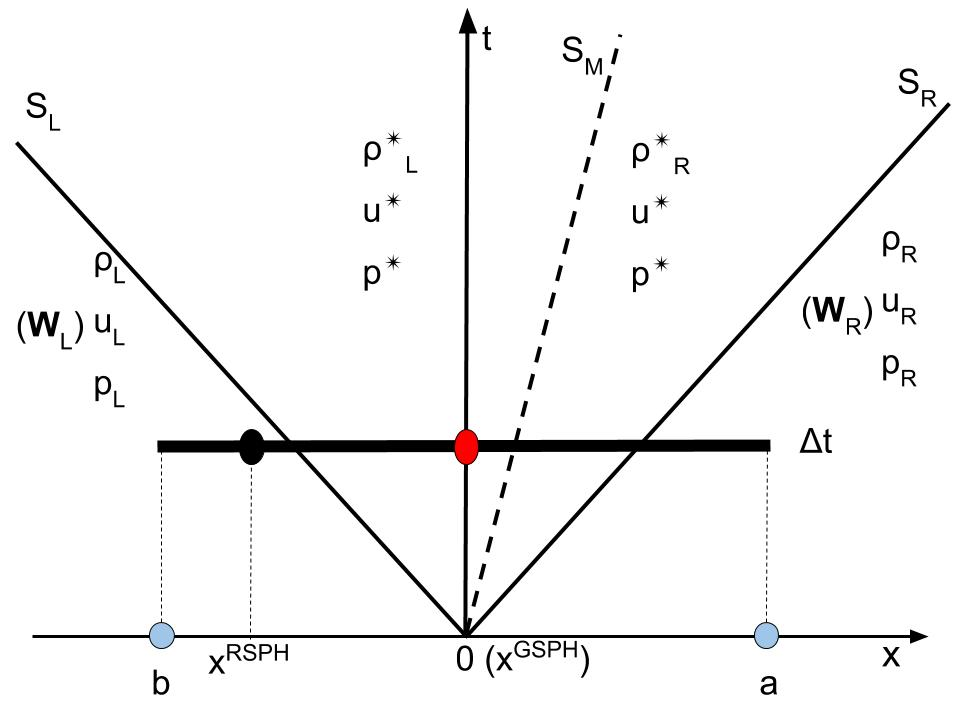
\includegraphics[width=0.5 \textwidth]{./Figures/RSPH-GSPH}
    \caption{Evaluating of the starred state for  RSPH and GSPH implementations. $x$ is the local coordinate system for paired two particles, $a$ and $b$. The origin is at the middle of the paired two particles.
The the local Riemann problem is defined by the constant states $(\rho, u, p)_a$ and $(\rho, u,p)_b$, namely $\textbf{W}_L = \textbf{W}_b$, $\textbf{W}_R = \textbf{W}_a$ with $\textbf{W} = (\rho, u,p)^T $, a vector representation of these three variables. The horizontal bold solid line at time $\Delta t$ indicates the interval on which to evaluate the solution of the Riemann problem. The dark ellipse is an example sample point of RSPH with the random number. The red ellipse indicates the stationary state, which is the starred state in GSPH. $S_L$, $S_M$ and $S_R$ are singal speeds which are linerized locally in HLLC Riemann solvers \citep{puri2014approximate}. Starred region is divided into two sub-regions by the middle contact wave. Only $\rho$ changes across the contact wave. }
    \label{fig:pick-up-state-GSPH-RSPH}
\end{figure}

The starred state $(u^{\ast},  p^{\ast})$ must now be projected back into the global coordinate system, to define  $(\textbf{v}^{\ast},  p^{\ast})$.

We mention that, instead of selecting a uniformly distributed random number $\epsilon$, we follow \citet{colella1982glimm} and adopt the Van Der Corput pseudo-random number sequence \citep{hammersley2013monte}.

\subsection{Non-iterative Riemann solvers} \label{sec:RP-solver}
Solving local Riemann problems exactly usually involves separating several cases of wave patterns and iteratively solving a small system of ordinary differential equations (for rarefaction waves) and a small set of nonlinear equations (the Rankine-Hugoniot equations). Instead of running this lengthy process one can employ approximate Riemann solvers, which provide an approximate solution quickly. There are many approximate Riemann solvers available \citep{rider1994review, luo2004computation, puri2014approximate}. For purposes here we adopt the HLLC solver, which decomposes the Riemann solution into 3 waves, including a (possible) contact discontinuity \cite{toro1994restoration}. More specifically, we adopt the HLLC formulation proposed by \citet{luo2004computation}.
 
We mention that, in the numerical tests in Section \ref{numericaltests}, Both the HLLC solver and Roe solver are used for GSPH calculations.
To summarize, our RSPH algorithm proceeds as follows:
\begin{itemize}
\item For each pair of particles, establish a local coordinate system whose axis joins the particles,
and project the primitive variables onto this local coordinate system to define left and right states;
\item Solve this local Riemann problem approximately using a HLLC solver;
\item Sample the solution using the Van Der Corput sequence, defining a state  $p^{\ast}, u^{\ast}$;
\item Project $p^{\ast}, u^{\ast}$  back to the global coordinate system, to obtain $p^{\ast}$ and $\textbf{v}^{\ast}$;
\item Update the particle positions and physical quantities.
\end{itemize}

\section{Numerical tests} \label{numericaltests}
We describe results from several numerical tests using SPH, RSPH and GSPH in this section.
A 1D shock tube test is used to compare standard SPH, GSPH and RSPH. More shock tube simulations are also conducted to check the capacity of RSPH for different situations. In addition, order of accuracy is investigated for the 1D shock tube problem. In the last subsection we describe a 3D free jet flow simulation with SPH, GSPH and RSPH to check equivalent overall dissipation introduced by each method.

Six 1D simulations described here are carried out:
\begin{itemize}% [1D Tests]
\item Test 1 consists of a left rarefaction, a right traveling contact and a right shock. Density increases at down wind of contact wave. 
\item Test 2 also consists of a left rarefaction, a right traveling contact and a right shock. Density decreases at down wind of contact wave. 
\item Test 3 includes double expansion waves. The initial density is different at right and left hand side. 
\item Test 4 is a double shock test with different initial densities on the right side and left side.
\item Test 5 and Test 6 are two extreme cases. Test 5 is a cavity flow while test 6 is a strong blast flow.
\end{itemize}

\begin{table}[H]
\centering
      \caption{Overview of 1D shock tube tests}		
	  \begin{tabular}{lrrrrrrrrrr}
	    \hline
	          & $\rho_L$ & $p_L$ &$v_L$ & $\rho_R$ & $p_R$ &$v_R$ & $m$ & $[x_L, x_R]$ & $t_f$\\
	    \hline
	    Test 1 & $1.0$ & $1.0$ &$0$ & $0.25$ & $0.1795$ &$0$ & $0.003$  & $[-0.4, 0.4]$ & $0.17$\\
	    	Test 2 & $1.0$ & $1.0$ &$0$ & $0.5$ & $0.2$ &$0$ & $0.003$  & $[-0.4, 0.4]$ & $0.2$\\
	    	Test 3 & $2.0$ & $1.95$ &$-1.0$ & $1.0$ & $1.95$ &$1.0$  & $0.006$  & $[-0.4, 0.4]$ & $0.13$\\
	    Test 4 & $1.0$ & $2.4$ &$8.0$ & $0.5$ & $0.4$ &$-0.25$ & $0.003$  & $[-0.4, 0.4]$ & $0.05$\\
	    	Test 5 & $1.0$ & $0.4$ &$-2.0$ & $1.0$ & $0.4$ &$2.0$ & $0.003$  & $[-0.4, 0.4]$ & $0.18$\\
	    	Test 6 & $1.0$ & $1000$ &$0$ & $1.0$ & $0.01$ &$0$ & $0.003$  & $[-0.5, 0.5]$  & $0.01$\\
	    \hline
	  \end{tabular}
	  \label{tab:1D-shock-input_parameters}
\end{table}
Input parameters for 1D tests can be found in Table \ref{tab:1D-shock-input_parameters}, where, subscript $L$ refers left side and $R$ for right side. $m$ is particle mass, initial interval between adjacent particles are adjusted to guarantee equal particle mass. $t_f$ is the time to terminate simulation and plotting the results. Equal particle mass is assigned to all particles. The $x$ axis in all plots is normalized by time, that is $x/t_f$, in plots for shock tube tests results.
\subsection{Comparison of RSPH with standard SPH and GSPH}
\begin{figure}[H]
    \centering
    \begin{minipage}{.495\textwidth}
        \centering a)
        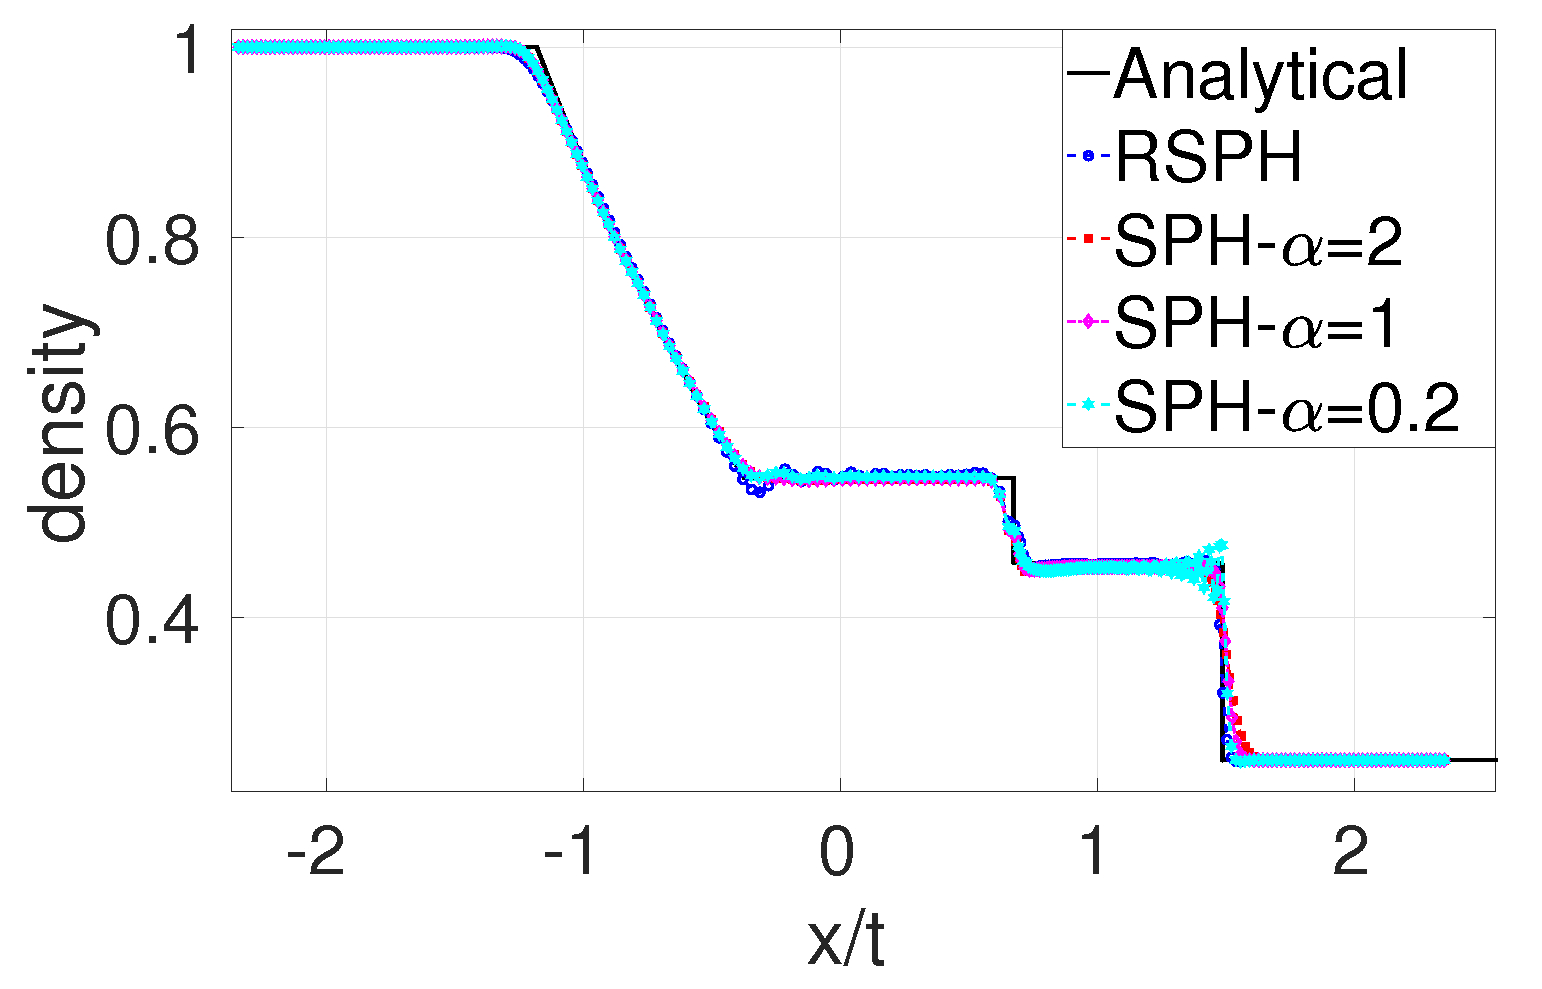
\includegraphics[width=0.99 \textwidth,height=0.7\textwidth]{./Figures/RCM-Sod-SPH-alf-rho}
    \end{minipage}%
    \begin{minipage}{.495 \textwidth}
        \centering b)
        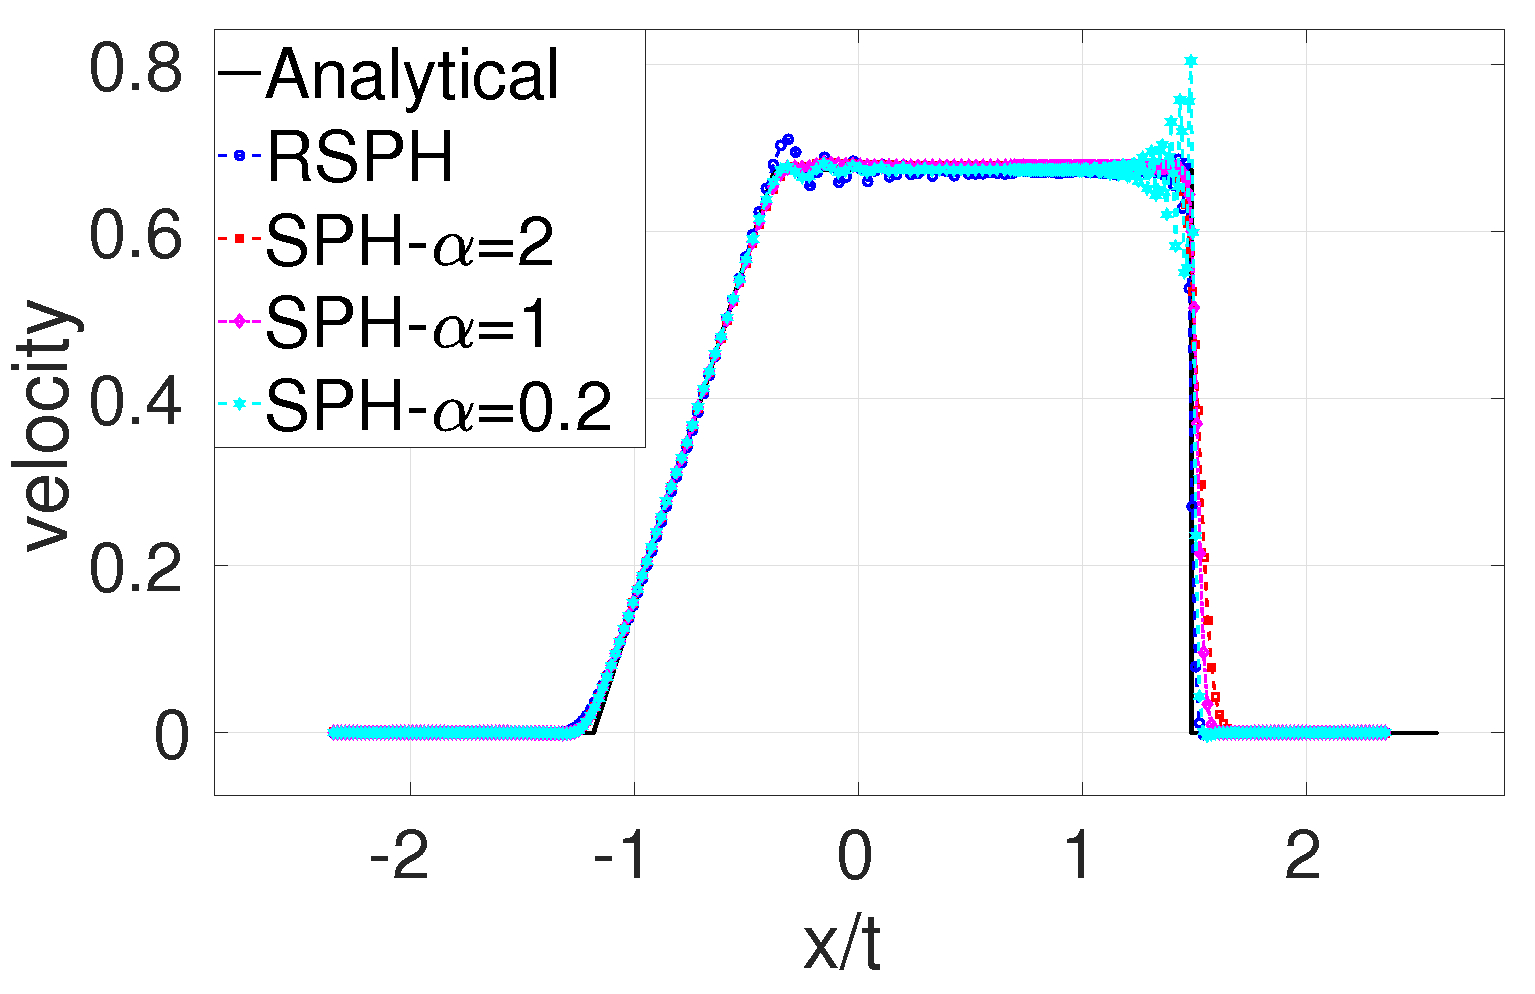
\includegraphics[width=0.99 \textwidth,height=0.7\textwidth]{./Figures/RCM-Sod-SPH-alf-v}
    \end{minipage}%
    \\
    \begin{minipage}{.495\textwidth}
        \centering c)
        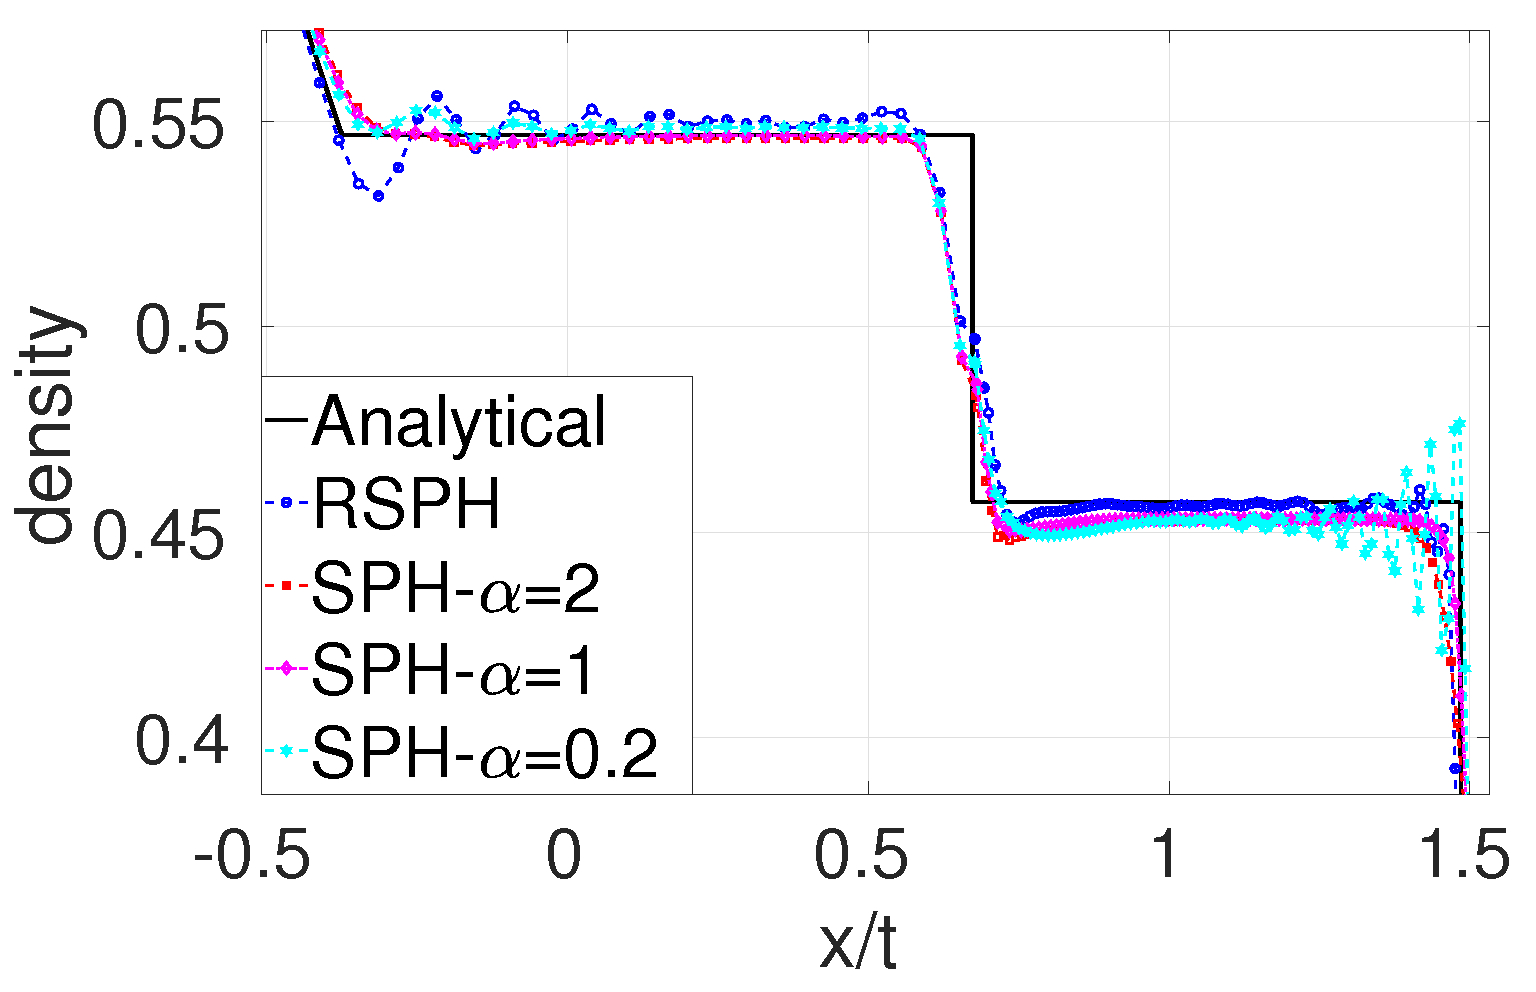
\includegraphics[width=0.99 \textwidth,height=0.7\textwidth]{./Figures/RCM-Sod-SPH-alf-rho-zoom}
    \end{minipage}%
    \begin{minipage}{.495 \textwidth}
        \centering d)
        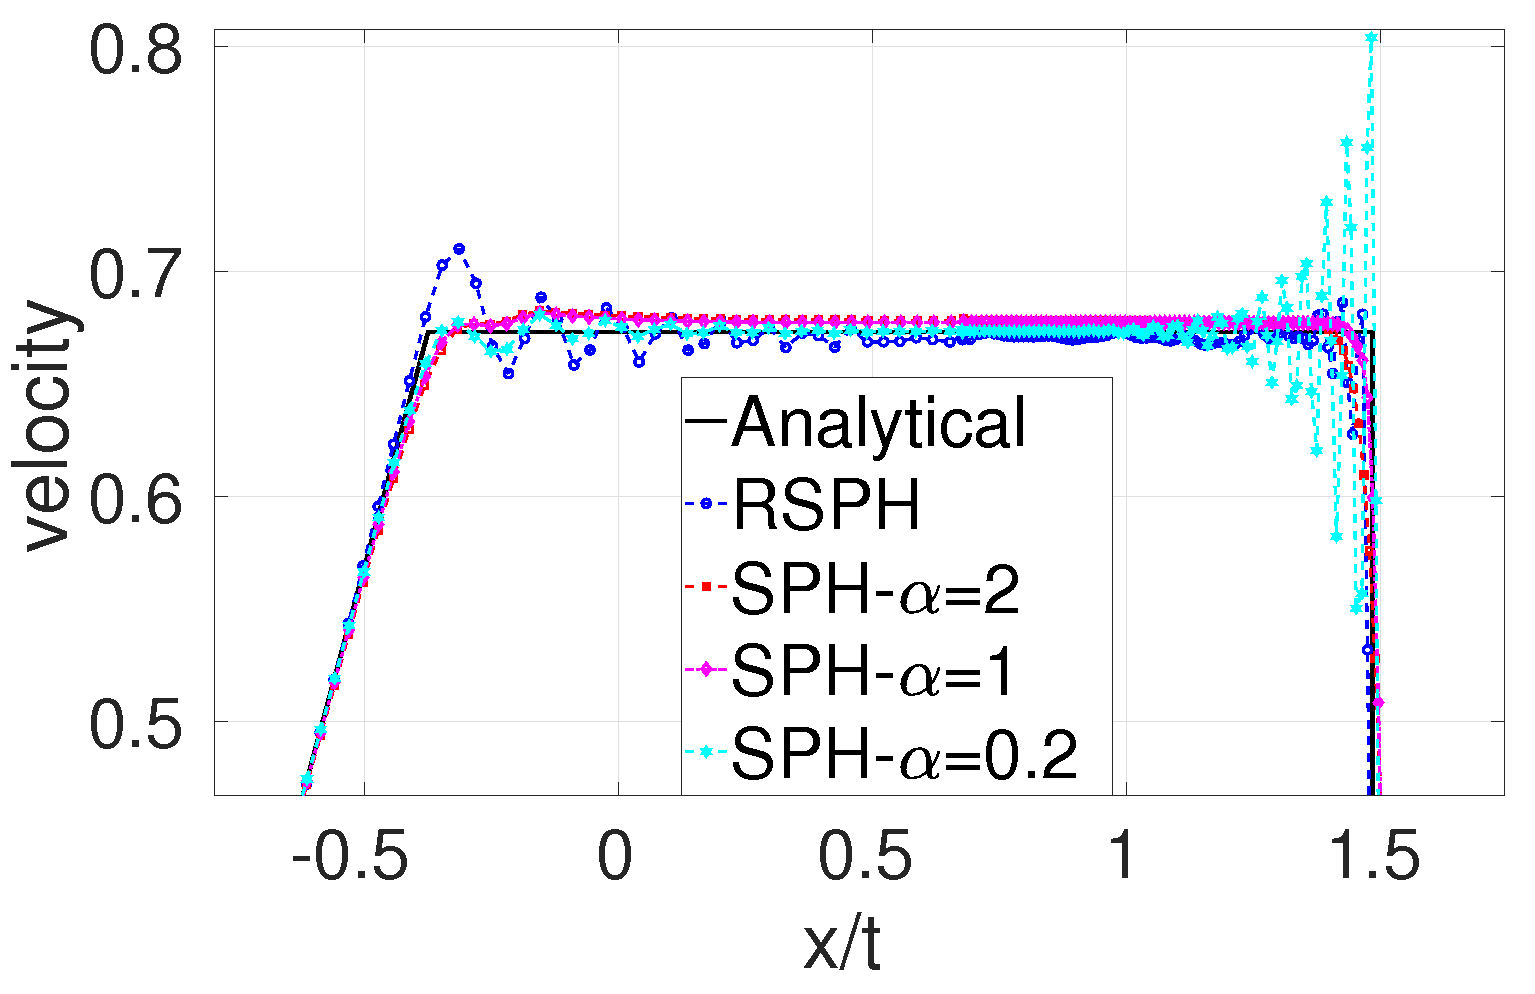
\includegraphics[width=0.99 \textwidth,height=0.7\textwidth]{./Figures/RCM-Sod-SPH-alf-v-zoom}
    \end{minipage}%   
    \caption{a),b) are simulation results of density and velocity in Test 1 by RSPH and SPH with different artificial viscosity coefficients $\alpha,\beta$ satisfying: $\beta=2\alpha$.  c), d) are zoomed views, showing that $\alpha=0.2$ provided insufficient viscosity to suppress oscillations around shock. The dissipation introduced by RSPH. on the other hand, is adaptive, introducing more damping at the shock (comparable to $\alpha=1.0$) and less damping in the area away from the shock (less than $\alpha=0.2$, as indicated by the magnitude of oscillation).}
    \label{fig:RCM-Sod-SPH-alf}
\end{figure}

\begin{figure}[H]
    \centering
    \begin{minipage}{.495\textwidth}
        \centering a)
        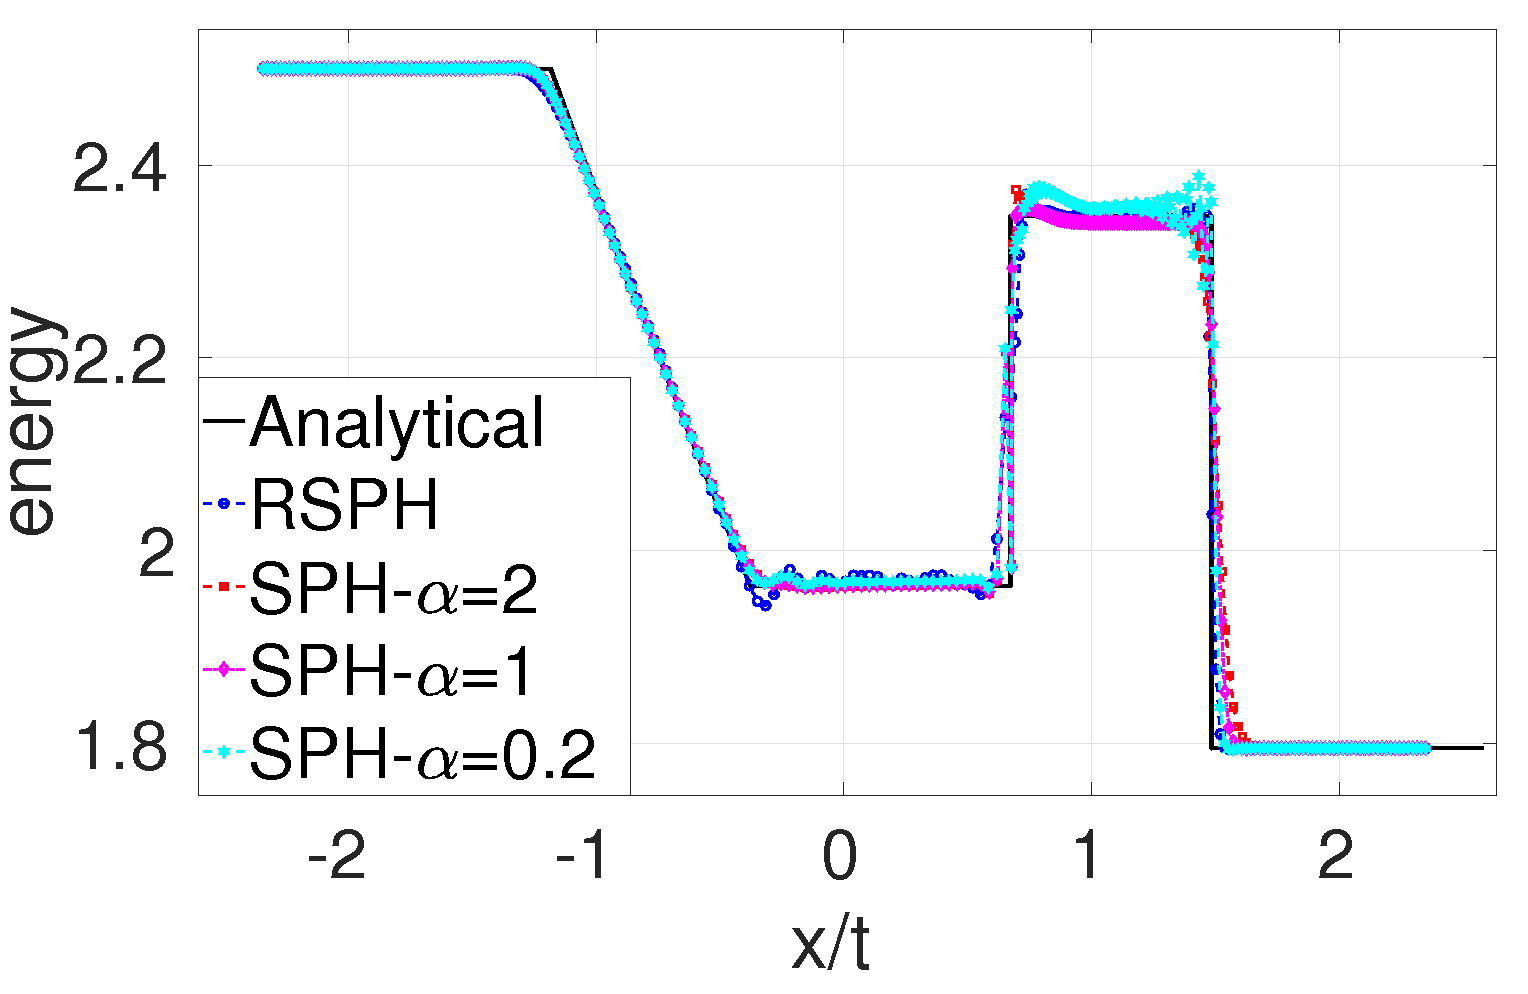
\includegraphics[width=0.99 \textwidth,height=0.7\textwidth]{./Figures/RCM-Sod-SPH-alf-e}
    \end{minipage}%
    \begin{minipage}{.495 \textwidth}
        \centering b)
        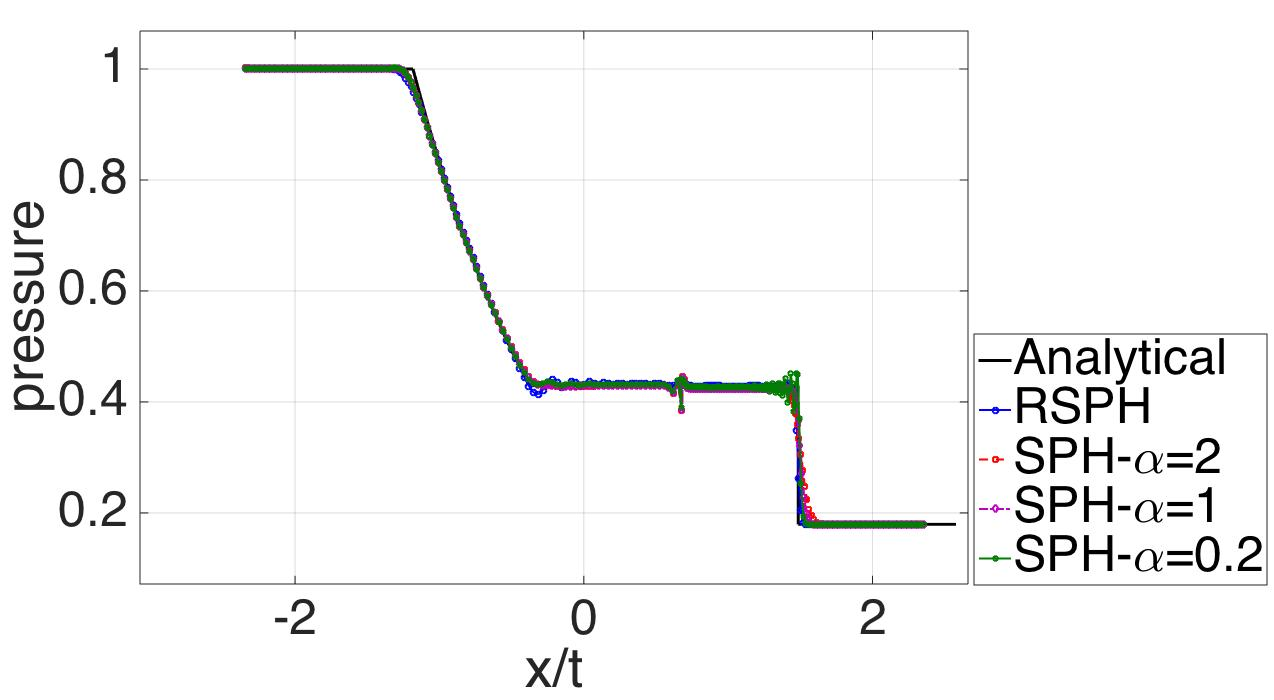
\includegraphics[width=0.99 \textwidth,height=0.7\textwidth]{./Figures/RCM-Sod-SPH-alf-p}
    \end{minipage}% 
    \\
    \begin{minipage}{.495 \textwidth}
        \centering c)
        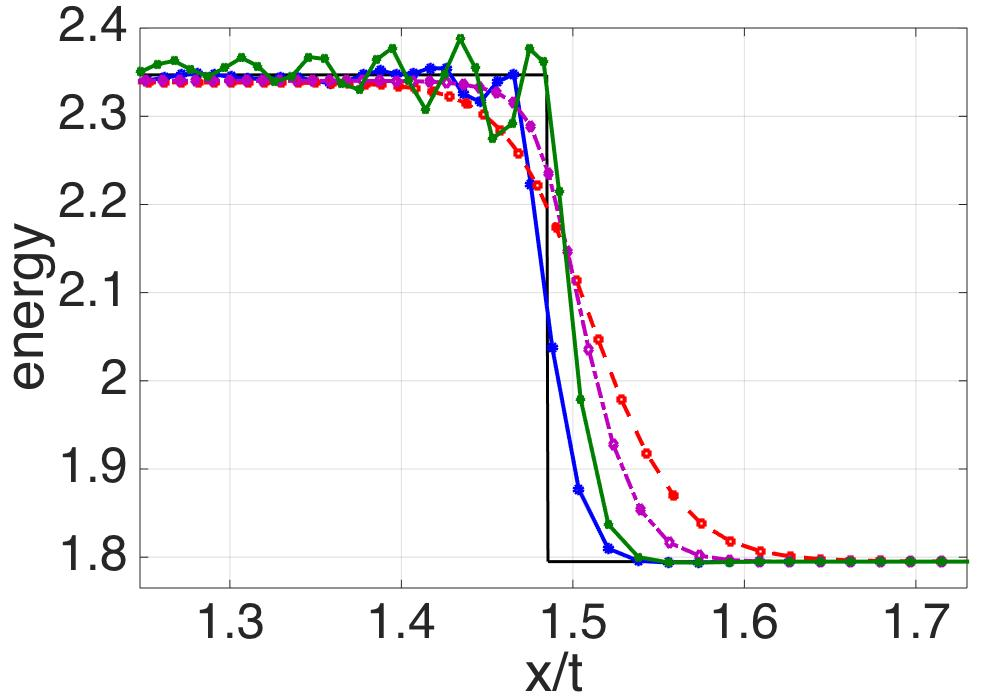
\includegraphics[width=0.99 \textwidth, height=0.7\textwidth]{./Figures/RCM-Sod-SPH-alf-e-zoom}
    \end{minipage}% 
    \begin{minipage}{.495\textwidth}
        \centering d)
        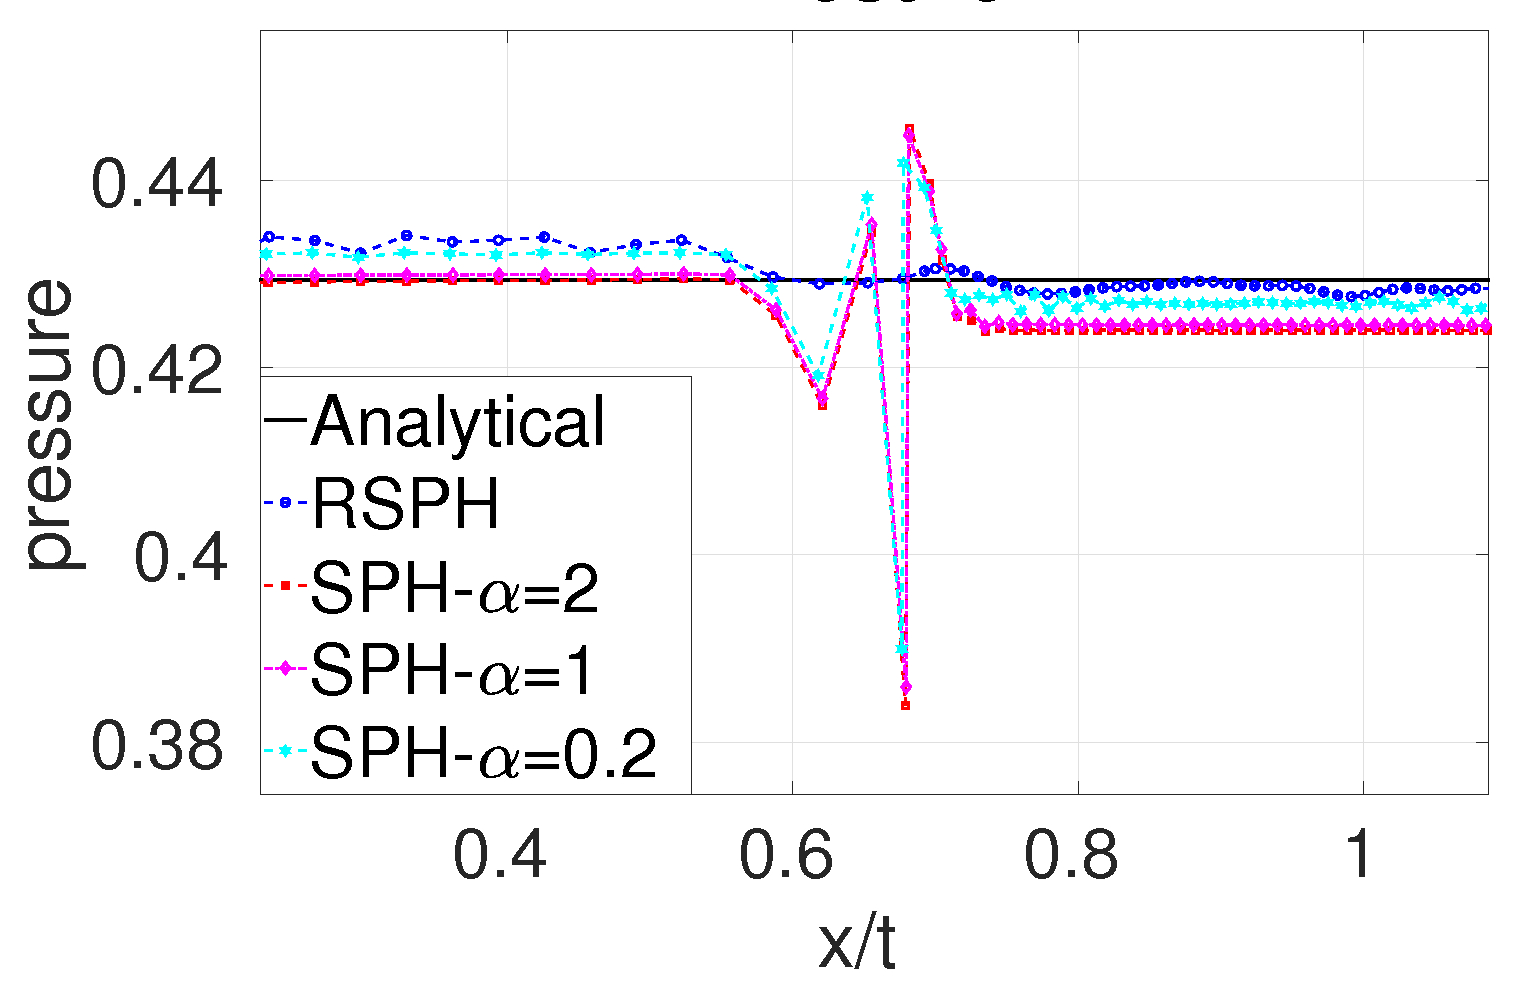
\includegraphics[width=0.99 \textwidth, height=0.7\textwidth]{./Figures/RCM-Sod-SPH-alf-p-zoom}
    \end{minipage}%    
    \caption{
    a),b) are simulation results of internal energy and pressure in Test 1 by RSPH and SPH with different artificial viscosity coefficients $\alpha,\beta$ satisfying: $\beta=2\alpha$.  c), d) are zoomed views.  For $\alpha=1$ and $\alpha=2$, as shown in c), numerical oscillations are completely suppressed though the shock is now smeared. $\alpha=0.2$ provided insufficient viscosity to suppress oscillations. Comparing RSPH and SPH shows that RSPH is adaptive, more dissipative at the shock (comparable or better than $\alpha=1.0$) and less dissipative away from the shock (less than $\alpha=0.2$). d) shows pressure around the contact discontinuity. It is evident that RSPH gets rid of the pressure ``wiggle" around the contact discontinuity.}
    \label{fig:RCM-Sod-SPH-alf-zoom}
\end{figure}

Test 1 is simulated using standard SPH with different artificial viscosity coefficients, GSPH and RSPH. The comparison between RSPH and SPH using different artificial viscosity coefficients is shown in Fig. \ref{fig:RCM-Sod-SPH-alf} and \ref{fig:RCM-Sod-SPH-alf-zoom}. In all simulations, the artificial viscosity coefficient $\beta$ is set to be twice of $\alpha$. For example, for the test ``$SPH-\alpha=2$", $\beta=4$. Several interesting observation are made based on the comparison between SPH and RSPH. The effect of artificial viscosity is illustrated through comparison.
First of all, dissipation (introduced by artificial viscosity in these tests) decays the numerical fluctuations. Numerical fluctuations are suppressed completely when large enough dissipation is introduced, for example, by using sufficiently large artificial viscosity coefficients ($\alpha=1,2$).
Secondly, the equivalent artificial viscosity introduced by RSPH varies adaptively.
As shown in Fig. \ref{fig:RCM-Sod-SPH-alf} and \ref{fig:RCM-Sod-SPH-alf-zoom}, RSPH assigns smaller artificial viscosity  (equivalent $\alpha$ much less then 0.2) at the area far away from shock and sufficiently large artificial viscosity coefficients (equivalent $\alpha$ is about 1.0) around the shock. So RSPH is actually more adaptive than SPH. This feature is very desirable not only because it could eliminate parameterization and hence user intervention associated with artificial viscosity coefficients but also because it avoids introducing excess artificial viscosity.
Thirdly, RSPH introduces less smearing of the shock discontinuity compared with SPH using most commonly adopted artificial viscosity coefficients ($\alpha=1.0$, $\beta=2.0$). Recall that RCM is able to resolve discontinuities as true discontinuity. RSPH, even though it still smears the discontinuity in some degree, introduces much less smearing (see Fig. \ref{fig:RCM-Sod-SPH-alf-zoom}).
The last but not the least, the pressure ``wiggle" around contact discontinuity is completely eliminated by RSPH as seen in Fig. \ref{fig:RCM-Sod-SPH-alf-zoom}. It has been shown that thermal conduction is essential to mitigate the spurious pressure ``wiggle" at contact discontinuity in SPH \citep{monaghan1997sph, sigalotti2006shock, price2008modelling, price2012smoothed}. As for GSPH, it is reported that an implicit thermal conduction is introduced by Godunov's scheme and helps suppress the anomaly \citep{puri2014approximate}. Even though, the ``wiggle" still visible in pressure distribution and velocity distribution of GSPH simulation results (for example, see figures in \citep{puri2014comparison}) and RSPH simulation results of other tests (see section \ref{sec:comprehensive-1d-tests}). ``Wiggle" in test 1, however, is completely eliminated by both GSPH and RSPH.

\begin{figure}[H]
    \centering
    \begin{minipage}{.495\textwidth}
        \centering
        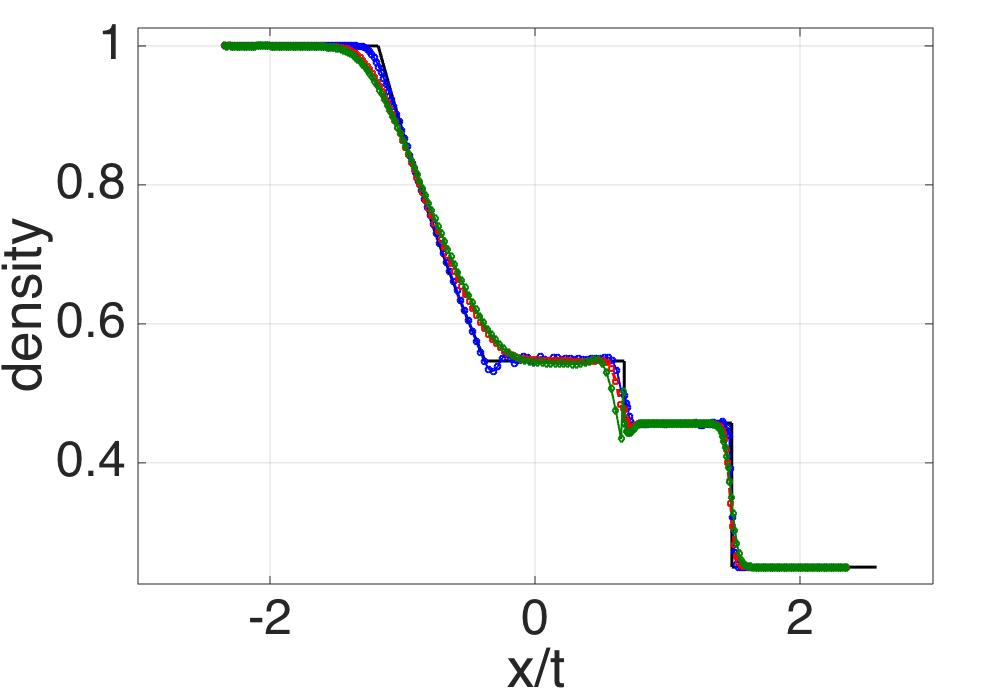
\includegraphics[width=0.99 \textwidth,height=0.6\textwidth]{./Figures/RCM-Sod-GSPH-compare-rho}
    \end{minipage}%
    \begin{minipage}{.495 \textwidth}
        \centering
        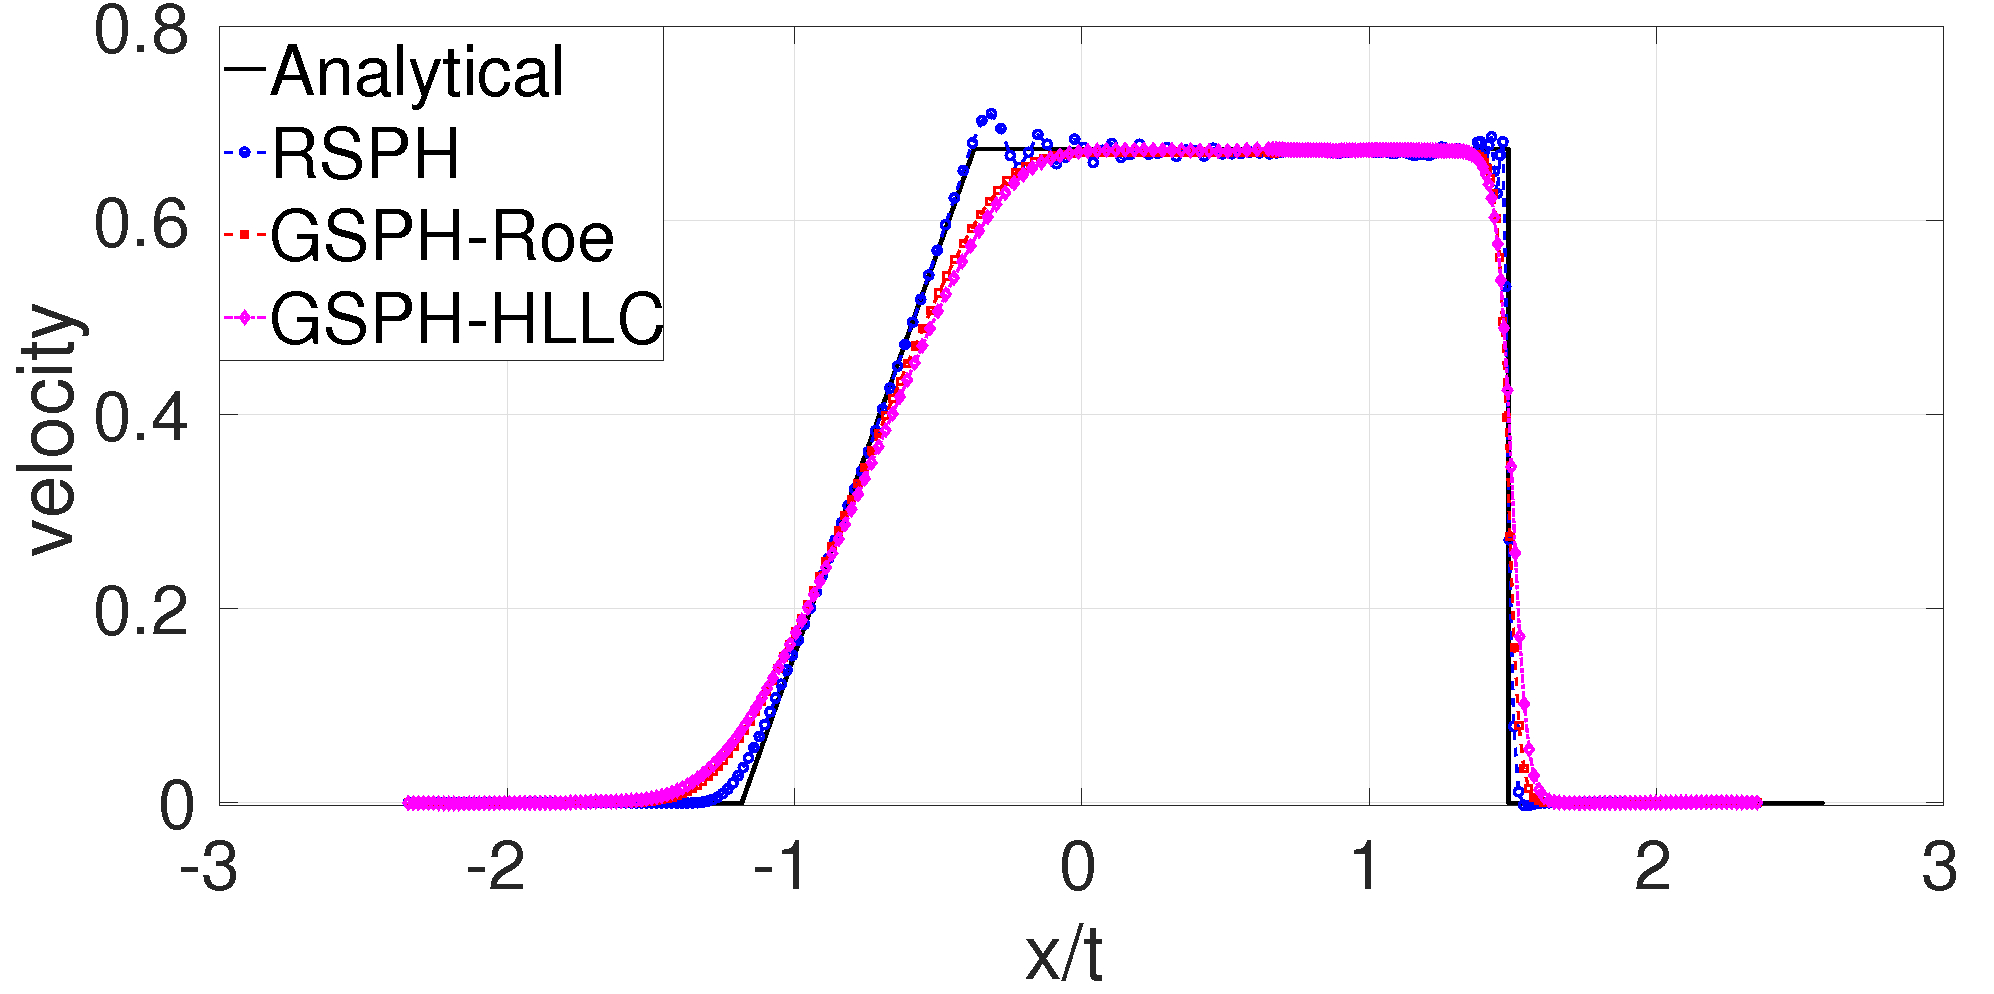
\includegraphics[width=0.99 \textwidth,height=0.6\textwidth]{./Figures/RCM-Sod-GSPH-compare-v}
    \end{minipage}%
    \\
    \begin{minipage}{.495\textwidth}
        \centering
        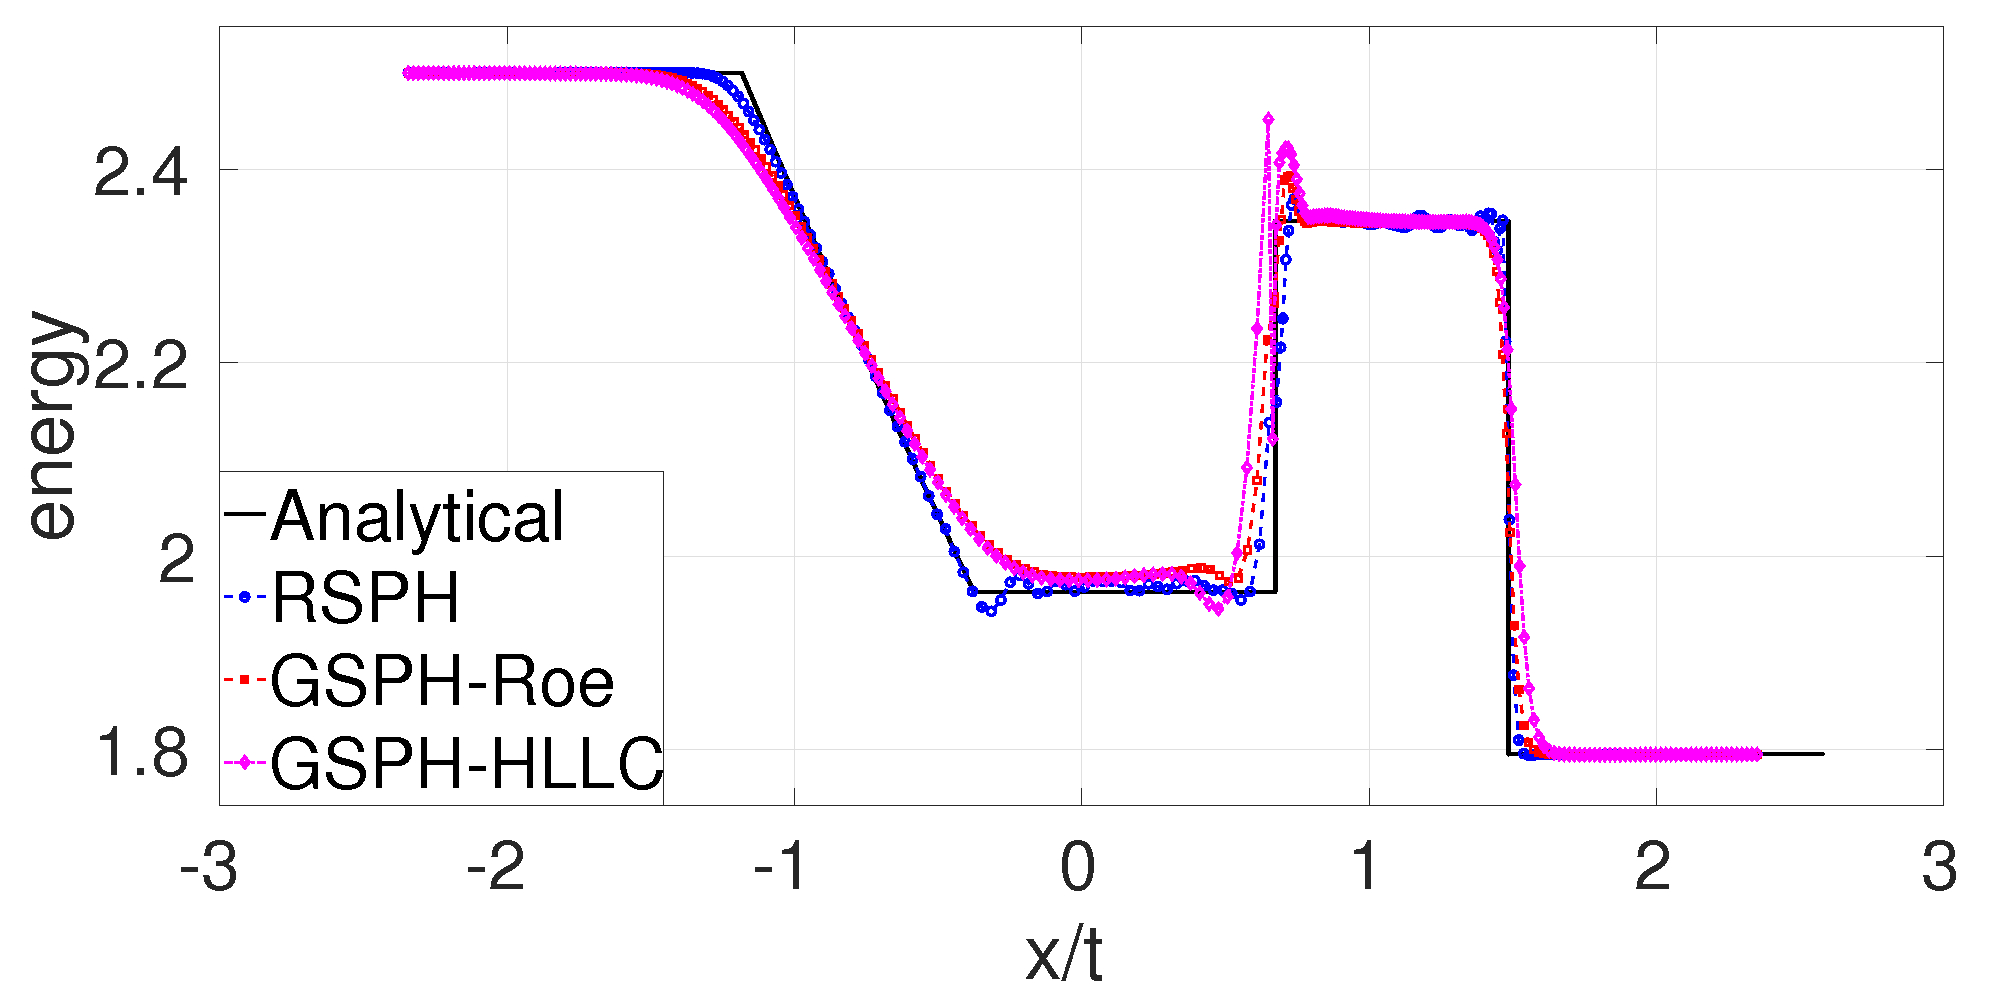
\includegraphics[width=0.99 \textwidth,height=0.6\textwidth]{./Figures/RCM-Sod-GSPH-compare-e}
    \end{minipage}%
    \begin{minipage}{.495 \textwidth}
        \centering
        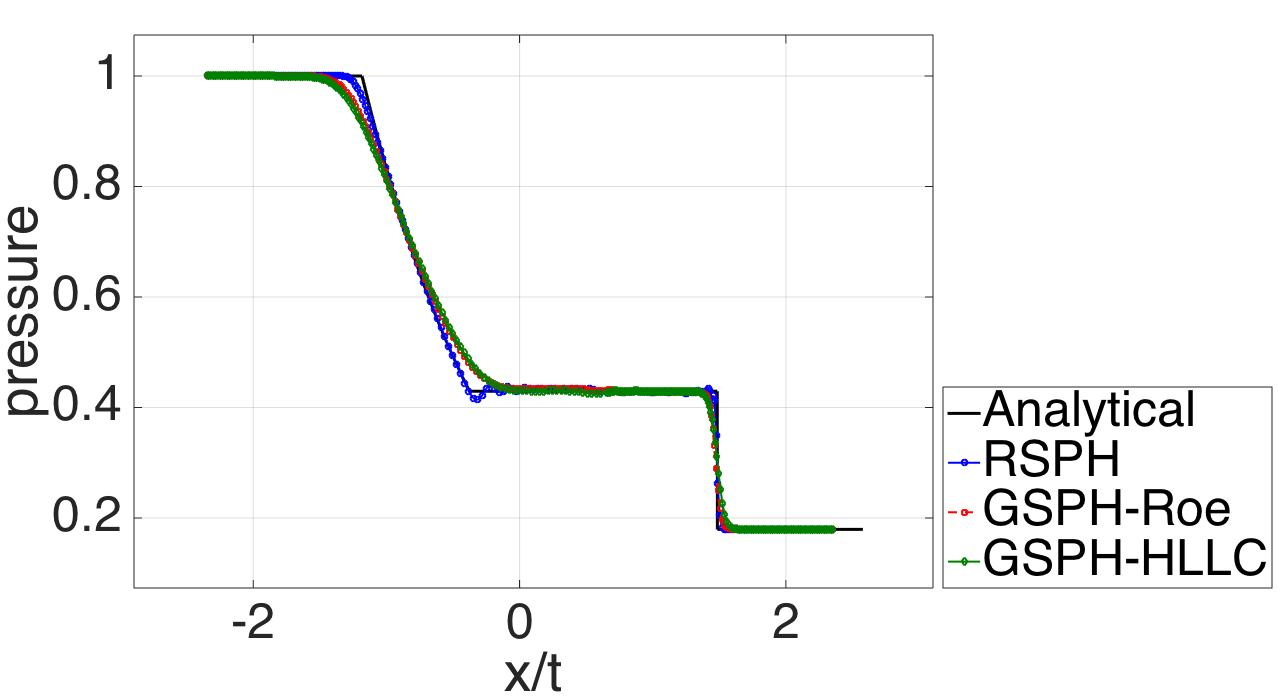
\includegraphics[width=0.99 \textwidth,height=0.6\textwidth]{./Figures/RCM-Sod-GSPH-compare-p}
    \end{minipage}% 
    \\
    \begin{minipage}{.495\textwidth}
        \centering
        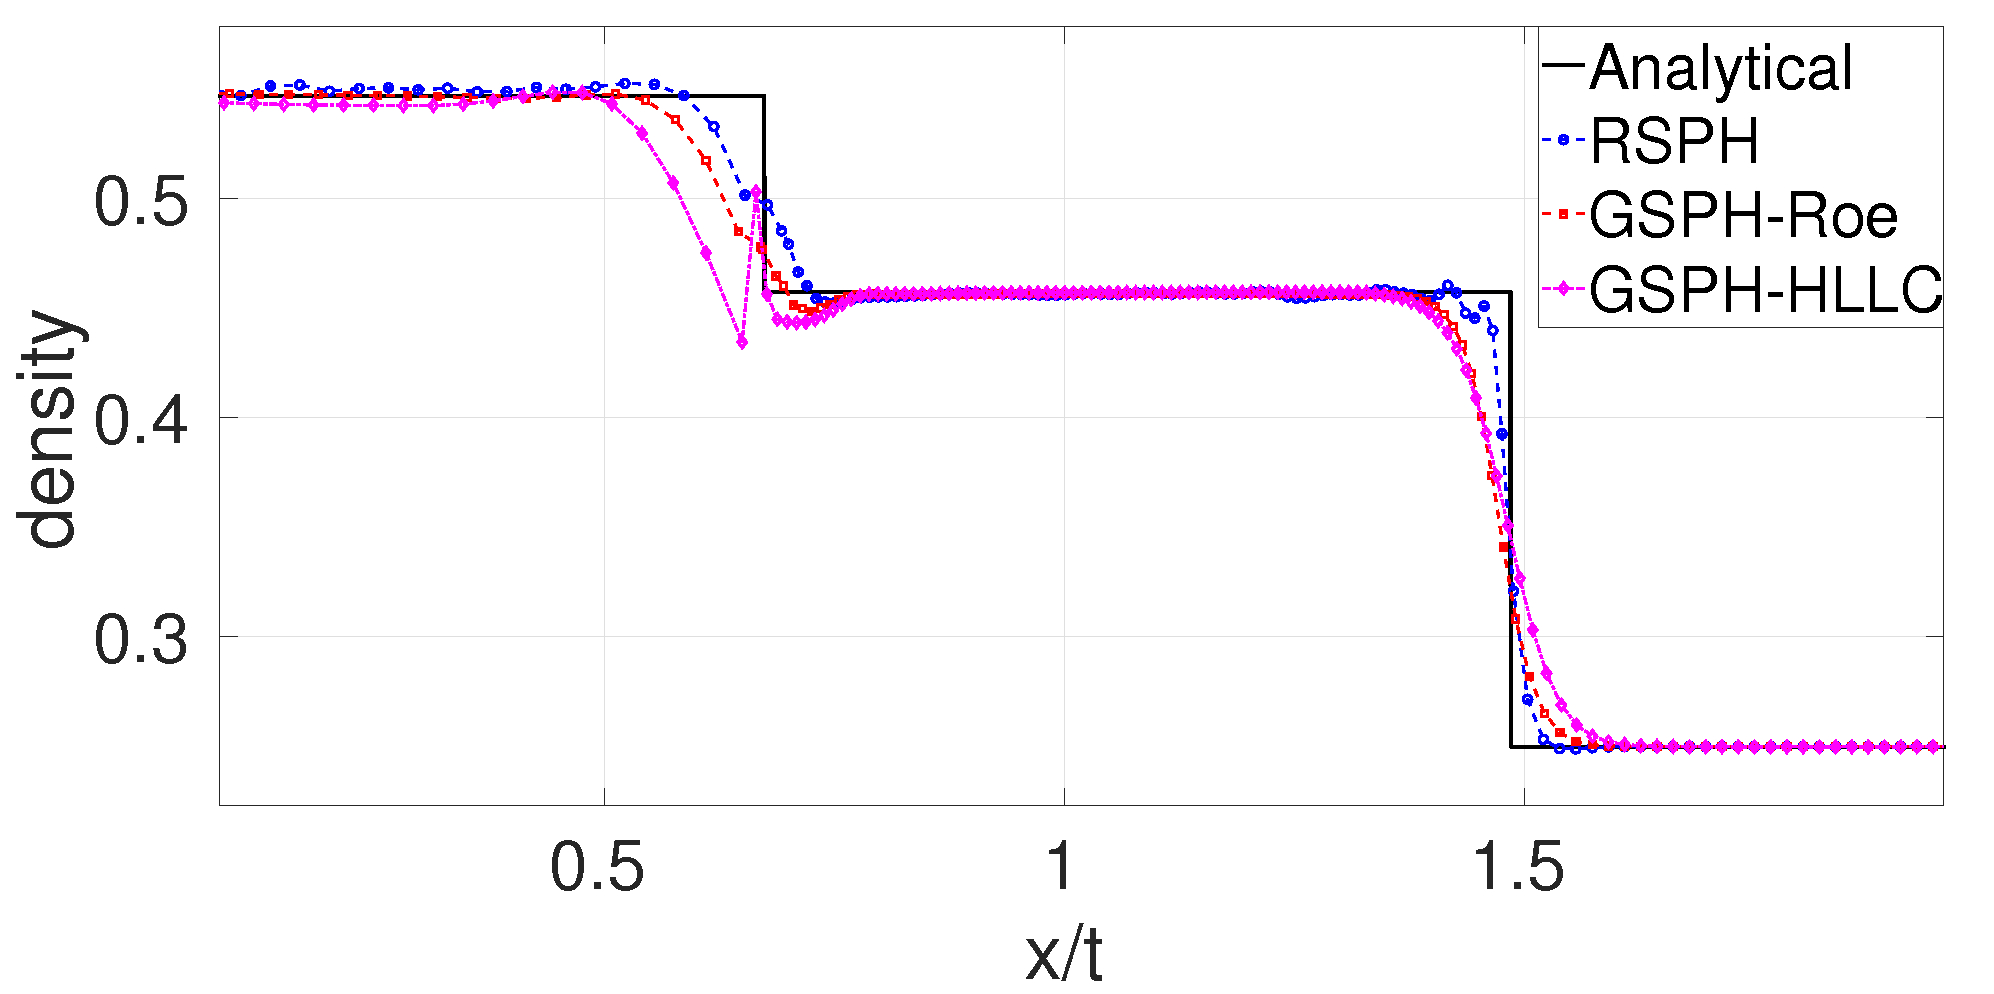
\includegraphics[width=0.99 \textwidth,height=0.6\textwidth]{./Figures/RCM-Sod-GSPH-compare-rho-zoom}
    \end{minipage}%
    \begin{minipage}{.495 \textwidth}
        \centering
        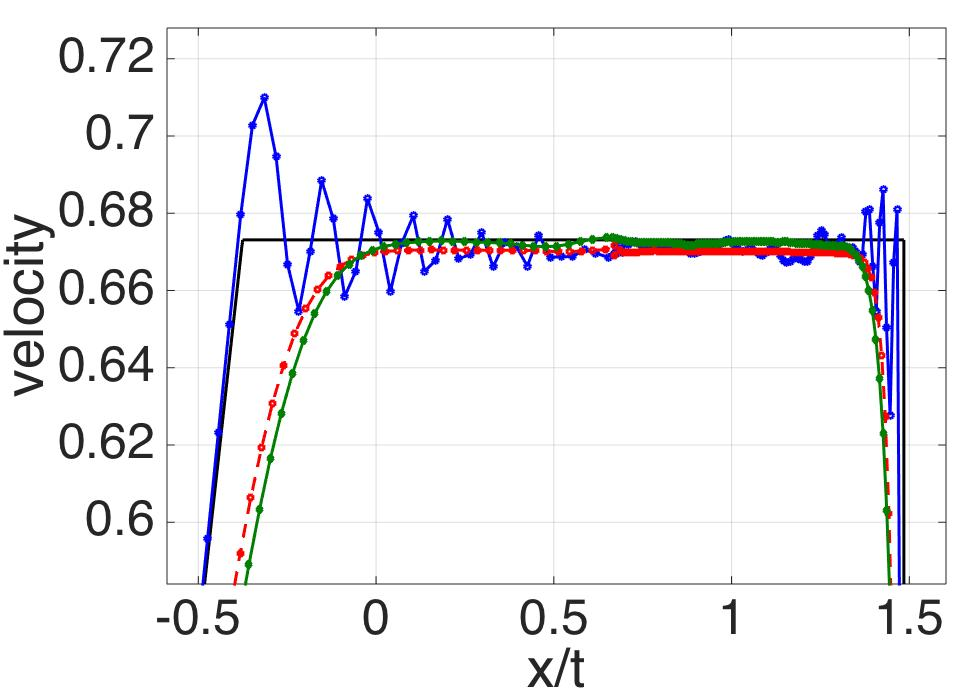
\includegraphics[width=0.99 \textwidth,height=0.6\textwidth]{./Figures/RCM-Sod-GSPH-compare-v-zoom}
    \end{minipage}% 
       \\
    \begin{minipage}{.495 \textwidth}
        \centering
        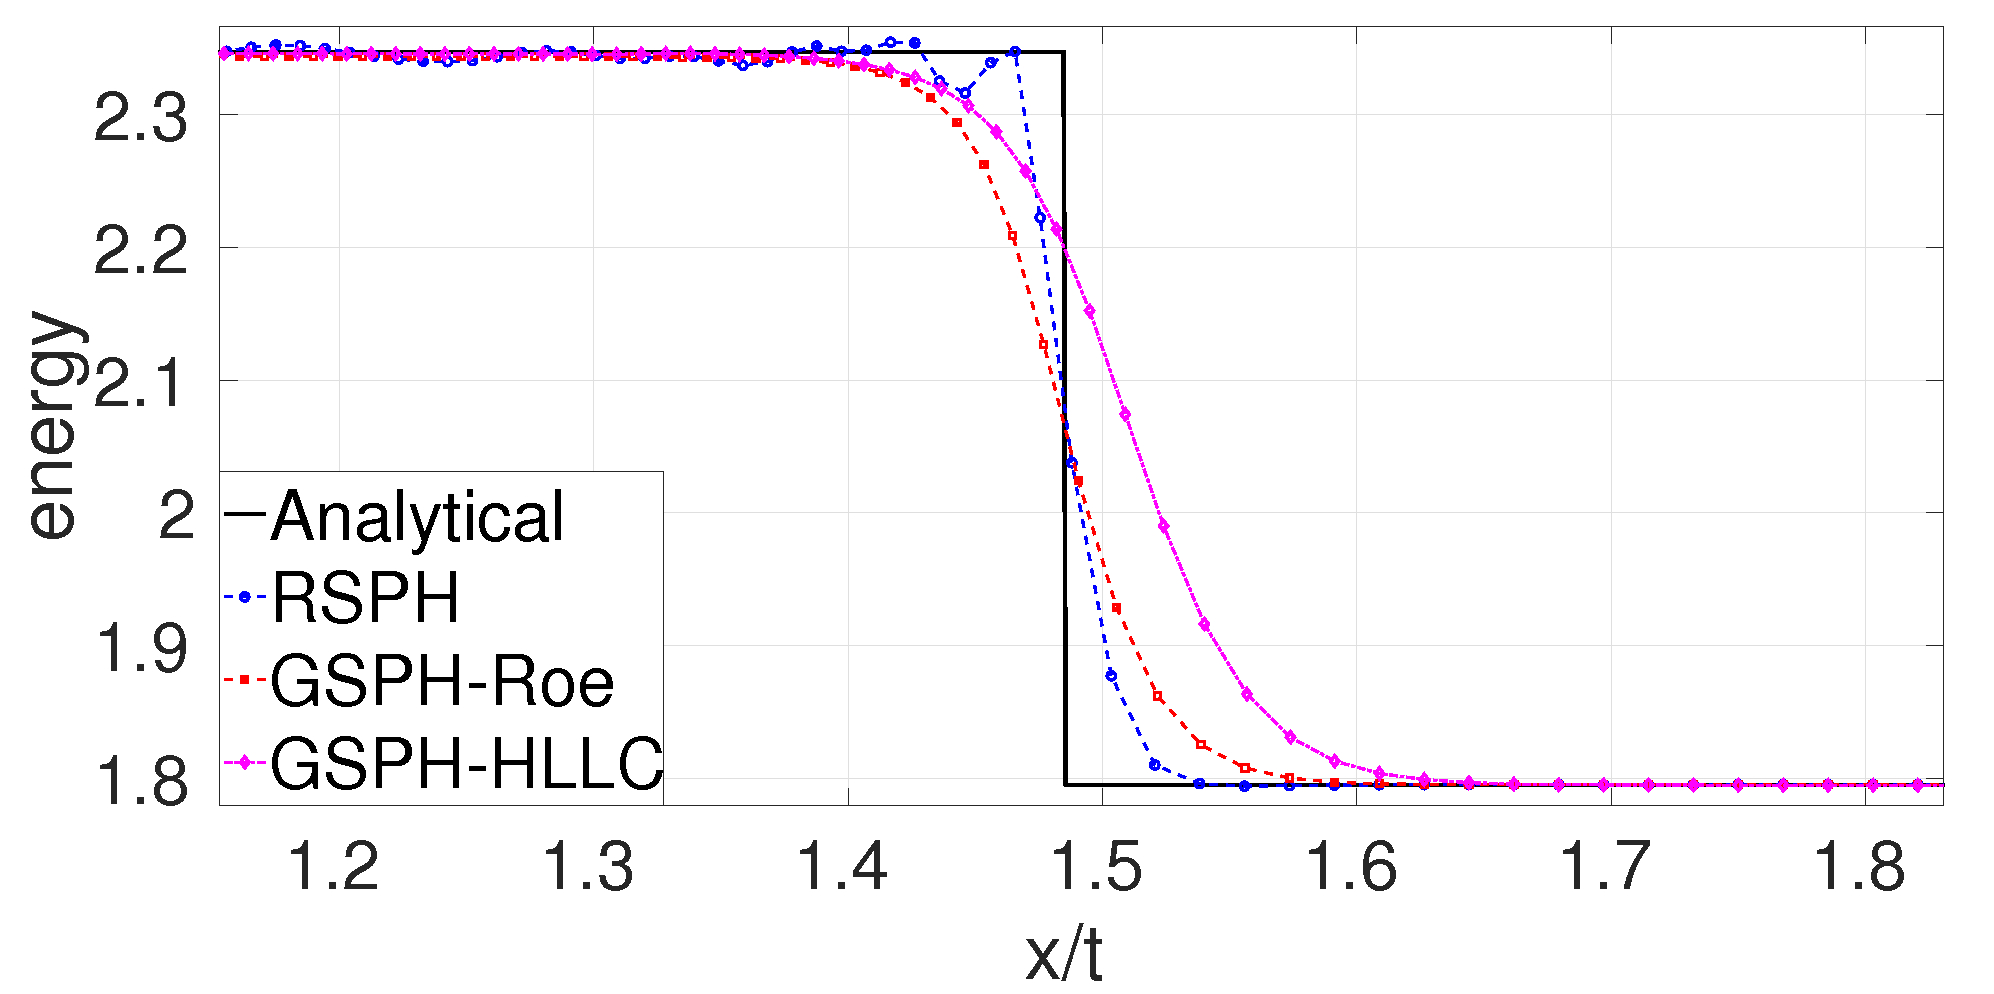
\includegraphics[width=0.99 \textwidth,height=0.6\textwidth]{./Figures/RCM-Sod-GSPH-compare-e-zoom}
    \end{minipage}% 
    \begin{minipage}{.495\textwidth}
        \centering
        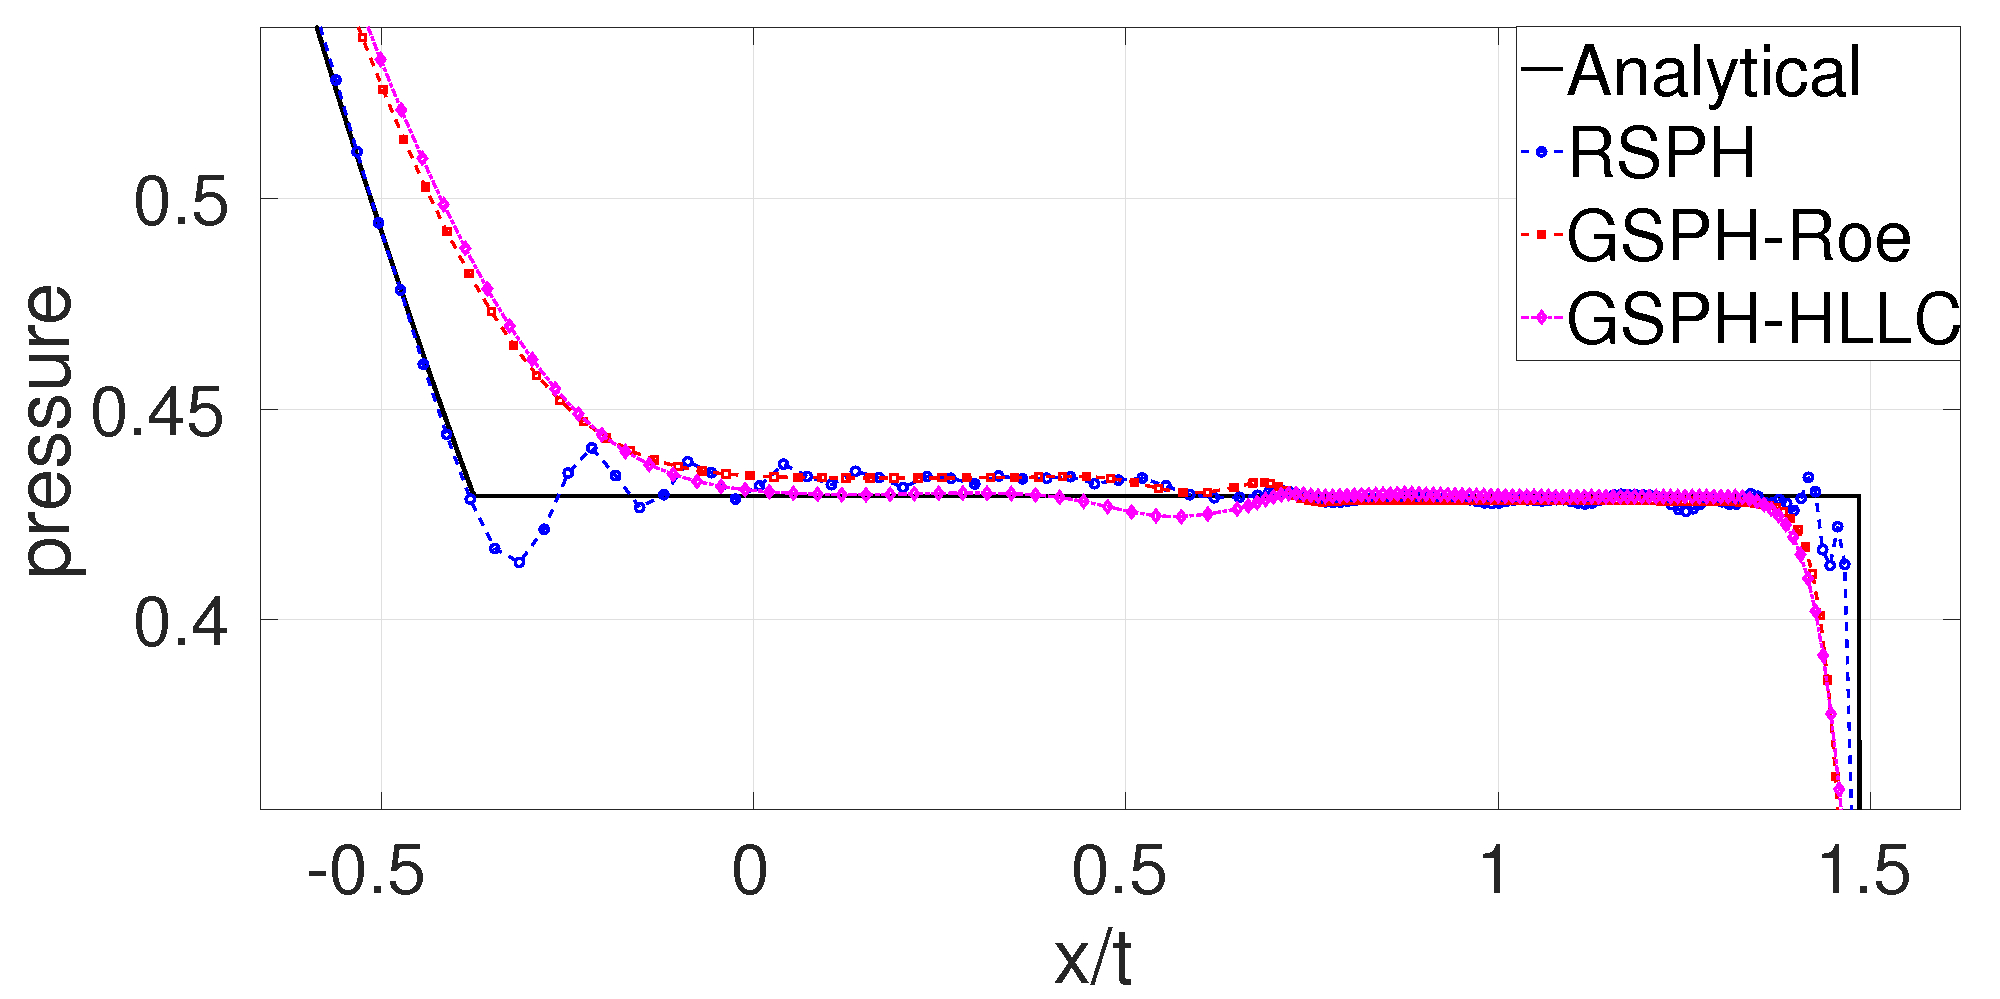
\includegraphics[width=0.99 \textwidth,height=0.6\textwidth]{./Figures/RCM-Sod-GSPH-compare-p-zoom}
    \end{minipage}%    
    \caption{Comparison of RSPH with GSPH using Roe Riemann solver and HLLC Riemann solver. The last four plots are zoomed views. Zoomed view of density and specific internal energy show that GSPH smears the discontinuity at shock much more than RSPH. Zoomed view of velocity shows that fluctuation in GSPH is completely suppressed, which implies that numerical dissipation introduced in GSPH is at least around the same amount as SPH with $\alpha=1.0$. This is consistent with information implied by zoomed view of density and specific internal energy. The last zoomed view shows that both RSPH and GSPH can get rid of pressure ``wiggle" around the contact discontinuity.}
    \label{fig:RCM-Sod-GSPH}
\end{figure}

Zoomed views in Fig. \ref{fig:RCM-Sod-GSPH} compare GSPH and RSPH and demonstrate that RSPH introduces less but sufficient dissipation compared with GSPH. The attractive feature of RCM method in preserving true discontinuity is inherited by RSPH in this 1D shock tube test. With more numerical dissipation, GSPH can completely suppress numerical oscillations. However, the discontinuity at the shock is then more seriously smeared. The excessive amount of dissipation might have other, more undesirable, effects in real implementation. For example, over damping of shearing flow. Compared with SPH, both GSPH and RSPH avoid pressure ``wiggle" around contact discontinuity. Since RSPH shares many commonalities   with Godunov's method, it is not a surprise that RSPH can also suppress the pressure ``wiggle" at contact discontinuity.

\subsection{Accuracy tests}
We use shock tube test to gauge the accuracy of the RSPH scheme.
We examine the errors between simulation results and the analytical solution (the reference solution) as the number of particles is increased. The $L_1$ norm error, defined for a property $f$, is normalized by the number of particles as:
\begin{equation}
L_1= \frac{1}{N_p} \sum_a^{N_p} \vert f_a^{SPH} - f^{REF} (x_a) \vert 
\end{equation}
where the superscript $REF$ represent the reference solution, $SPH$ represents simulation results calculated by different SPH schemes. Fig. \ref{fig:Accuracy-test1} displays the $L_1$ norm errors for the density, velocity and pressure profiles for different SPH schemes.
We observe a rate of convergence of approximately 1 for GSPH and 1.5 for standard SPH and RSPH.
GSPH with an exact Riemann solver has been shown to be approximately second order of accuracy \citep{puri2014comparison} and comparable in accuracy to the standard SPH schemes when using piece wise linear construction. As for GSPH using approximate Riemann solver, \citet{puri2014approximate} reported second order accuracy for HLLC and Roe Riemann solvers adopting piece wise linear Riemann problem construction. In addition, they adopted a test problem without discontinuity in the solution. Presence of discontinuities, such as shock, in the test problem might lower the rate of convergence. Since both RSPH and GSPH tests in this paper adopt piece wise constant construction of Riemann problem. We conclude that RSPH shows higher order of accuracy than GSPH when using the same Riemann problem construction. Compared with SPH, RSPH shows almost the same order of accuracy and level of error.  
\begin{figure}[H]
    \centering
    \begin{minipage}{.332\textwidth}
        \centering
        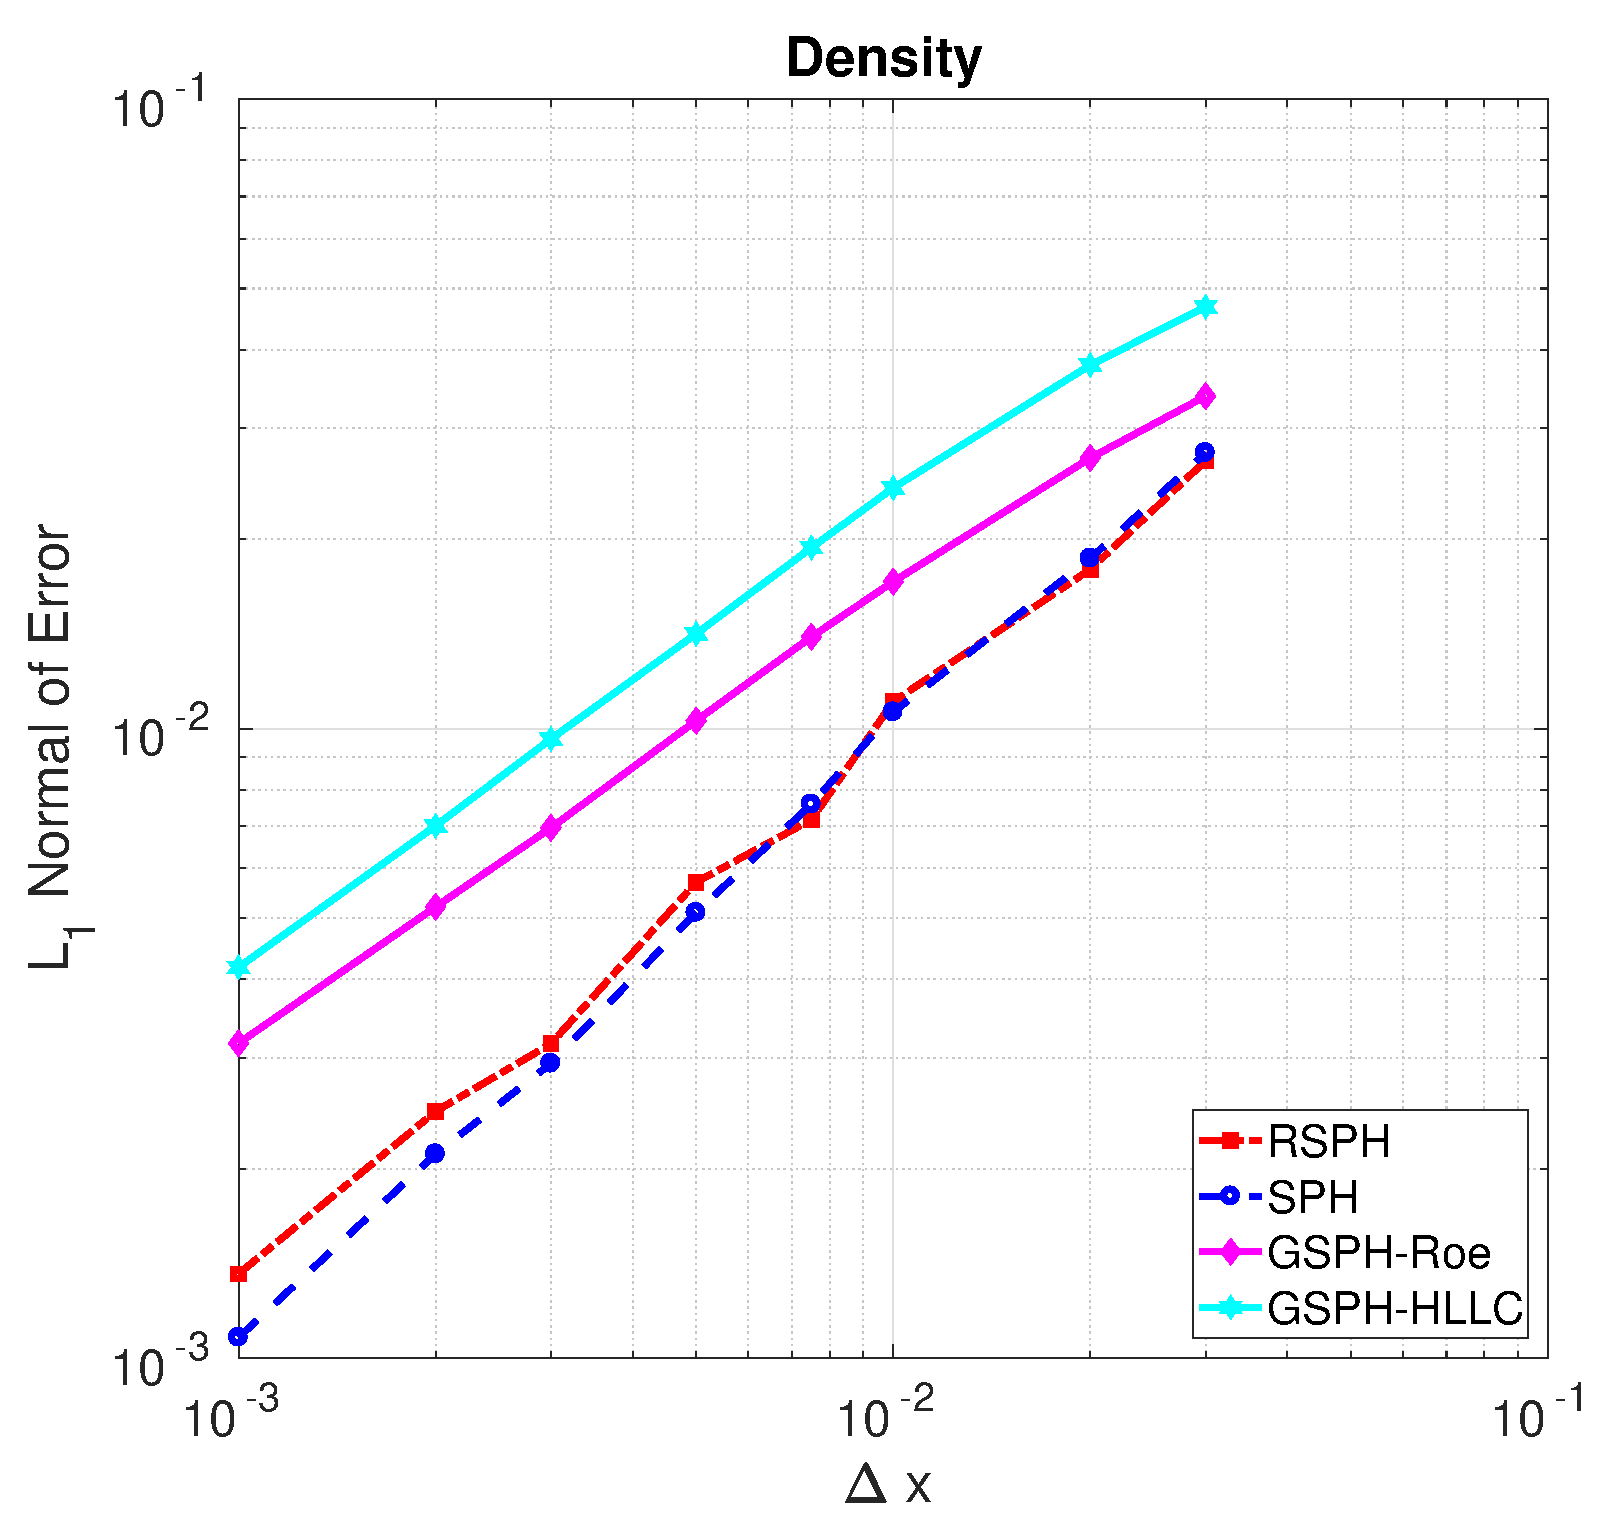
\includegraphics[width=0.99 \textwidth]{./Figures/Accuracy-des}
    \end{minipage}%
    \begin{minipage}{.332 \textwidth}
        \centering
        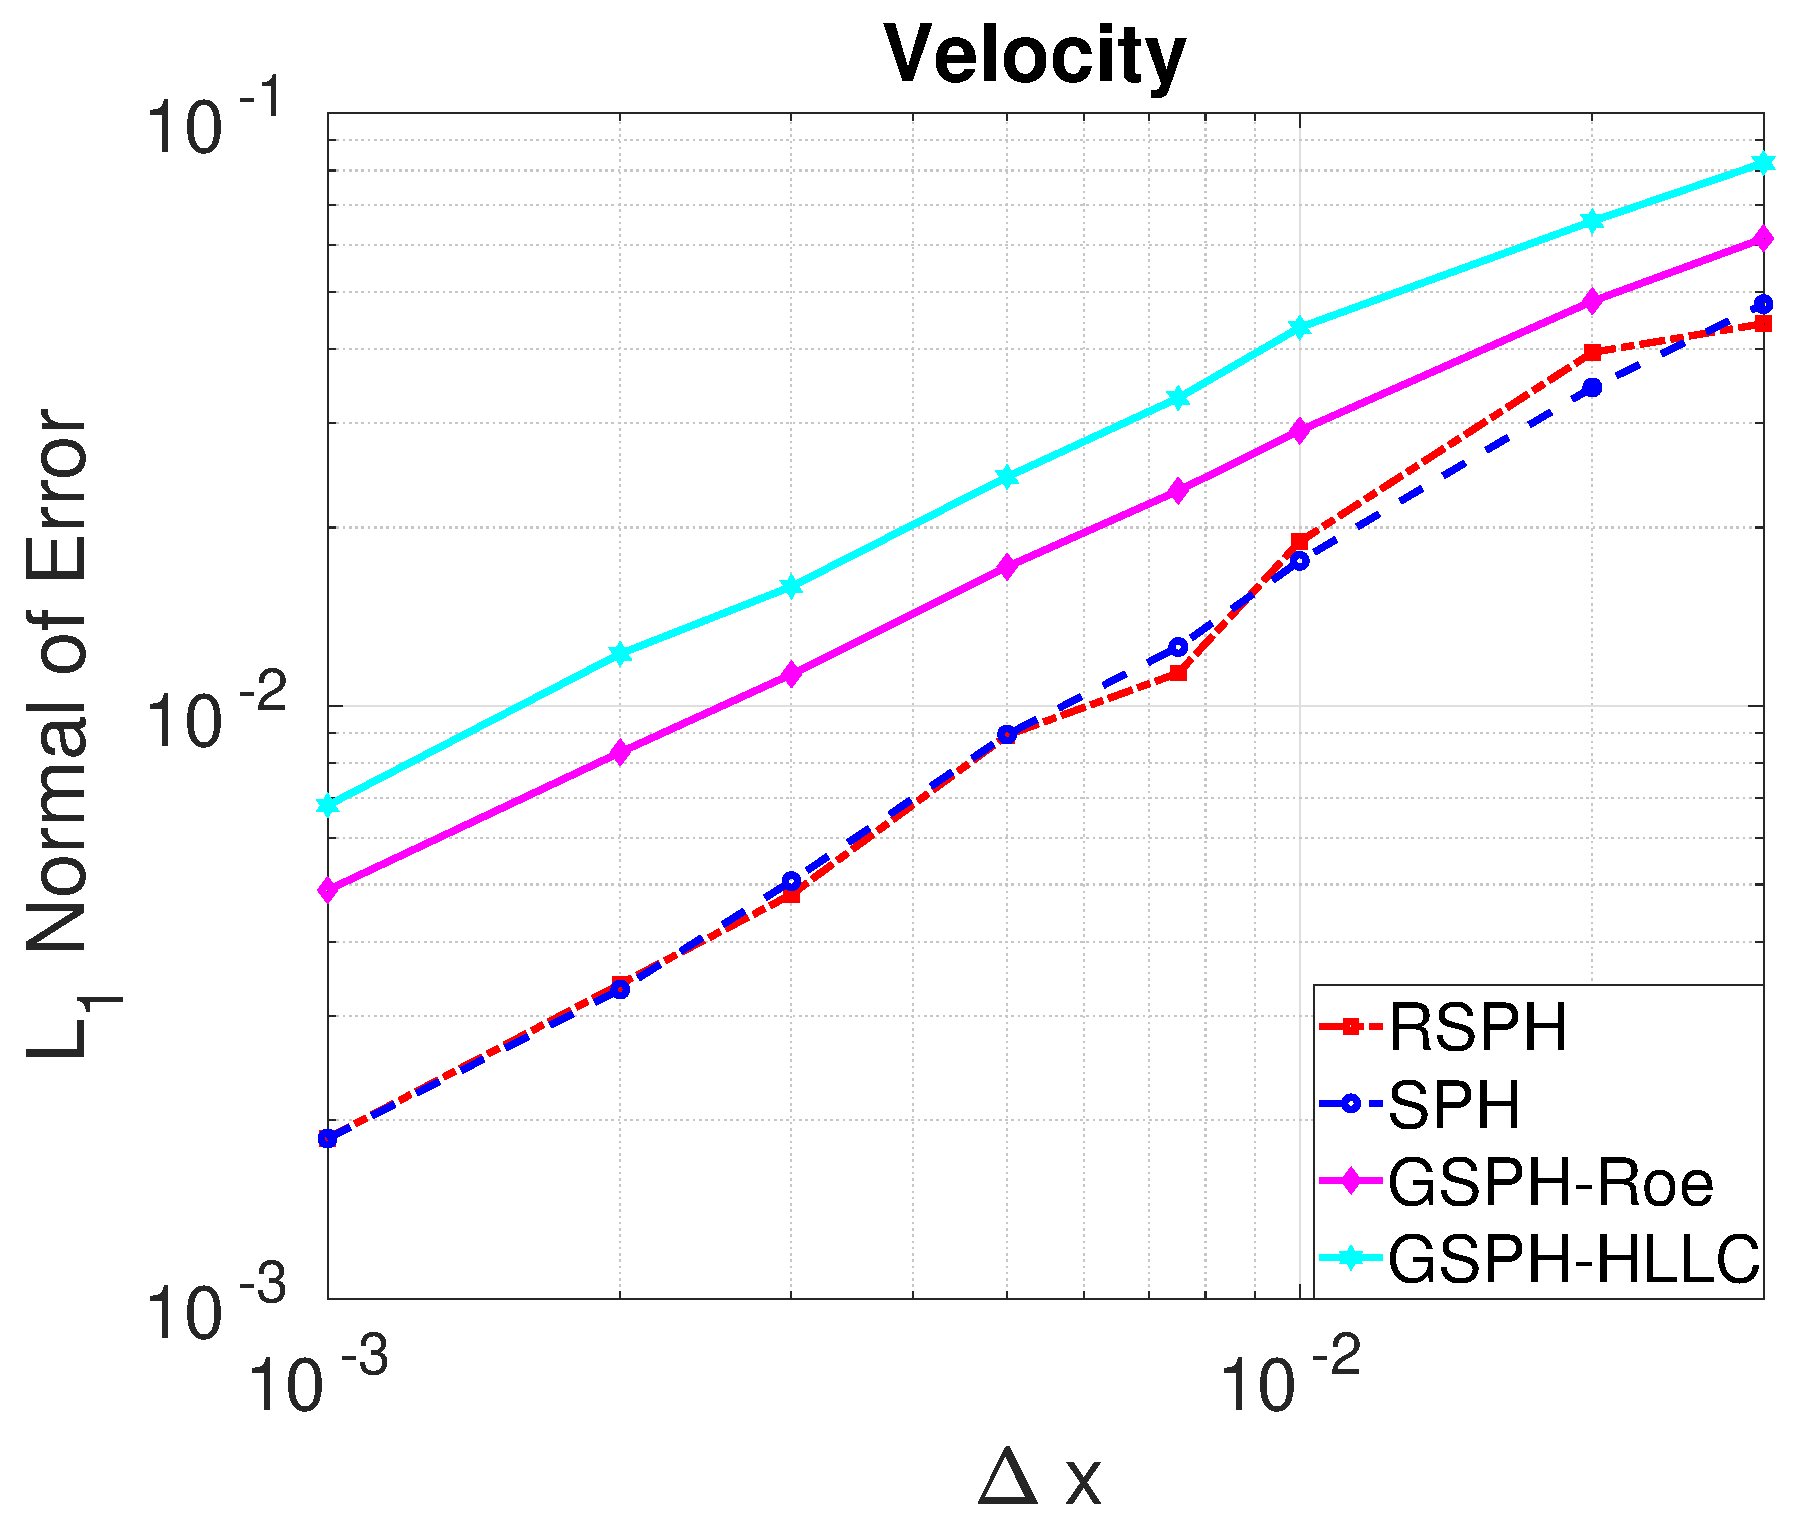
\includegraphics[width=0.99 \textwidth]{./Figures/Accuracy-vel}
    \end{minipage}%
    \begin{minipage}{.332\textwidth}
        \centering
        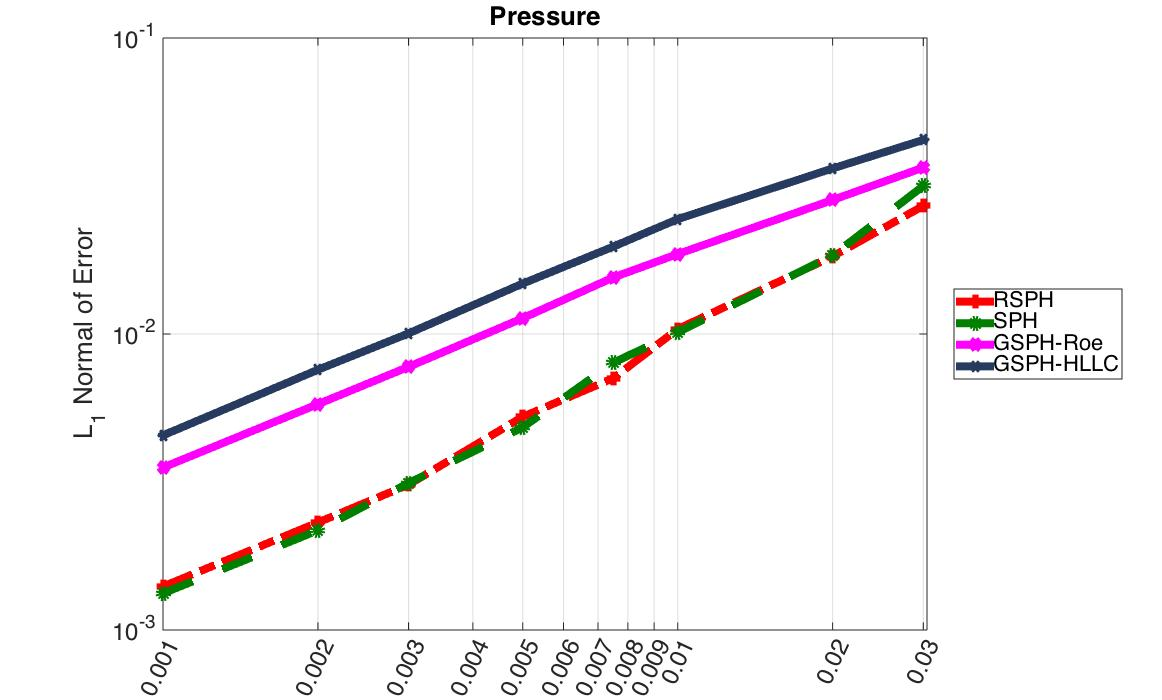
\includegraphics[width=0.99 \textwidth]{./Figures/Accuracy-pre}
    \end{minipage}%  
    \caption{ $L_1$ norm errors for 1D shock tube test (test1) for RSPH, standard SPH, GSPH using Roe Riemann solver and GSPH using HLLC Riemann Solver.  GSPH with the HLLC approximate Riemann solver exhibits the same convergence rate (around 1) but quantitatively larger errors than that with Roe Riemann solver. RSPH and standard SPH shows same rate of convergence and almost same amount of error.}
    \label{fig:Accuracy-test1}
\end{figure}
 
\subsection{Comprehensive 1D tests} \label{sec:comprehensive-1d-tests}
Comprehensive tests are presented in this section to check how well does RSPH work for different situations. Input parameters for each tests is given in Table \ref{tab:1D-shock-input_parameters}.
The results are shown in Fig. \ref{fig:RCM-GSPH-Sod} $\sim$ Fig. \ref{fig:RCM-strong-blast}. $x$ axis in these plots are normalized by the terminal time $t_f$. We observe that RSPH is able to correctly predict the position and magnitude of all waves for all tests. A jump of specific internal energy at the origin is observed in Sj$\ddot{o}$green test. However, such jump is a common issue of SPH schemes and has been reported in many other tests (see, for example, \citep{monaghan1997sph,cha2003implementations,puri2014approximate})
In addition, a noticeable spike can be observed near the contact discontinuity. Similar spike is observed in GSPH simulation \citep{puri2014comparison}. %Such spike is evident in the FVM solution as well and is perhaps an artifice of the Lagrangian nature of the two schemes. 
\citet{noh1987errors} proposed to adding a small amount of thermal conduction to ameliorate the spike and has been applied in blast-wave test using GSPH \citep{puri2014comparison}. We did not adopt such strategy in our simulation.
Due to less amount of dissipation, numerical fluctuations persist in all simulation results. For the strong blast test and double shock test, such fluctuations become more obvious than other tests, even though, the magnitude of fluctuations is within an acceptable range.

\begin{figure}[H]
    \centering
    \begin{minipage}{.415\textwidth}
        \centering
        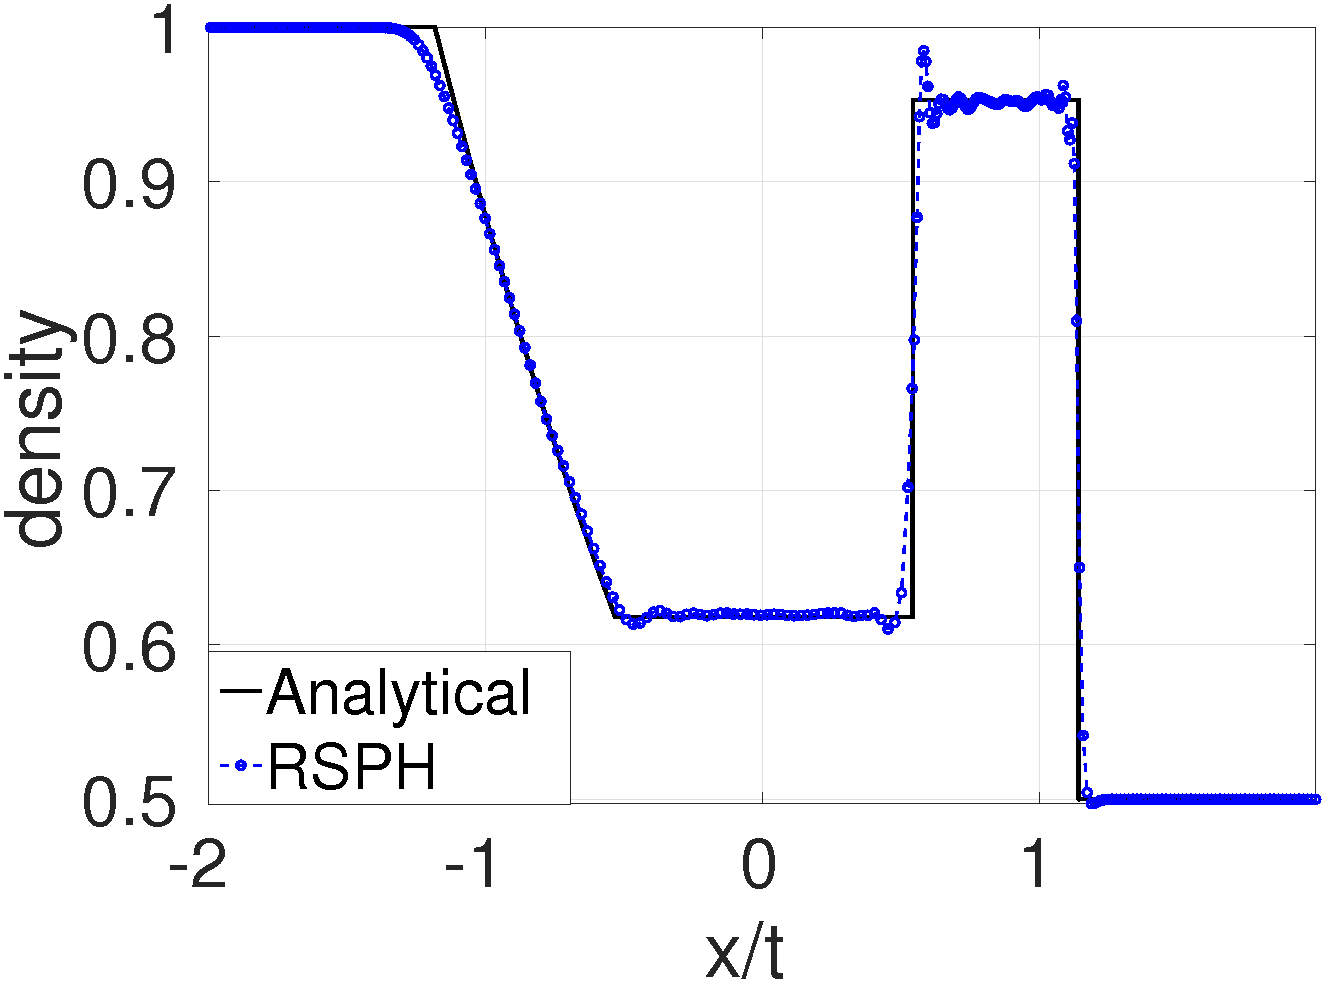
\includegraphics[width=0.99 \textwidth]{./Figures/GRod-RCM-rho}
    \end{minipage}%
    \begin{minipage}{.415 \textwidth}
        \centering
        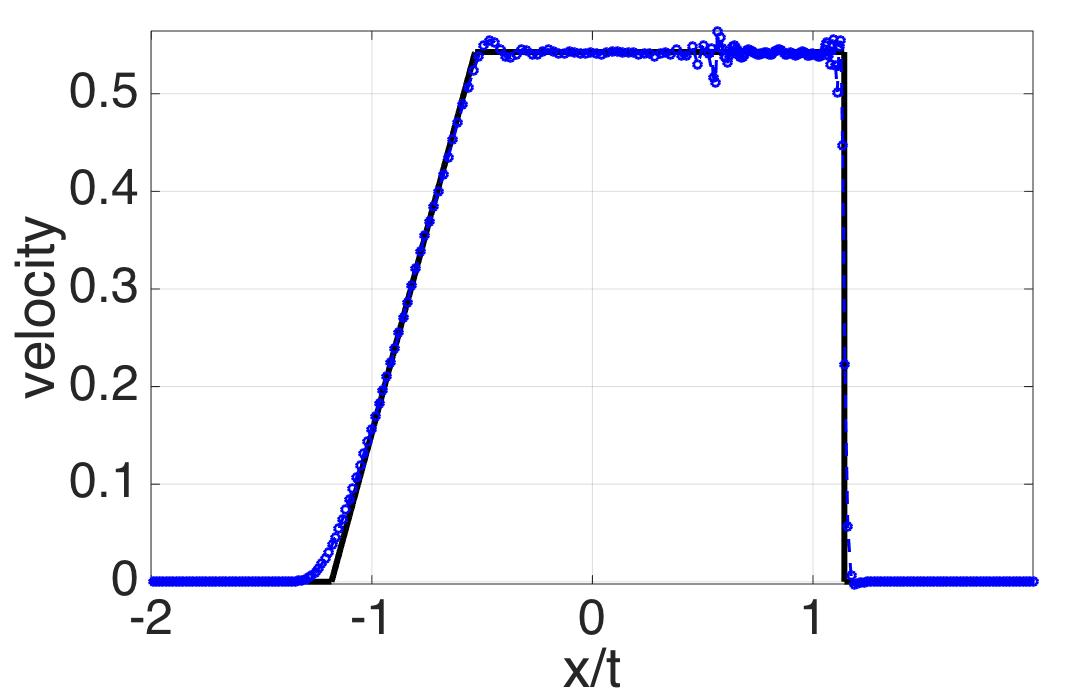
\includegraphics[width=0.99 \textwidth]{./Figures/GRod-RCM-v}
    \end{minipage}% 
    \\
    \begin{minipage}{.415\textwidth}
        \centering
        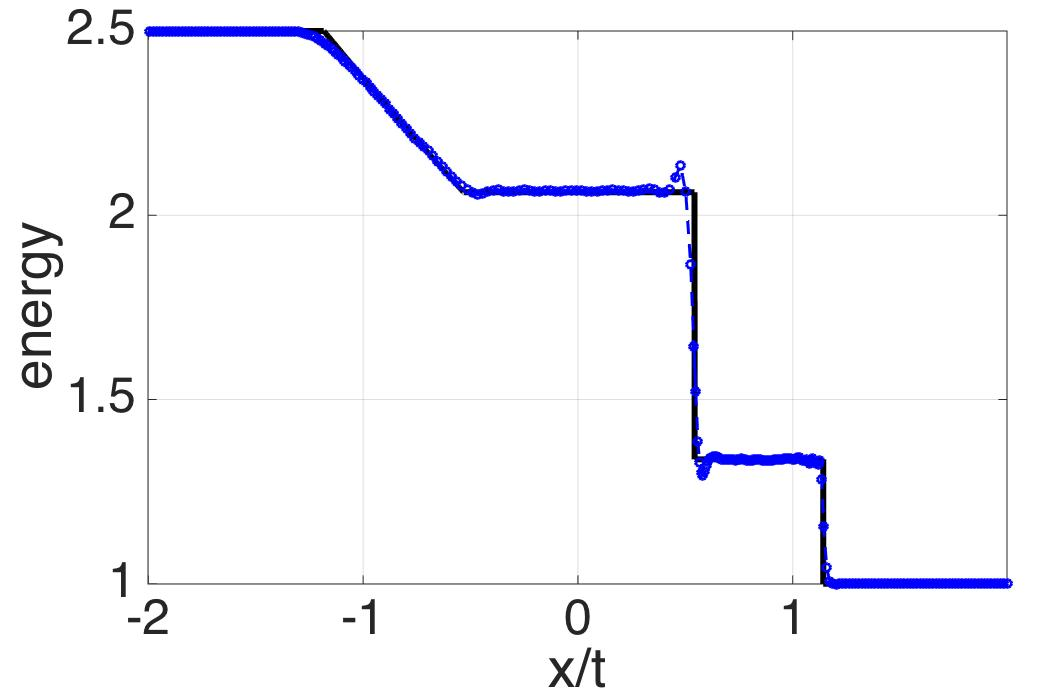
\includegraphics[width=0.99 \textwidth]{./Figures/GRod-RCM-e}
    \end{minipage}%
    \begin{minipage}{.415 \textwidth}
        \centering
        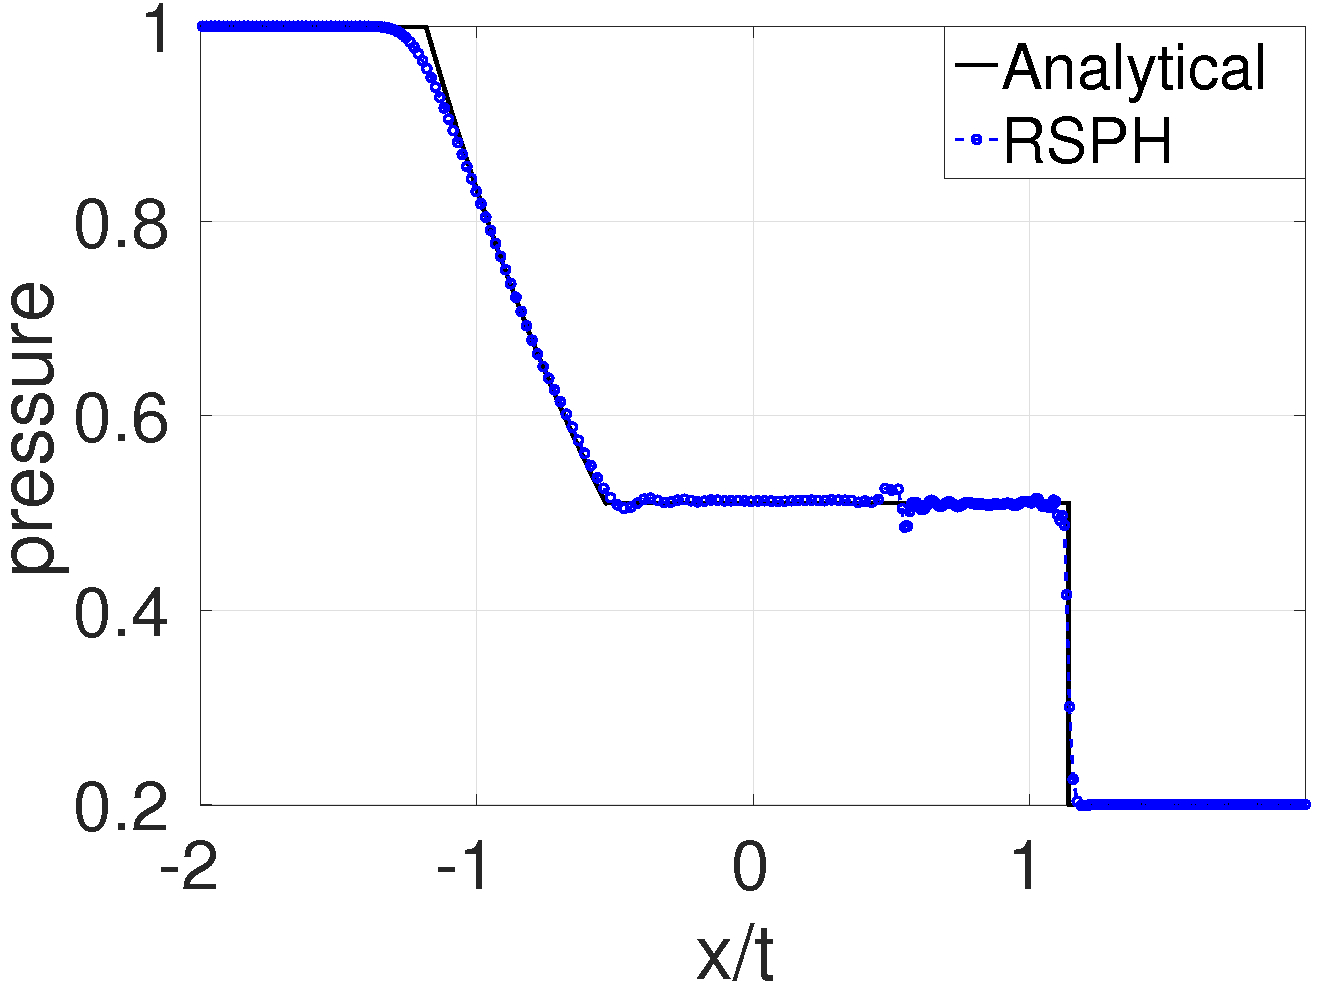
\includegraphics[width=0.99 \textwidth]{./Figures/GRod-RCM-p}
    \end{minipage}% 
    \caption{Results for test 2, a variation of Sod test. All physical properties are well re-produced except for some acceptable oscillations}
    \label{fig:RCM-GSPH-Sod}
\end{figure}

\begin{figure}[H]
    \centering
    \begin{minipage}{.415\textwidth}
        \centering
        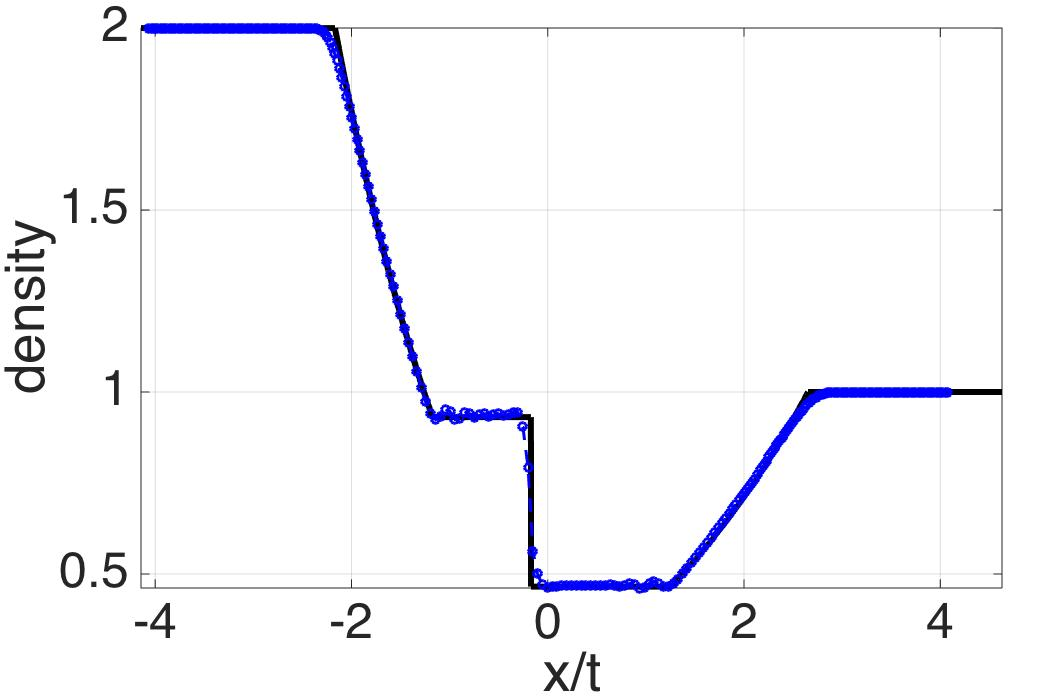
\includegraphics[width=0.99 \textwidth]{./Figures/Dexp-RCM-rho}
    \end{minipage}%
    \begin{minipage}{.415 \textwidth}
        \centering
        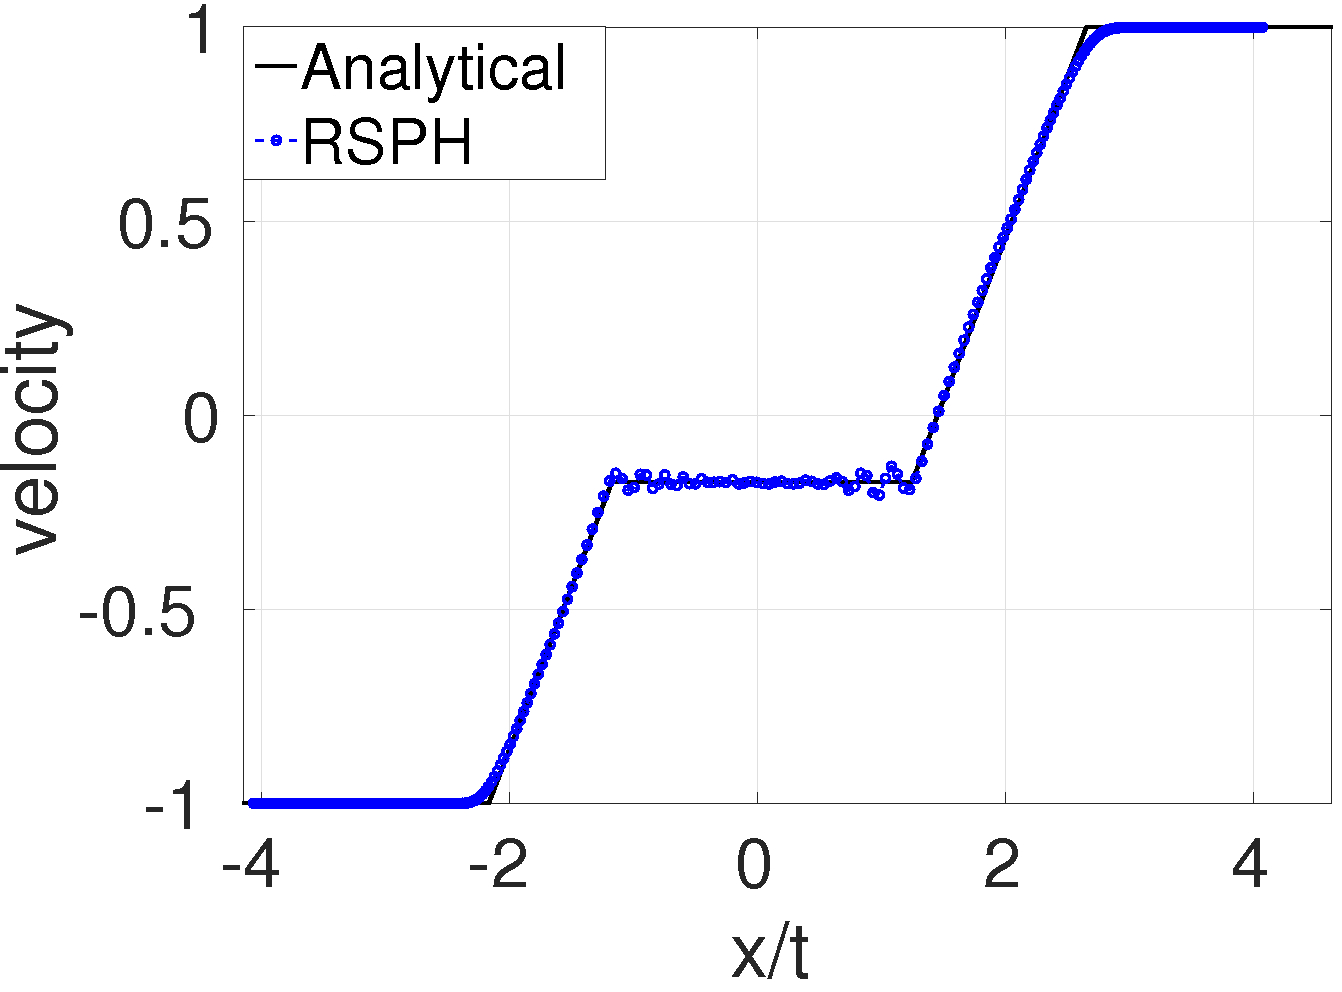
\includegraphics[width=0.99 \textwidth]{./Figures/Dexp-RCM-v}
    \end{minipage}%
    \\
    \begin{minipage}{.415\textwidth}
        \centering
        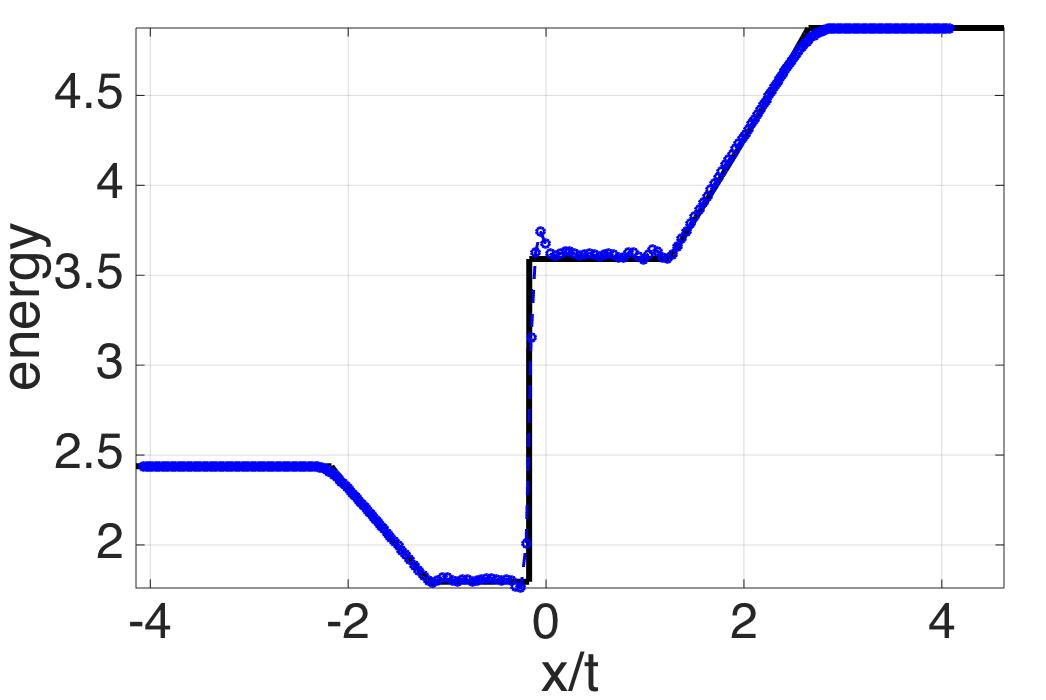
\includegraphics[width=0.99 \textwidth]{./Figures/Dexp-RCM-e}
    \end{minipage}%
    \begin{minipage}{.415 \textwidth}
        \centering
        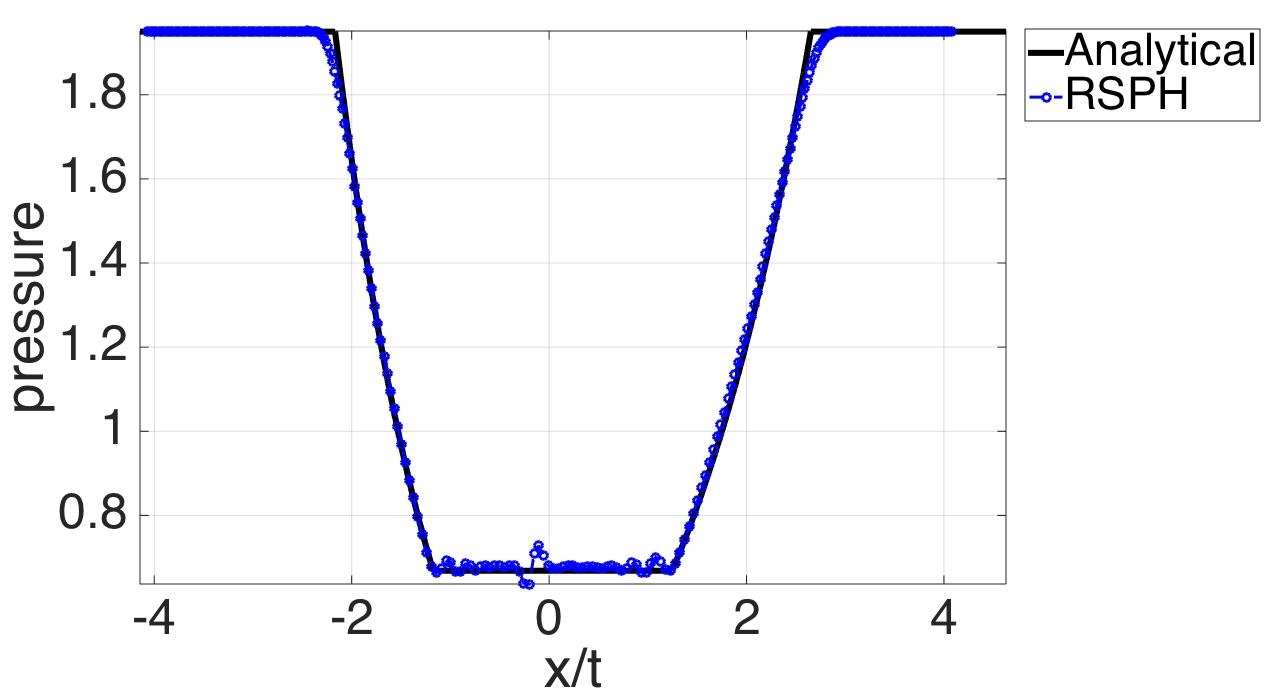
\includegraphics[width=0.99 \textwidth]{./Figures/Dexp-RCM-p}
    \end{minipage}% 
    \caption{Results for test 3, the double expansion case. All physical properties are well re-produced except for some oscillations}
    \label{fig:RCM-double-expansion}
\end{figure}

\begin{figure}[H]
    %\centering
    \begin{minipage}{.415\textwidth}
        \centering
        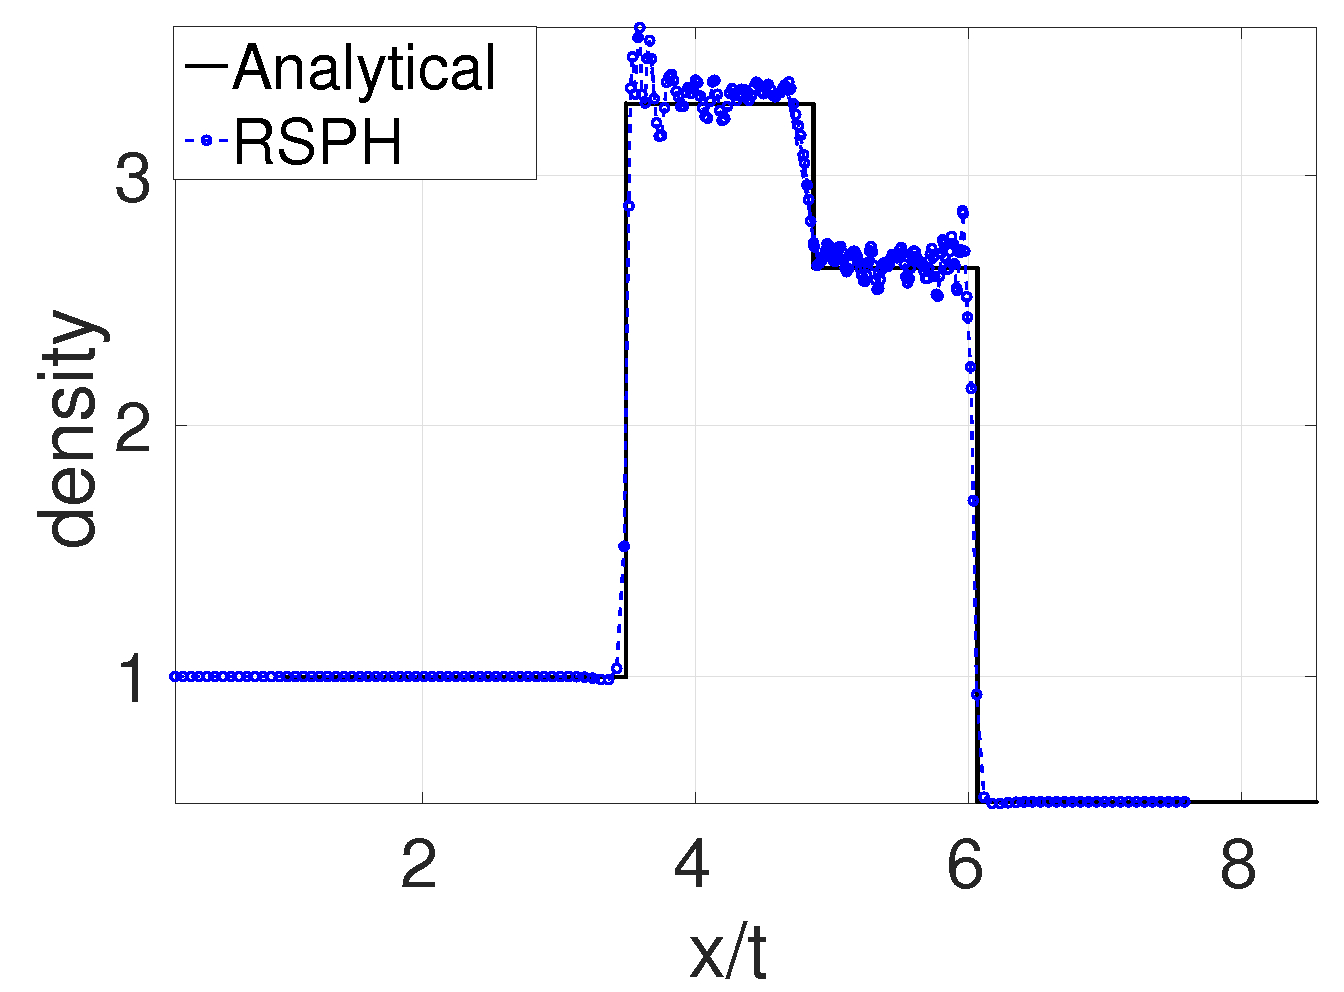
\includegraphics[width=0.99 \textwidth]{./Figures/Dshock-RCM-rho-Rp6}
    \end{minipage}%
    \begin{minipage}{.415 \textwidth}
        \centering
        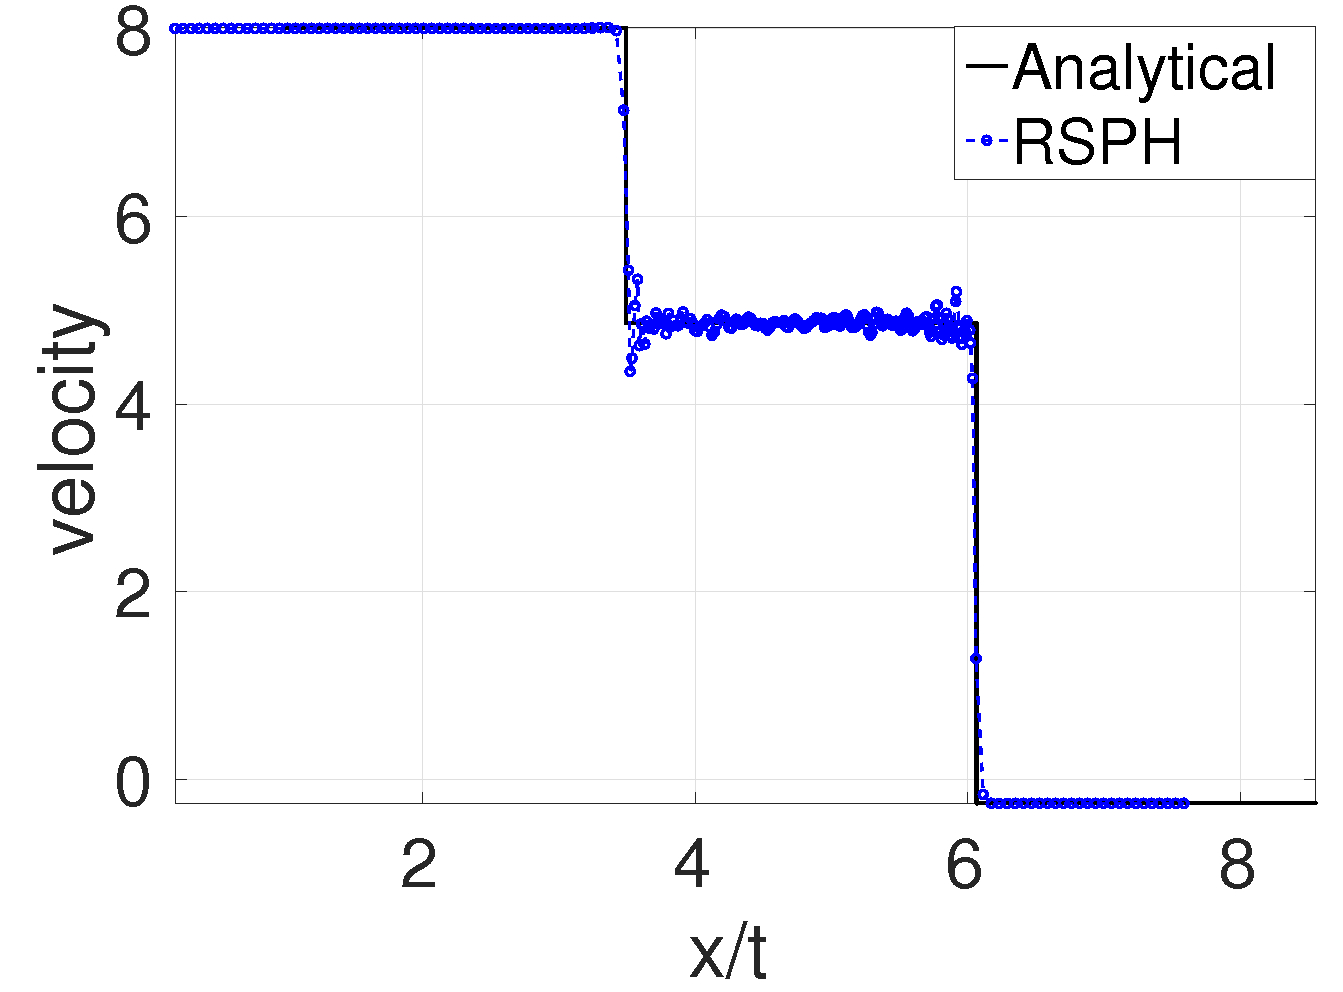
\includegraphics[width=0.99 \textwidth]{./Figures/Dshock-RCM-v-Rp6}
    \end{minipage}%
    \\
    \begin{minipage}{.415\textwidth}
        \centering
        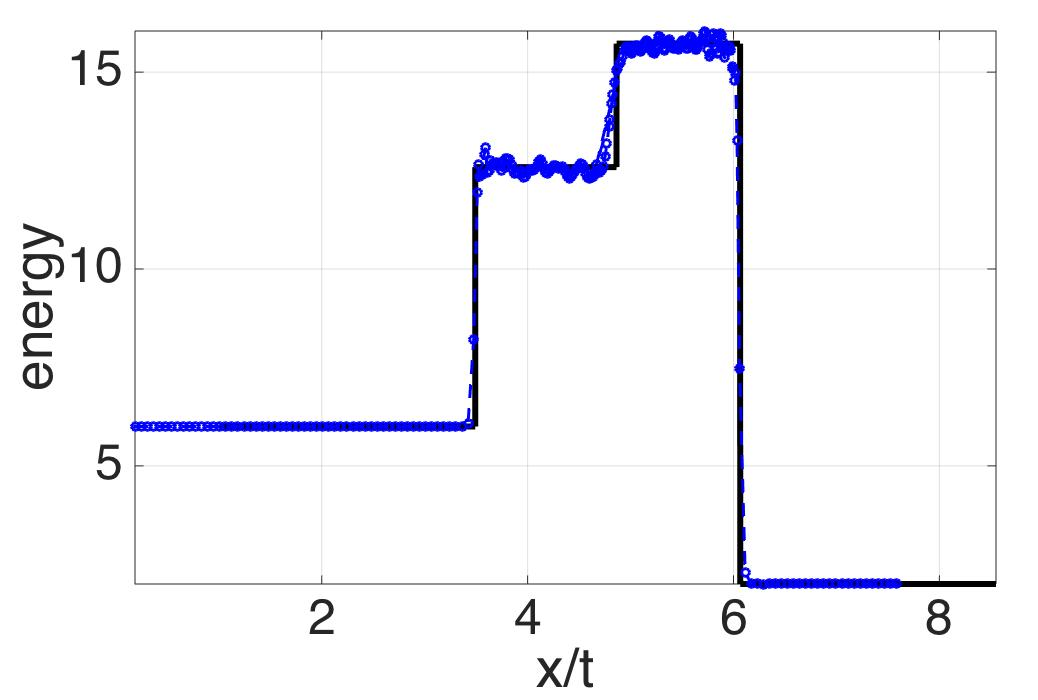
\includegraphics[width=0.99 \textwidth]{./Figures/Dshock-RCM-e-Rp6}
    \end{minipage}%
    \begin{minipage}{.415 \textwidth}
        \centering
        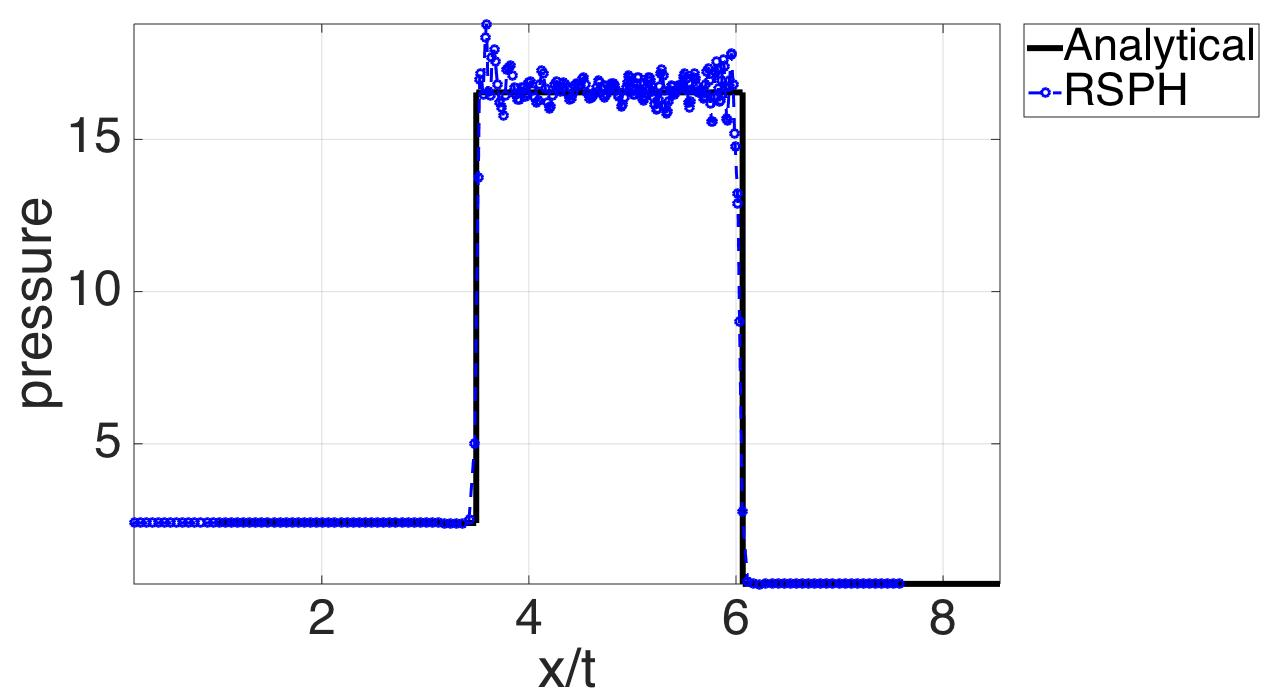
\includegraphics[width=0.99 \textwidth]{./Figures/Dshock-RCM-p-Rp6}
    \end{minipage}% 
    \caption{Results for test 4, the double shock case. To stabilize the simulation, RSPH sampling is in a narrower range. All physical properties are well re-produced. However, the oscillations are more serious than oscillations in other tests.}
    \label{fig:RCM-double-shock}
\end{figure}

\begin{figure}[H]
    \begin{minipage}{.415\textwidth}
        \centering
        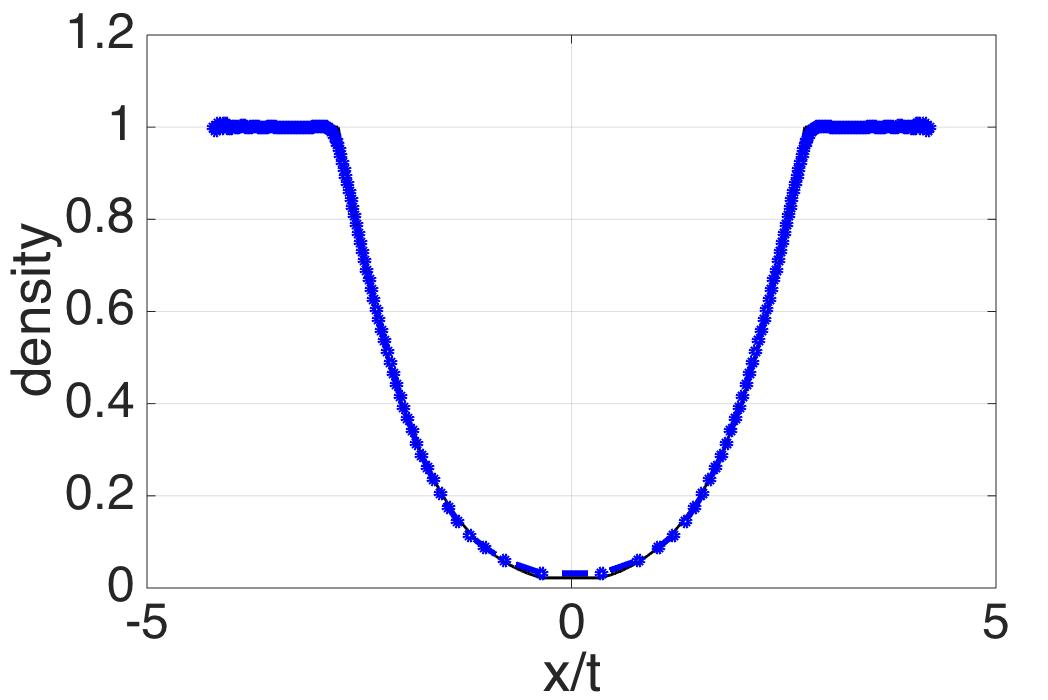
\includegraphics[width=0.99 \textwidth]{./Figures/Sjogreen-RCM-rho-Adpt1}
    \end{minipage}%
    \begin{minipage}{.415 \textwidth}
        \centering
        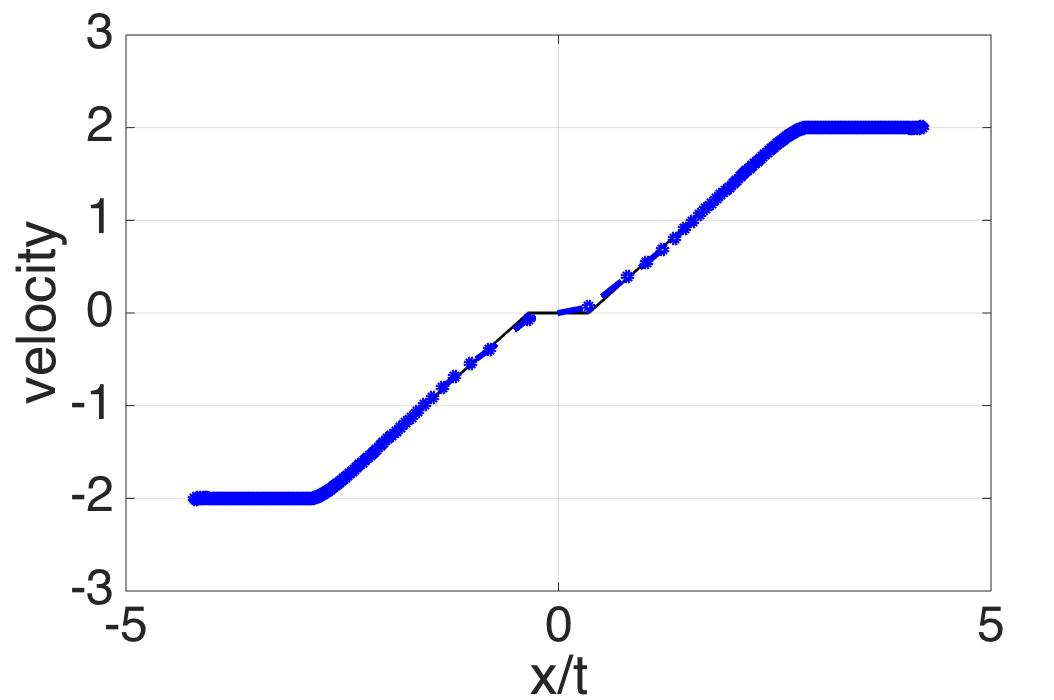
\includegraphics[width=0.99 \textwidth]{./Figures/Sjogreen-RCM-v-Adpt1}
    \end{minipage}%
    \\
    \begin{minipage}{.415\textwidth}
        \centering
        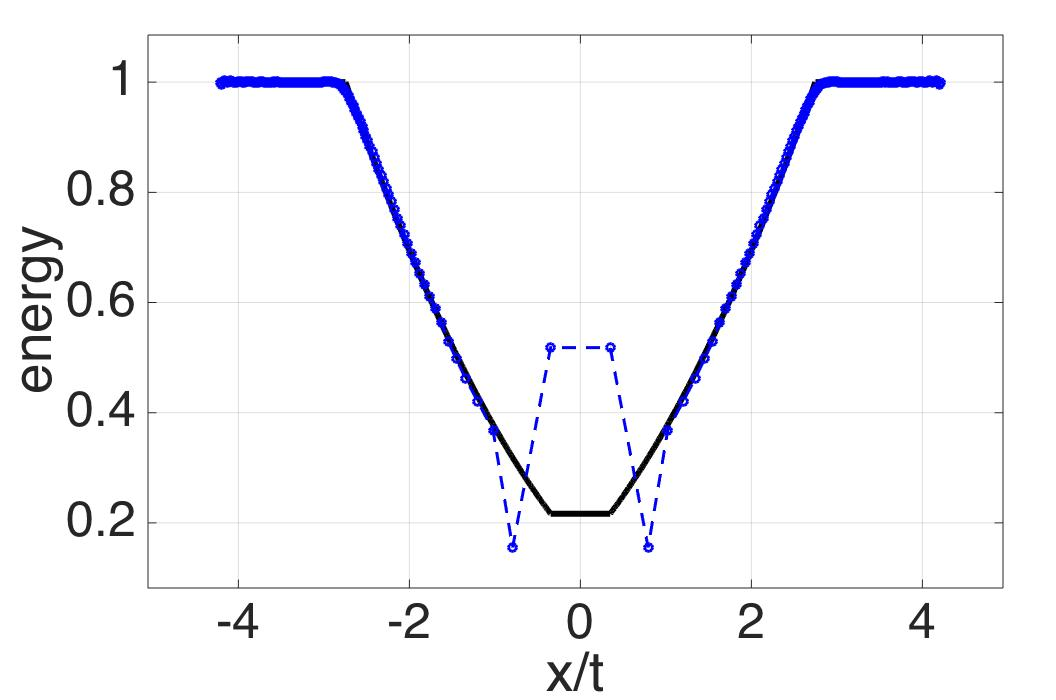
\includegraphics[width=0.99 \textwidth]{./Figures/Sjogreen-RCM-e-Adpt1}
    \end{minipage}%
    \begin{minipage}{.415 \textwidth}
        \centering
        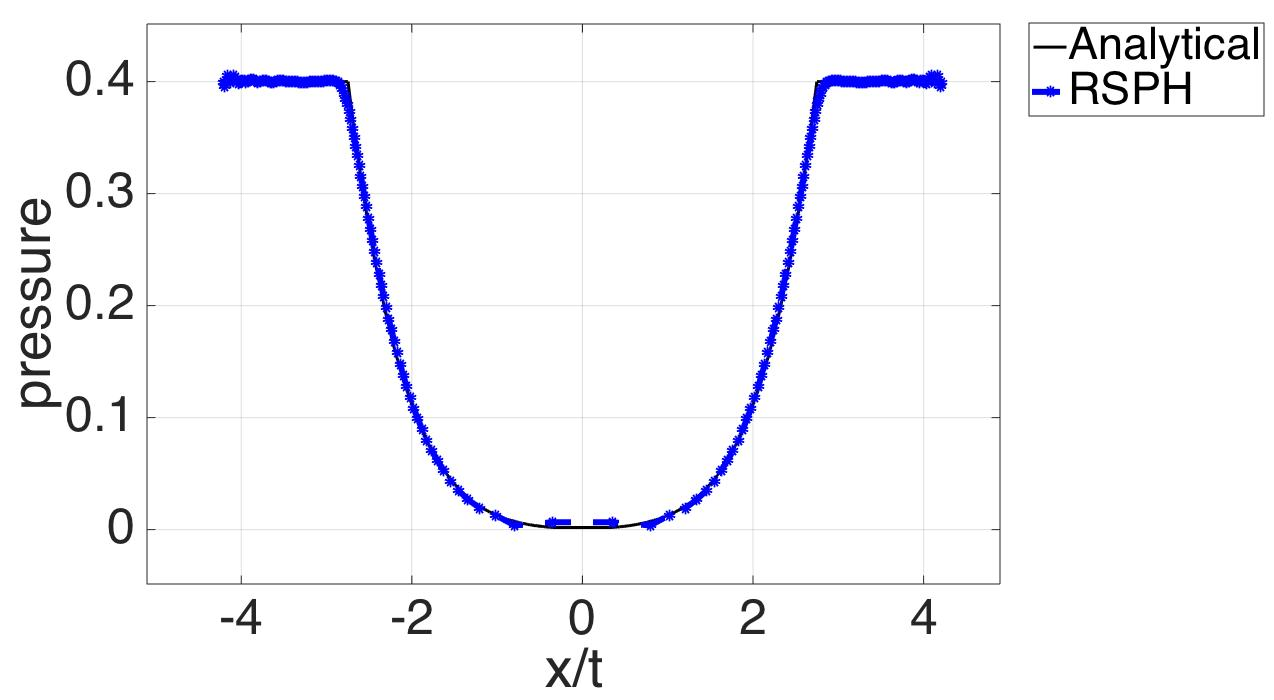
\includegraphics[width=0.99 \textwidth]{./Figures/Sjogreen-RCM-p-Adpt1}
    \end{minipage}% 
    \caption{Results for test 5, a variation of the Sj$\ddot{o}$green test. The density, velocity and pressure are well re-produced while the thermal energy at the origin is poorly predicted. A jump of internal energy at the origin is a common issue in many SPH schemes (see, for example, \citep{monaghan1997sph,cha2003implementations,puri2014approximate})}
    \label{fig:RCM-Sjogreen}
\end{figure}

\begin{figure}[H]
    \centering
    \begin{minipage}{.415\textwidth}
        \centering
        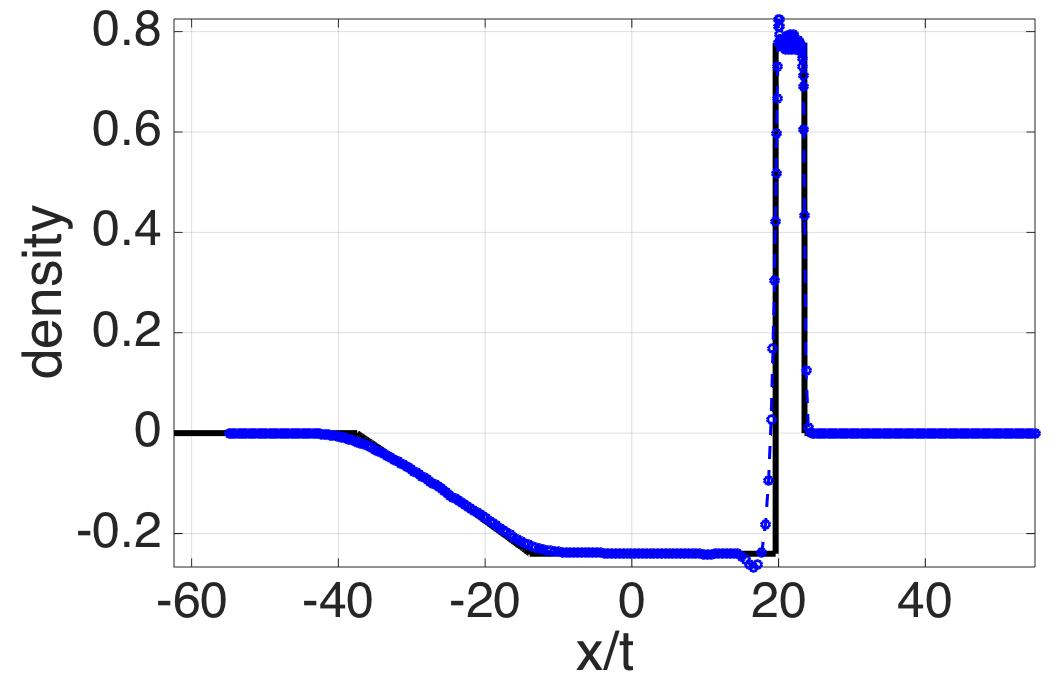
\includegraphics[width=0.99 \textwidth]{./Figures/StrBlst-RCM-rho-Rp3}
    \end{minipage}%
    \begin{minipage}{.415 \textwidth}
        \centering
        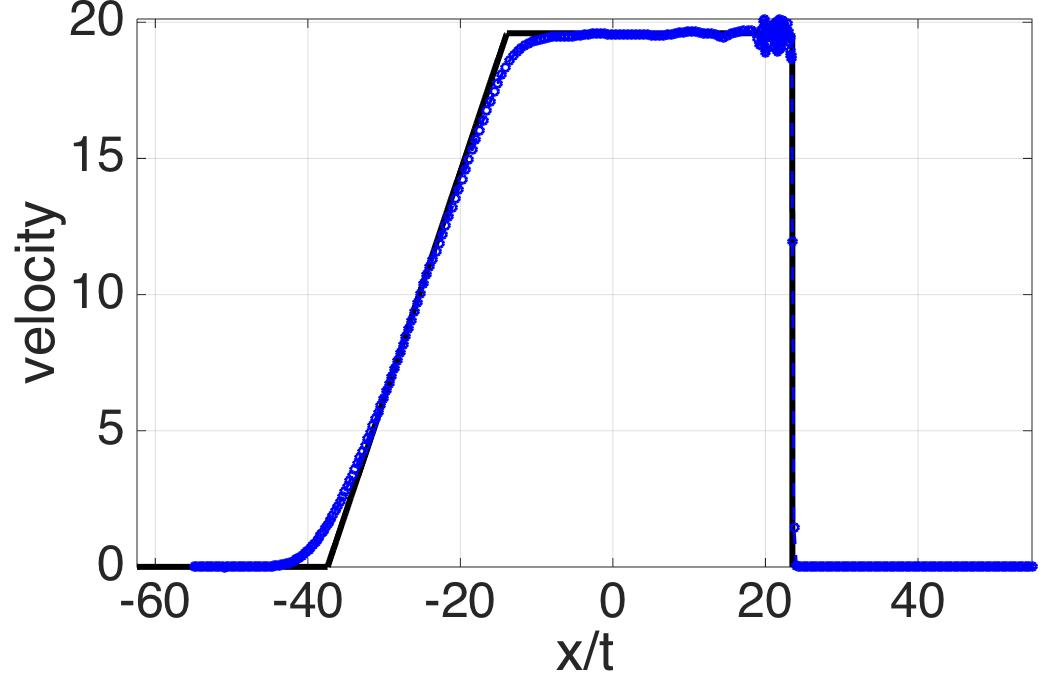
\includegraphics[width=0.99 \textwidth]{./Figures/StrBlst-RCM-v-Rp3}
    \end{minipage}%
    \\
    \begin{minipage}{.415 \textwidth}
        \centering
        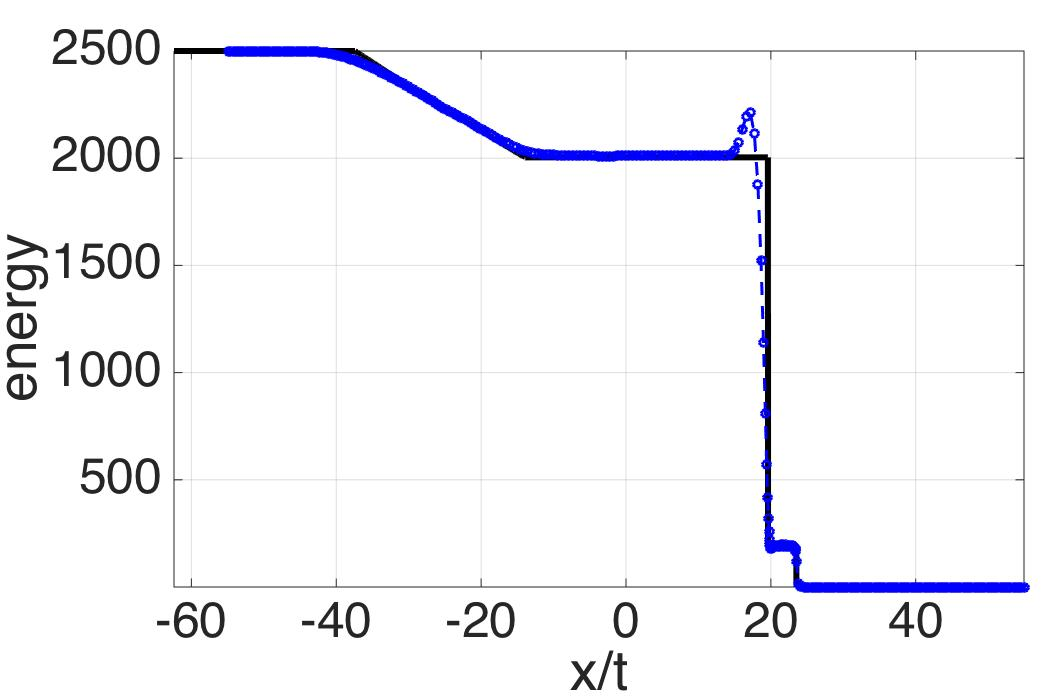
\includegraphics[width=0.99 \textwidth]{./Figures/StrBlst-RCM-e-Rp3}
    \end{minipage}%
    \begin{minipage}{.415 \textwidth}
        \centering
        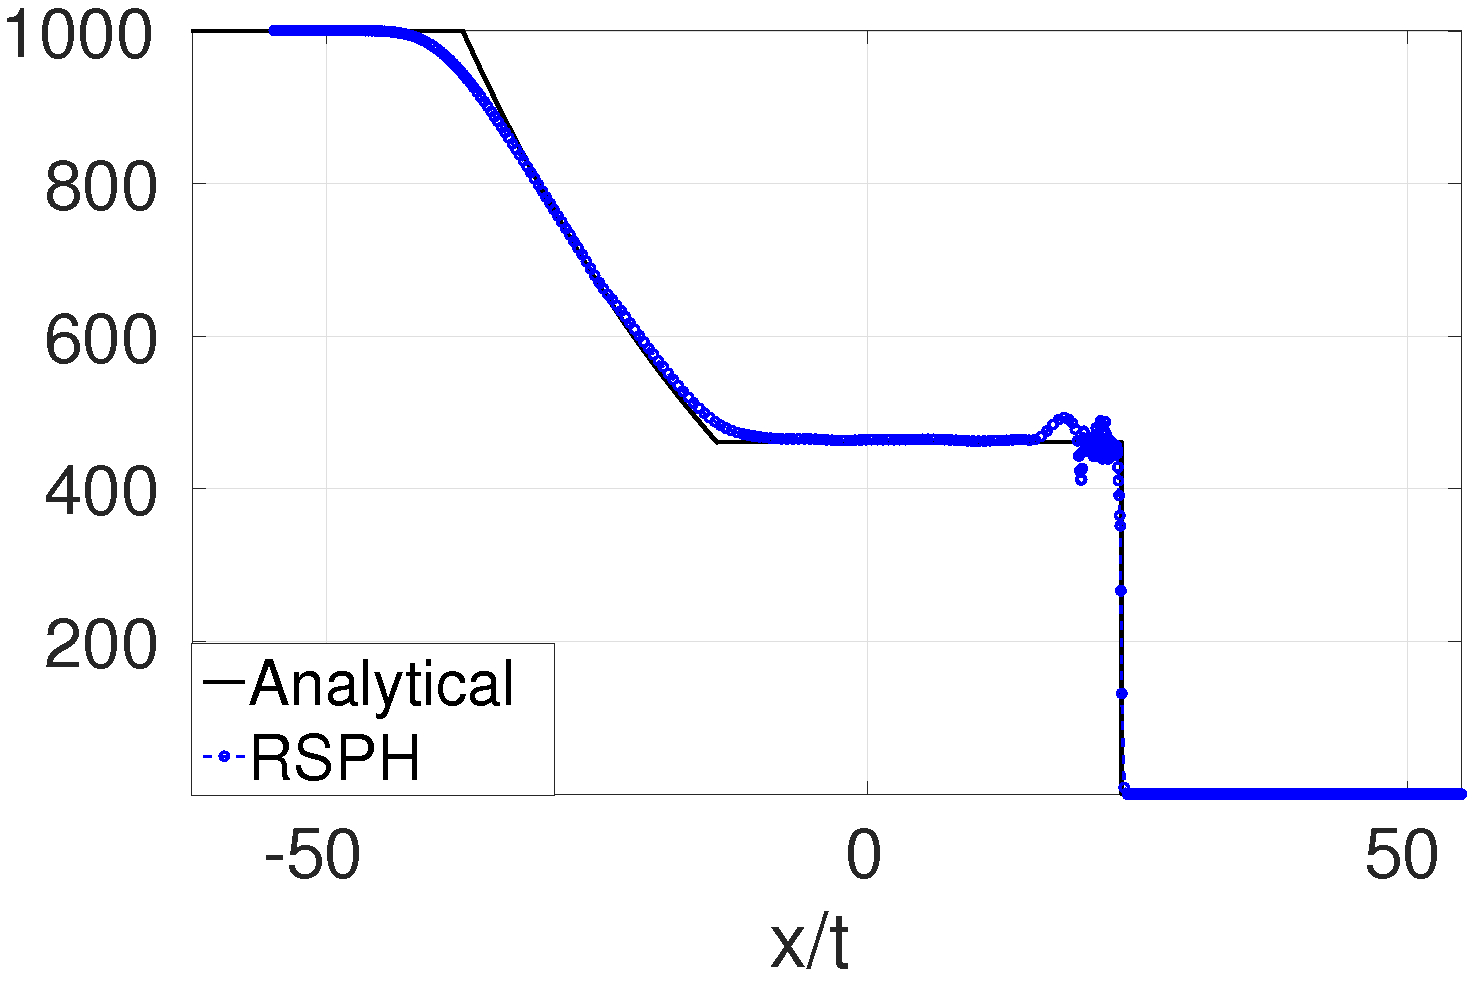
\includegraphics[width=0.99 \textwidth]{./Figures/StrBlst-RCM-p-Rp3}
    \end{minipage}% 
    \caption{Results for test 6, the strong blast test. y axis for density plot is in log base 10.  To stabilize the simulation, RSPH sampling is in a narrower range. All physical properties are well re-produced. The oscillations between shock and contact discontinuity is relatively larger than other area. A noticeable spike is observed near contact discontinuity.}
    \label{fig:RCM-strong-blast}
\end{figure}

\subsection{3D free jet} \label{jet}
Free jet flow have been studied analytically, experimentally and numerically for many decades, not only because of its wide application but also because of its fundamental significance as a basic flow to the scientific research community. To test the capacity of RSPH for multiple dimensional applications, a free jet flow is simulated in this section by solving 3D compressible Euler Equations using standard SPH, GSPH and RSPH. 
All simulations are using the same set-up and compared at the same physical time. In this test, RSPH simulation is carried out based on piece wise constant construction of Riemann problem and a HLLC approximate Riemann solver. To do a well-controlled comparison, GSPH adopts the same way for Riemann problem construction and the same Riemann solver as RSPH. 

The computational domain in this test is a box. The boundaries can be categorized into the velocity inlet (a circular area at the center of the bottom of the box), non-slip wall boundary (box bottom) and pressure outlet (other faces of the box). The boundaries are set away from vent to avoid boundary effects on simulation.
At the vent, exit velocity $\textbf{v}$ is set to $500 m / s$ and radius of the nozzle $r$ is set to $8m $. The pressure of ejected fluid is assumed to be the same as ambient ($101 kpa$). The temperature of both ejected fluids and ambient fluids are set to $273 K$. 
Velocity is zero for non-slip wall boundary. The heat flux across wall boundary is zero assuming an adiabatic wall. The flux of mass should also be zero on the wall. As a result, internal energy flux, which consists of heat flux and energy flux carried by mass flux, vanishes on the wall boundary. 
The pressure of the surrounding ambient is given. As we ignore the physical viscosity, the shear stress is ignored and normal stress (whose magnitude equals to pressure) balances the ambient pressure.
\begin{equation}
p = p_a\left(z\right)  \label{eq:pressure_bc_p} 
\end{equation} 
Except for the pressure, boundary values for density, velocity, and energy on the outlet are dependent on solution. Fluids properties of ideal gas are used in this simulation.

\begin{figure}[H]
    \centering
    \begin{minipage}[t]{.325\textwidth}
        \centering
        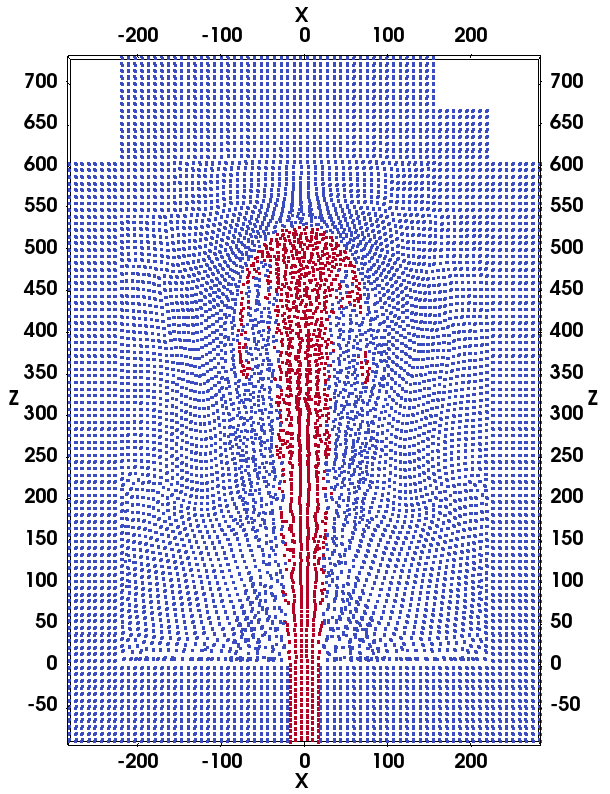
\includegraphics[width=0.99 \textwidth]{./Figures/SPH-alf2-t3-cutView}
    \end{minipage}%
    \begin{minipage}[t]{.325 \textwidth}
        \centering
        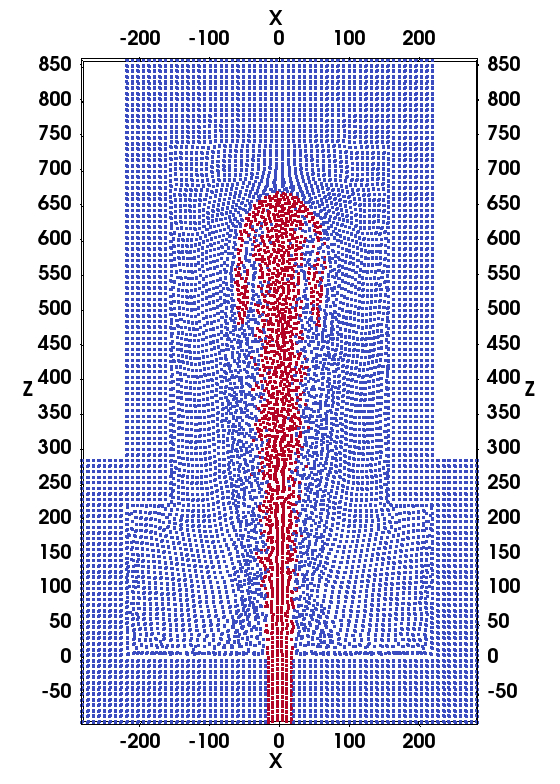
\includegraphics[width=0.99 \textwidth]{./Figures/SPH-alf1-t3-cutView}
    \end{minipage}%
    \begin{minipage}[t]{.325\textwidth}
        \centering
        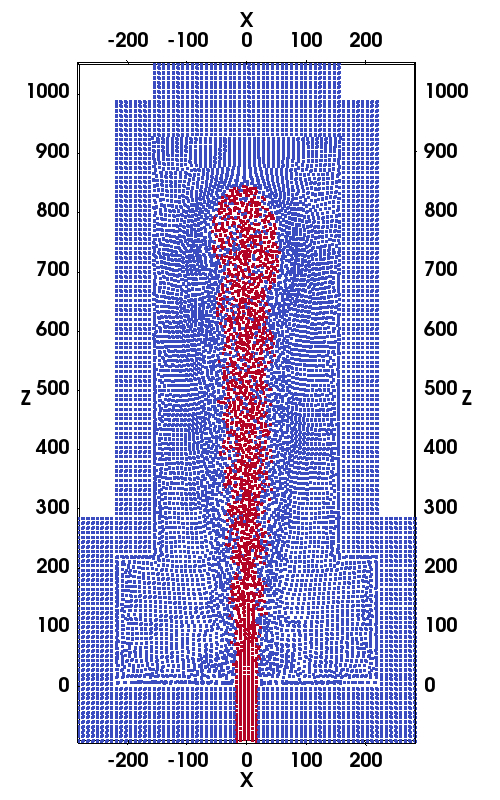
\includegraphics[width=0.99 \textwidth]{./Figures/SPH-alfp3-t3-cutView}
    \end{minipage}%
    \caption{Free jet flow simulation results at $t=3.0 s$ by SPH using different artificial viscosity coefficients. These pictures are front view of a slice of the domain cut by two planes parallel to $x-z$ plane at $y=-9$ and $y=9$. From left to right, the picture is corresponding to $\alpha=0.3$, $\alpha=1.0$ and $\alpha=2.0$ respectively. Another artificial viscosity coefficient $\beta$ is set to be double of $\alpha$ for all tests. Red particles in pictures are particles erupted from the nozzle while blues are ambient fluids particles.}
    \label{fig:free-jet-SPH-comparison}
\end{figure}

\begin{figure}[H]
    \centering
    \begin{minipage}[t]{.325 \textwidth}
        \centering
        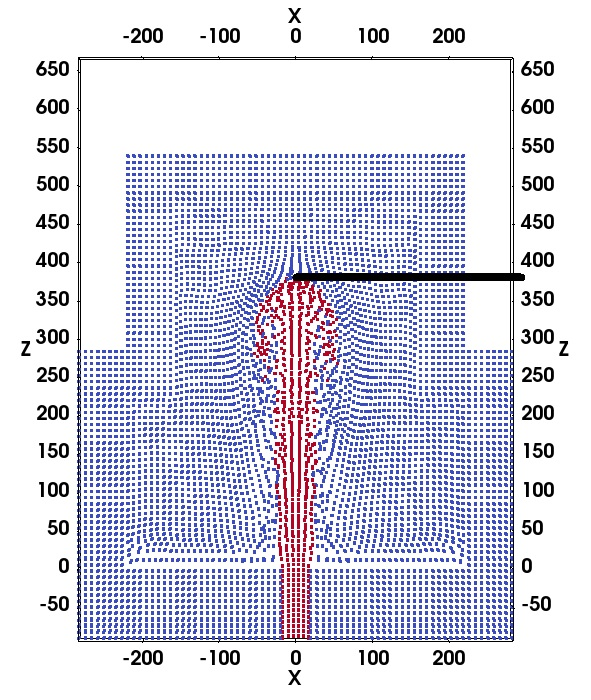
\includegraphics[width=0.99 \textwidth]{./Figures/GSPH-HLLC-t1p5-cutView}
    \end{minipage}%
    \begin{minipage}[t]{.325\textwidth}
        \centering
        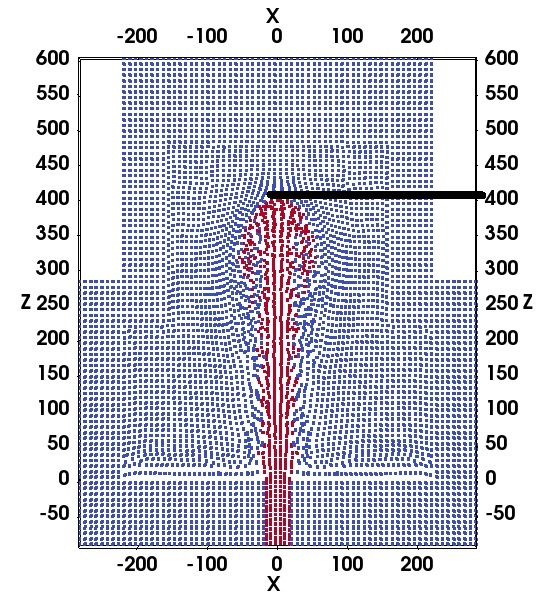
\includegraphics[width=0.99 \textwidth]{./Figures/RSPH-t1p5-cutView}
    \end{minipage}%
    \\
    \centering
    \begin{minipage}[t]{.325 \textwidth}
        \centering
        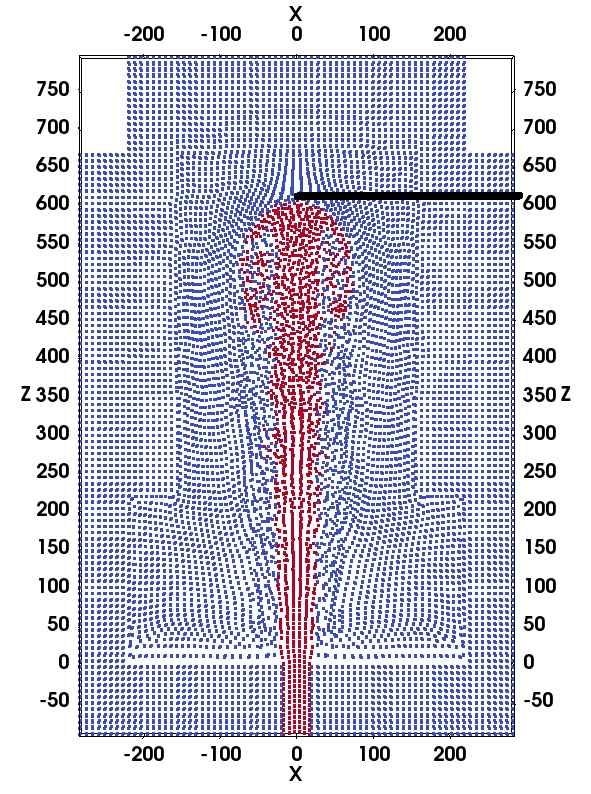
\includegraphics[width=0.99 \textwidth]{./Figures/GSPH-HLLC-t3-cutView}
    \end{minipage}%
    \begin{minipage}[t]{.325\textwidth}
        \centering
        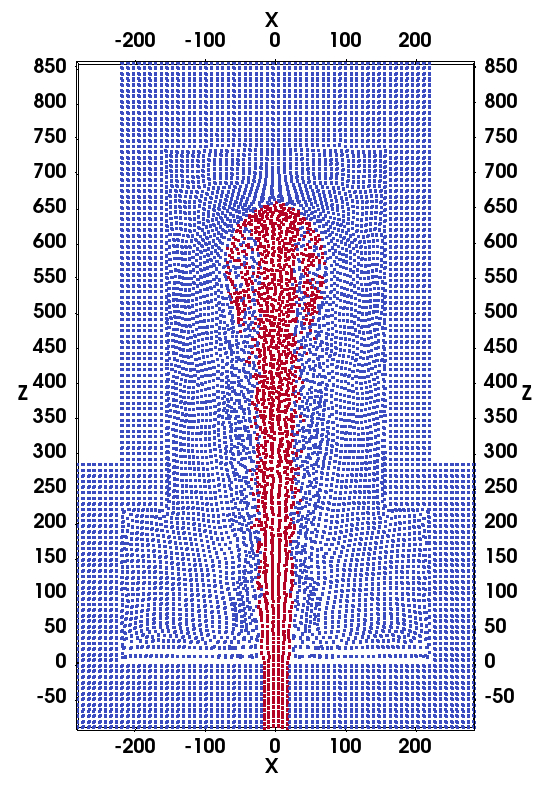
\includegraphics[width=0.99 \textwidth]{./Figures/RSPH-t3-cutView}
    \end{minipage}%
    \caption{Simulation results of free jet flow by SPH with $\alpha=1.0, \beta=2.0$, GSPH and RSPH. These pictures are front view of a slice of the domain cut by two planes parallel to $x-z$ plane at $y=-9$ and $y=9$. From left to right, the picture is corresponding to SPH, GSPH and RSPH respectively. Red particles in pictures are particles erupted from the nozzle while blues are ambient fluids particles. Pictures on the first row are corresponding to $t=1.5s$ while pictures on the second row are for $t=3.0 s$}
    \label{fig:free-jet-comparison}
\end{figure}

Figure \ref{fig:free-jet-SPH-comparison} shows simulation results of the free jet flow by SPH with different artificial viscosity coefficients. The overall damping effect due to artificial dissipation is clearly shown in this figure. We observe that the lengths to which these jets reach at $t=3.0 s$ are different when using different artificial viscosity coefficient. It is obvious that the larger artificial viscosity, the shorter length the jet can reach. The length that free jet reaches can be used as an indicator of overall dissipation. While introducing undesirable damping effects, artificial viscosity is necessary for numerical stability and simulating of shocks. So, in real applications, the artificial viscosity coefficients are usually tuned (see, for example, \citep{gmd-2017-119}) to minimize artificial damping effects.

We compare RSPH with GSPH in terms of equivalent overall artificial damping effects in Fig. \ref{fig:free-jet-comparison}. Different from SPH, both GSPH and RSPH introduce artificial viscosity in an implicit way by solving local Riemann problems. As has been shown in 1D tests, RSPH can introduce less artificial viscosity than GSPH. Fig. \ref{fig:free-jet-comparison} implies that RSPH introduces less overall damping effect than GSPH in 3D application as well, which is consistent with 1D tests. That is to say, RSPH's desirable property of introducing less artificial dissipation in 1D unsteady flow is inherited in 3D applications of RSPH. Recall that RCM shows ability of resolving discontinuities as true discontinuities in 1D unsteady flows but such very desirable property does not persist in genuine two (or higher) space dimensions \citep{colella1982glimm}. Integrating of RCM within the framework of SPH avoids solving higher dimensional Riemann problems overcoming the fundamental shortcoming of RCM.

\section{Conclusion} \label{discussion}
In this paper we have proposed RSPH, a novel SPH scheme for solving hyperbolic non-linear PDEs that combines the Random Choice Method with an approximate Riemann solver. No explicit artificial viscosity is needed. Instead, any viscosity that is used in a hydrodynamics simulation is just what the user implicitly adds. 
This control is important in applications with very strong shocks. 
Unlike classical SPH which uses the same artificial viscosity coefficients everywhere, RSPH introduces larger dissipation around the shock to guarantee numerical stability while introduces much smaller dissipation elsewhere. Such adaptive manner of assigning dissipation reduces unnecessary numerical damping but preserves demanded damping for restraining numerical instability. As demonstrated in 1D and 3D tests, RSPH causes less smearing of shocks and less overall dissipation for jet flow.
In addition, RSPH also shows good convergence behavior.

On the other hand, RSPH does not address other methodological questions that must be decided in order to use SPH, questions such as the smoothing length of the SPH kernel. We have investigated the HLLC approximate Riemann solver in this paper; it is of interest to test other approximate solvers, to better understand the behavior of solutions. This may be particularly important when applying RSPH to other systems, where the explicit construction on which the HLLC solver rests is not readily available.

\section*{Acknowledgements}
3D simulations reported here were performed at the Center for Computational Research (CCR) at the University at Buffalo. This project is supported by Grants No. NSF ACI/1131074 from the National Science Foundation.

\appendix
\section{Glimm\rq{}s Scheme}
In \citep{glimm1965solutions}, Glimm proved the existence  of solutions to a  $2\times2$ 
system of hyperbolic conservation laws within the space of total variation bounded functions. 
This proof constructed solutions in one space dimension (plus time) by solving local Riemann problems at `grid points\rq{}, sampling these local solutions randomly, and stitching them together to create the full solution.  Later \citet{liu1977deterministic} proved that a deterministic, uniform sampling 
method was sufficient to establish existence. \citet{chorin1976random} used
the random Glimm scheme as the basis of a numerical method to solve conservation laws, and
\citet{concus1979numerical} extended these ideas.
In his thesis, \citet{colella1978analysis} examined the van der Corput sequence as a sampling procedure (see also \cite{colella1982glimm}).

A signature feature of using Glimm\rq{}s method (or the random choice method) as a computational methodology is that
it introduces no artificial viscosity into the solution -- shocks and contact discontinuities are
resolved as sharp interfaces.  Let us explain by example. Consider a centered difference
method to solve the linear scalar equation 
\begin{equation}
\label{linear}
\frac{\partial u}{\partial t }+ a \frac{\partial )}{\partial x} = 0
\end{equation}
at cell index $j$ and time $n+1$:
\begin{equation}
u_j^{n+1} = u_j^n - a \frac{\Delta t}{\Delta x} \frac{(u_{j+1}^n - u_{j-1}^n)}{2}
\end{equation}
Of course this scheme is unconditionally unstable. Classical approaches to stabilizing the scheme add a small dose of artificial viscosity
\begin{equation}
u_j^{n+1} = u_j^n - a \frac{\Delta t}{\Delta x} \frac{(u_{j+1}^n - u_{j-1}^n)}{2} + a \frac{\Delta t}{2 \Delta x} (u_{j+1}^n -2 u_j^n + u_{j-1}^n)
\end{equation}
A stable first-order scheme such as upwind differencing (assuming $a>0$)
\begin{equation}
u_j^{n+1} = u_j^n - a \frac{\Delta t}{\Delta x} {(u_{j+1}^n - u_{j}^n)}
\end{equation}
can be seen as being second order accurate in space with a viscosity term added
\begin{equation}
u_j^{n+1} = u_j^n - a \frac{\Delta t}{\Delta x} \frac{(u_{j+1}^n - u_{j-1}^n)}{2} + a \frac{\Delta t}{2 \Delta x} (u_{j+1}^n -2 u_j^n + u_{j-1}^n))
\end{equation}
Examining dissipation effects for wide classes of finite difference/finite volume methods 
shows a similar phenomena (see, for example, \cite{warming1974modified}).

In contrast, Glimm\rq{}s approach solves a local Riemann problem exactly within each cell,
and samples (randomly or uniformly) the solution states. Consider again the linear advection equation \ref{linear}, with a discontinuity in cell $j$:
\begin{equation}
u^n = \left\{ \begin{array}{11}
			u_L ~~~ x< (j+\xi)\Delta x \\
 			u_R ~~~ x> (j+\xi)\Delta x
 			\end{array}
	  \right. 			
\end{equation}
where $0<\xi<1$ locates the discontinuity within cell $j$.

At time $n+1$, the discontinuity is either propagated or not, depending on the sampling
point:
\begin{equation}
u^{n+1} = \left\{\begin{array}{11}
		  u_L ~~~ x< (j+\tilde \xi)\Delta x + a \Delta t \\
		  u_R ~~~ x> (j+\tilde \xi)\Delta x + a \Delta t
		  \end{array}
		  \right.
\end{equation}
where $\tilde \xi$ denotes the sample point.
In either case, the solution remains discontinuous at time $n+1$ and the 
discontinuity propagates at speed $a$ on average.

The random choice method requires an exact solution of every local Riemann problem, at every time step.
However this local solution is sampled, and much of the information present in the solution discarded.
Harten and Lax \citet{harten1981random} suggested solving the local Riemann problem approximately 
and sampling this approximate solution. The approximate solver reduces the computational
effort required in a numerical scheme, and the sampling recovers the zero viscosity
feature of the random choice method. \citet{hartenlax} suggest a finite difference
method as the approximate solver.
In our implementation, we propose the HLLC approximate solution as the foundation for
uniform sampling via the van der Corput sequence.
\citep{glimm1965solutions}
\citep{colella1982glimm}
\citep{chorin1976random}
\citep{concus1979numerical}
\citep{warming1974modified}
\citep{liu1977deterministic}

\section{Numerical oscillation due to non-uniform smoothing length in space}
There are several options \citep[][e.g.]{evrard1988beyond, hernquist1989treesph} for smoothing length $h$ in Eq. (\ref{eq:ns-sph-d} - \ref{eq:ns-sph-v}). Taking $h=\frac{h_a + h_b}{2}$ is a common practice in now days. This formulation can guarantee momentum and energy conservation given any paired particles are within compact support of each other's weighting function. It can lead to numerical oscillation when applying such formulation under scenario with nonuniformly distributed smoothing length in space. Such numerical oscillation are usually either too small to observe or decays quickly due to numerical dissipation.
The effect of decaying such numerical oscillation are used in this article as an indicator for numerical dissipation. Such numerical oscillation is not fully aware of yet by the community. In this section we explain how such numerical oscillations are formed.

Recall that the kernel function of particle $a$ has to be symmetric with repect to particle $a$. As a result, the gradient of kernel function at particle $a$ is anti-symmetric. Such anti-symmetric properties can guarantee the pressure gradient term, $\left(\dfrac{p_b}{\rho_b^2} + \dfrac{p_a}{\rho_a^2}\right) \nabla_a w_{a b}\left(h\right)$,  in momentum and energy equation (see Eq. (\ref{eq:ns-sph-v}) and (\ref{eq:ns-sph-e})) vanshes when pressure is uniform in space. However, the kernel function is not symmetric any more if smoothing length is not uniform in space. The gradient of kernel function is also not anti-symmetric any more. That is to say, the residual becomes non-zero. This is illustrated in Fig. \ref{fig:dw-ha} by a special case in 1D. 
This non-zero residual can not be avoided in SPH formulation using averaged smoothing length ($h = \frac{h_a + h_b}{2}$) and can induce oscillation in the solution. Sharp changes in smoothing length can induce significant oscillation which usually propagates into the computational domain and corrupts numerical solution.
\begin{figure}[H]
\centering
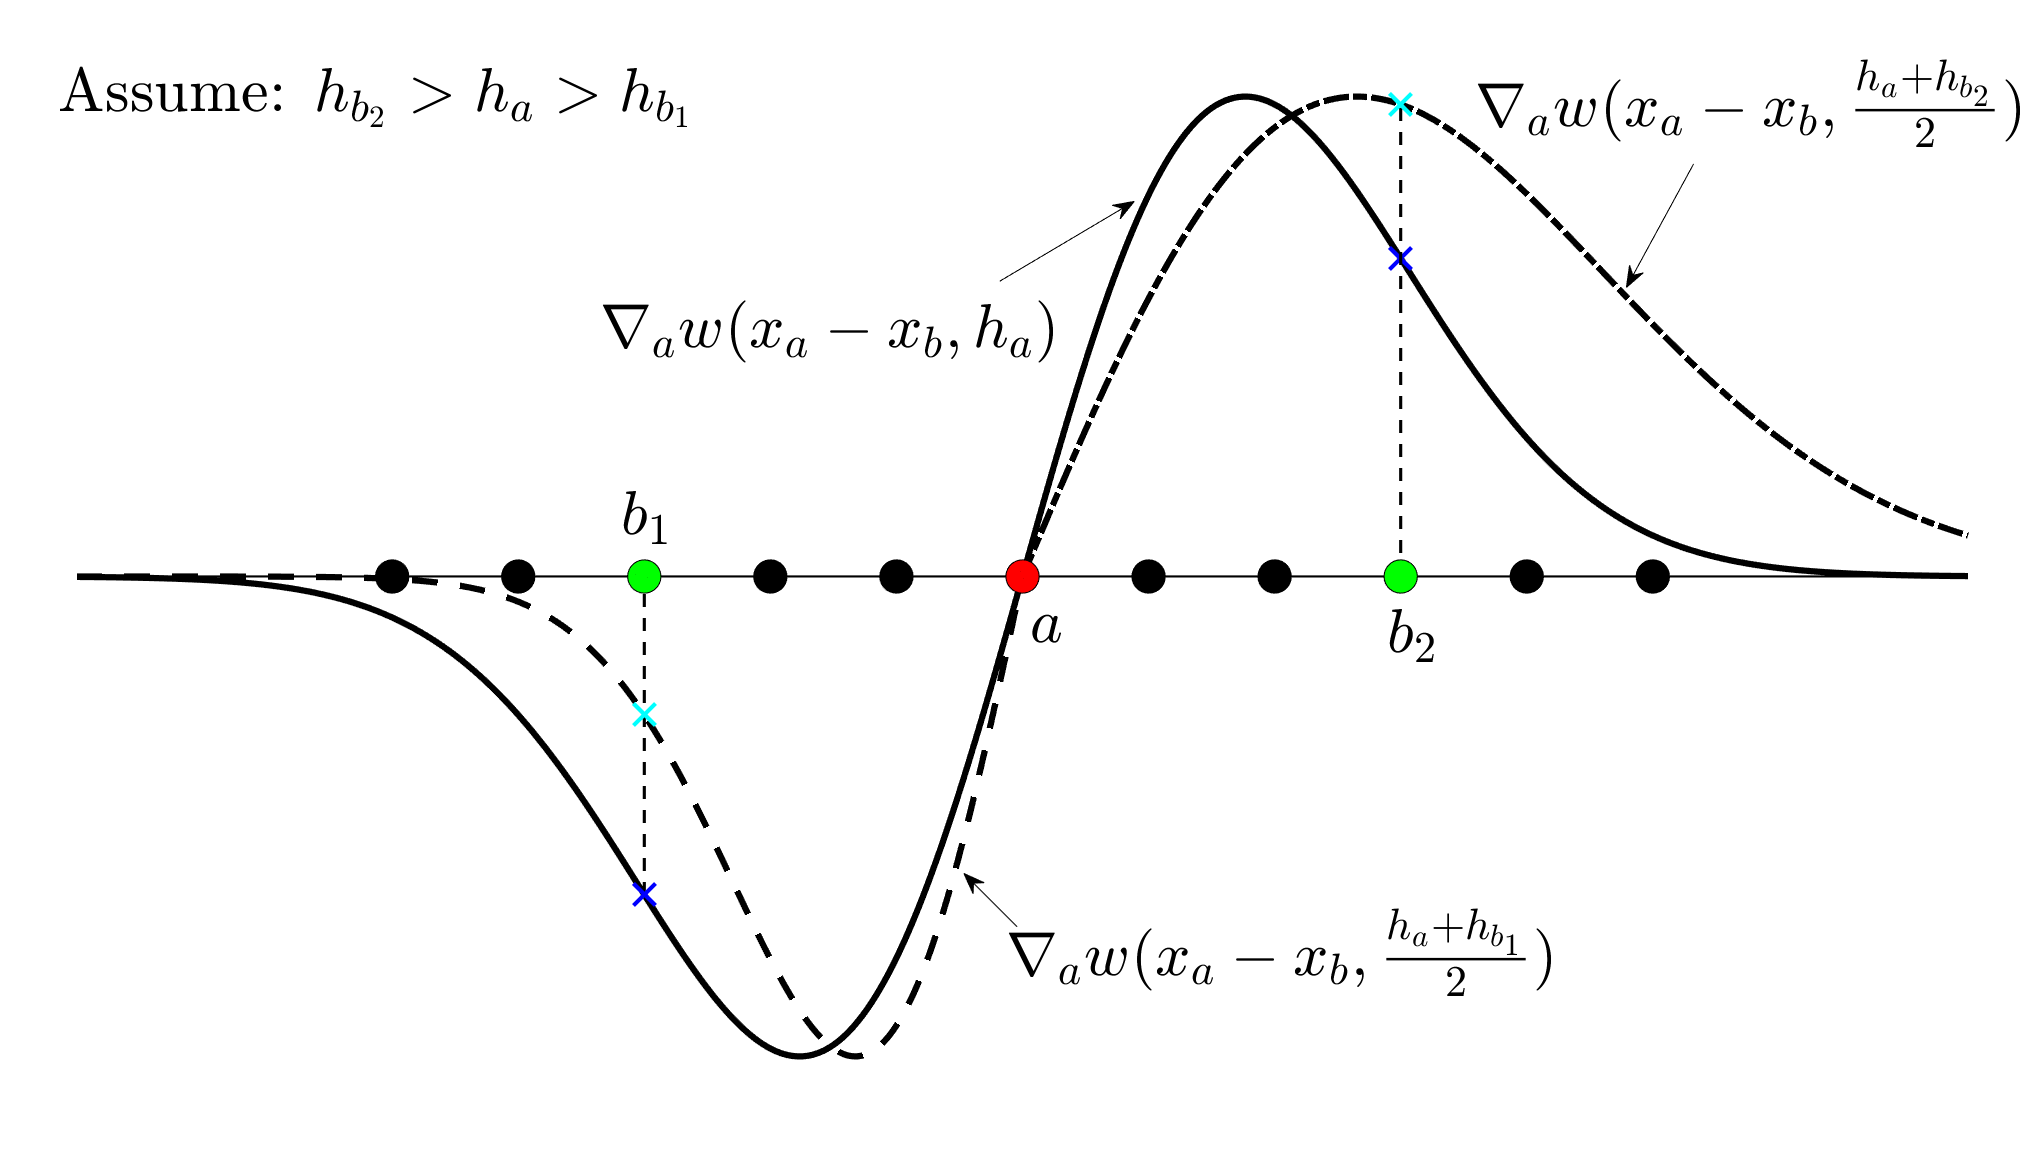
\includegraphics[width=0.90 \textwidth ]{App-Figure/dw-ha}
\caption{In this example, we consider two pairs of particles $(a, b_1)$ and $(a b_2)$. For simplicity, we assume uniform distance between particles. When take $h=\frac{h_a + h_b}{2}$, the actual shape of gradient of kernel function is the combination of two dash curves. It is not anti-symmetric.
We also assume pressure, density and particle mass of all particles are equal. However, the pressure gradient term at particle $a$ in discretized formulation do not cancel out ( $-\dfrac{p_{b_1}}{\rho_{b_1}^2} \nabla_a w_{a b_1}\left(\frac{h_a+h_{b_1}}{2}\right) < -\dfrac{p_{b_2}}{\rho_{b_2}^2} \nabla_a w_{a b2}\left(\frac{h_a+h_{b_1}}{2}\right)$) when smoothing lengths are not equal ($h_{b1} \neq h_{b2}$). This leads to unphysical non-zero pressure gradient, which is the source of numerical oscillation. When smoothing length is uniform in space or take $h = h_a$, the actual shape of gradient of kernel function is the solid curve, which is anti-symmetric. As a consequence, $-\dfrac{p_{b_1}}{\rho_{b_1}^2} \nabla_a w_{a b_1}\left(h\right) = \dfrac{p_{b_2}}{\rho_{b_2}^2} \nabla_a w_{a b2}\left(h\right)$, the unphysical non-zero pressure gradient vanishes.}    
\label{fig:dw-ha}
\end{figure}  

To illustrate the formation and influence of such numerical oscillation, we intentionally create a situation of non-uniform smoothing length by assigning larger smoothing length to boundary ghost particles on left side in 1D shock tube test. Just like discontinuity of physical quantities (for example, the discontinuity at the middle of shock tube test), discontinuity in numerical resolution, in terms of smoothing length, also induces a wave. A perturbation can be observed clearly in the simulation result, starting near the left boundary and propagating into simulation domain. 

In Fig. \ref{fig:Perturbation-ME0-tp1}, no such perturbation when $h = h_a$, which confirms our analysis in Fig. \ref{fig:dw-ha}. 
It needs to emphasize that such perturbation would be created unintentionally in real implementation. The oscillation can actually be observed in 1D shock tube tests of many other papers, even though they are not as obvious as the one in Fig. \ref{fig:Perturbation-ME2}.

\begin{figure}[H]
\centering
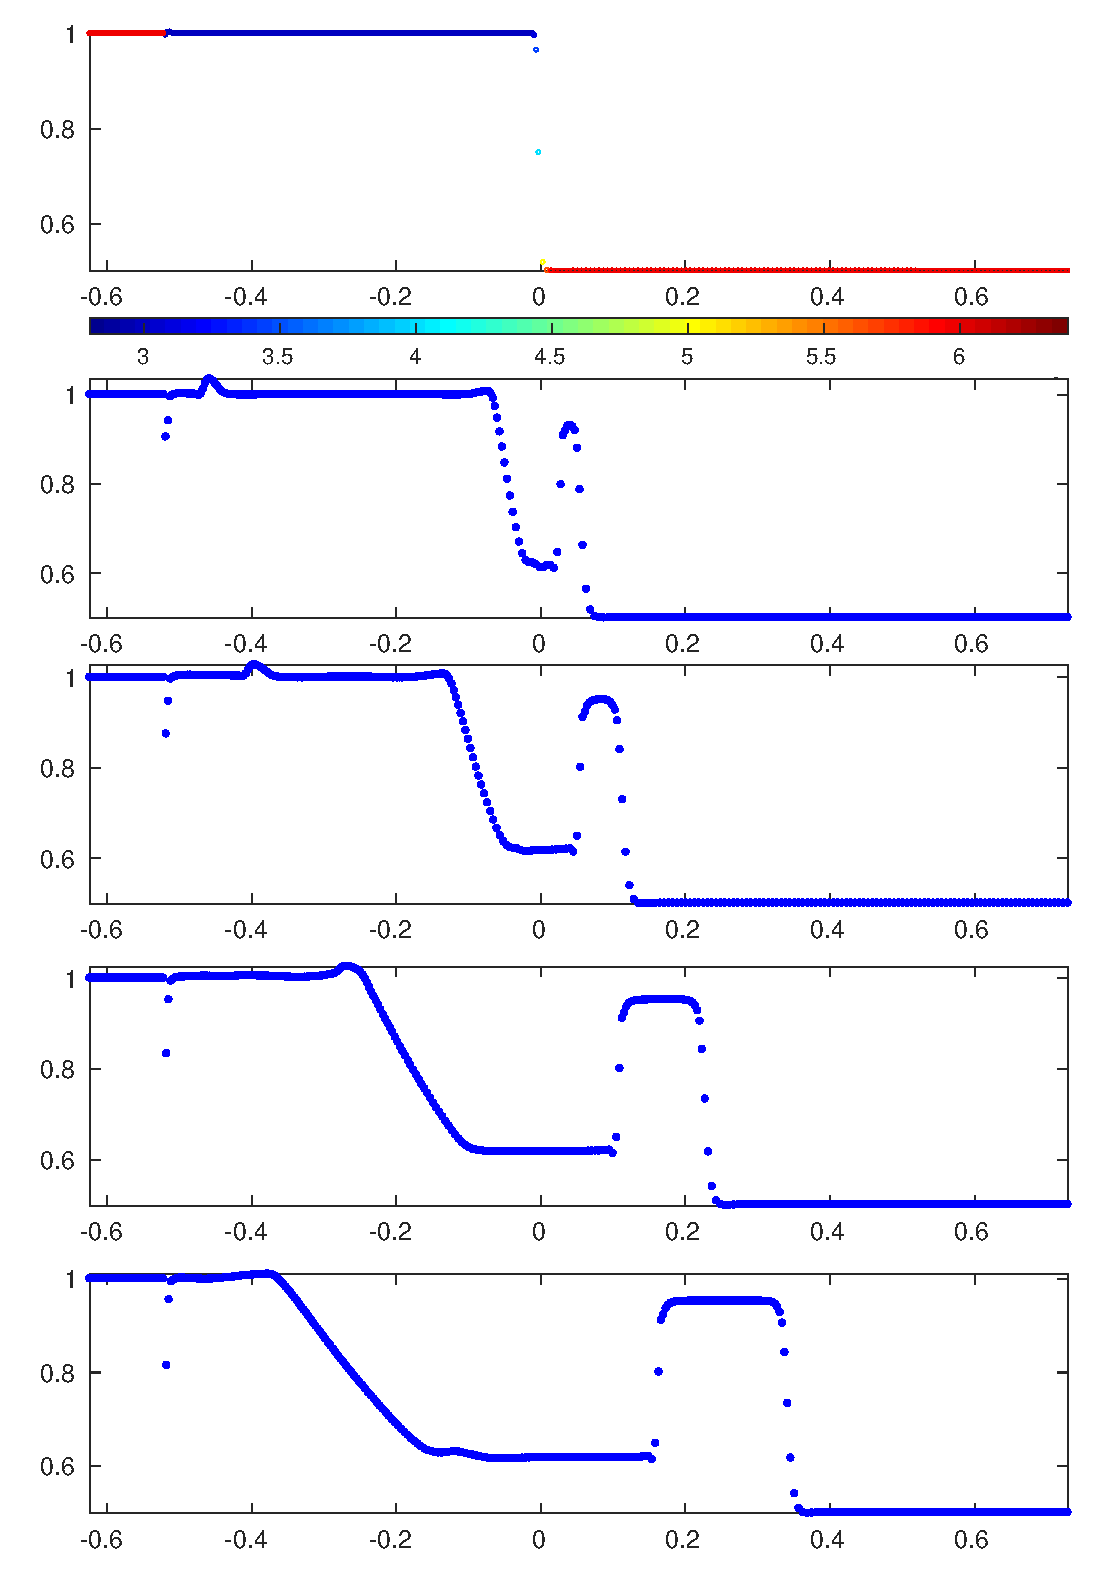
\includegraphics[width=0.90 \textwidth]{App-Figure/Perturbation-ME2}
\caption{Plots of density for 1D shock tube test 2 at different time. In these plots, $x$ axis is location along shock tube, $y$ axis is density. Smoothing length $h = \frac{h_a + h_b}{2}$. The first plot is corresponding to $t=0.001s$, color map is for smoothing length. As shown in first plot, the smoothing length is discontinuous at the left boundary. Such discontinuity induces a numerical perturbation. The second plot to last one are corresponding to $t=0.05s$, $t=0.1s$, $t=0.2s$, $t=0.3s$ respectively. We observe that a numerical perturbation incepts near the left boundary and propogates into the domain. Actually, the smoothing length is also discontinuous at the middle. It should also induce another numerical perturbation. That perturbation has smaller magnitude but stll observable from the figure. It has the same propagating speed as the front of rarefaction. Both perturbations decays in time due to dissipation.}
\label{fig:Perturbation-ME2}
\end{figure}

\begin{figure}[H]
\centering
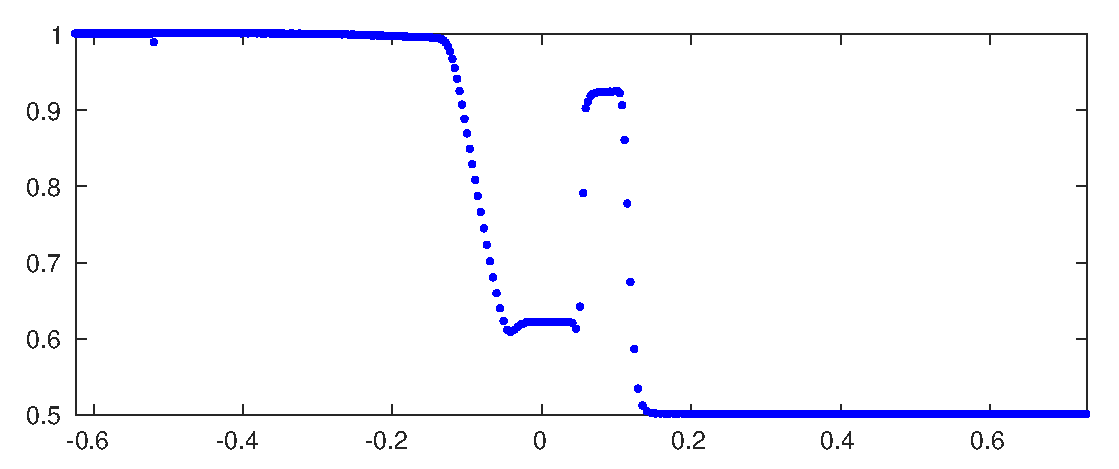
\includegraphics[width=0.90 \textwidth]{App-Figure/Perturbation-ME0-tp1}
\caption{Plots of density for 1D shock tube test 2 at $t=0.1s$. In this test, we still intentionally create non-uniform smoothing length distribution in space by assigning larger smoothing length to wall ghost particles at the left side. But we take $h=h_a$. No numerical perturbation generated near the left boundary.}    
\label{fig:Perturbation-ME0-tp1}
\end{figure}

To summarize, the conditions for generating such numerical oscillation are:
\begin{itemize}
\item Calculate smoothing length by averaging, for example, $h = \frac{h_a + h_b}{2}$.
\textbf{And} 
\item Smoothing length is nonuniform in space.
\end{itemize}
\section*{References}

\bibliography{Reference}

\end{document}
